% part5.tex
\part{复杂图形}

\section{并列的图形}\label{sec:sidebyside}

并列图形所需的命令取决于用户到底想怎样来组织图形。
本节主要讨论三种常见的并列图形方式。
\begin{enumerate}
	\item 多个图像并列于一个图形环境中。
	\item 多个并列的浮动图形,如图~\ref{fig:side:a}~和~\ref{fig:side:b}。
	\item 一图形环境中各个子图的平行排列。
	如子图~\ref{fig:subfig:a}~和~\ref{fig:subfig:b}~并列于图~\ref{fig:subfig}~中。
\end{enumerate}

本节将用下列两种方法构建上述三种并列图形。
\begin{enumerate}
	\item 连续使用 \cmd{includgraphics} 命令。
	\item 并列的小页环境,其中每个都包含一个 \cmd{includegraphics} 命令。
\end{enumerate}
在构造多个并列图形时,很重要的一点是要理解第~\ref{sec:terminology}~节的内容。
并列图形是通过将若干盒子(\cmd{incudegraphics} 或小页)平行放置在一条水平基线上来得到的。

\subsection{单个图形环境中的并列图像}\label{ssec:sidegraphics-singlefig}

对于在单个 \env{figure} 环境中创建并列图像,
尽管使用并列的小页环境能更容易地对齐图像,
不过最简单的办法还是直接连续使用多个 \cmd{includgraphics} 命令。

\subsubsection{使用并列的 includegraphics 命令}

如下代码:
\begin{lstlisting}
\begin{figure} 
	\centering 
	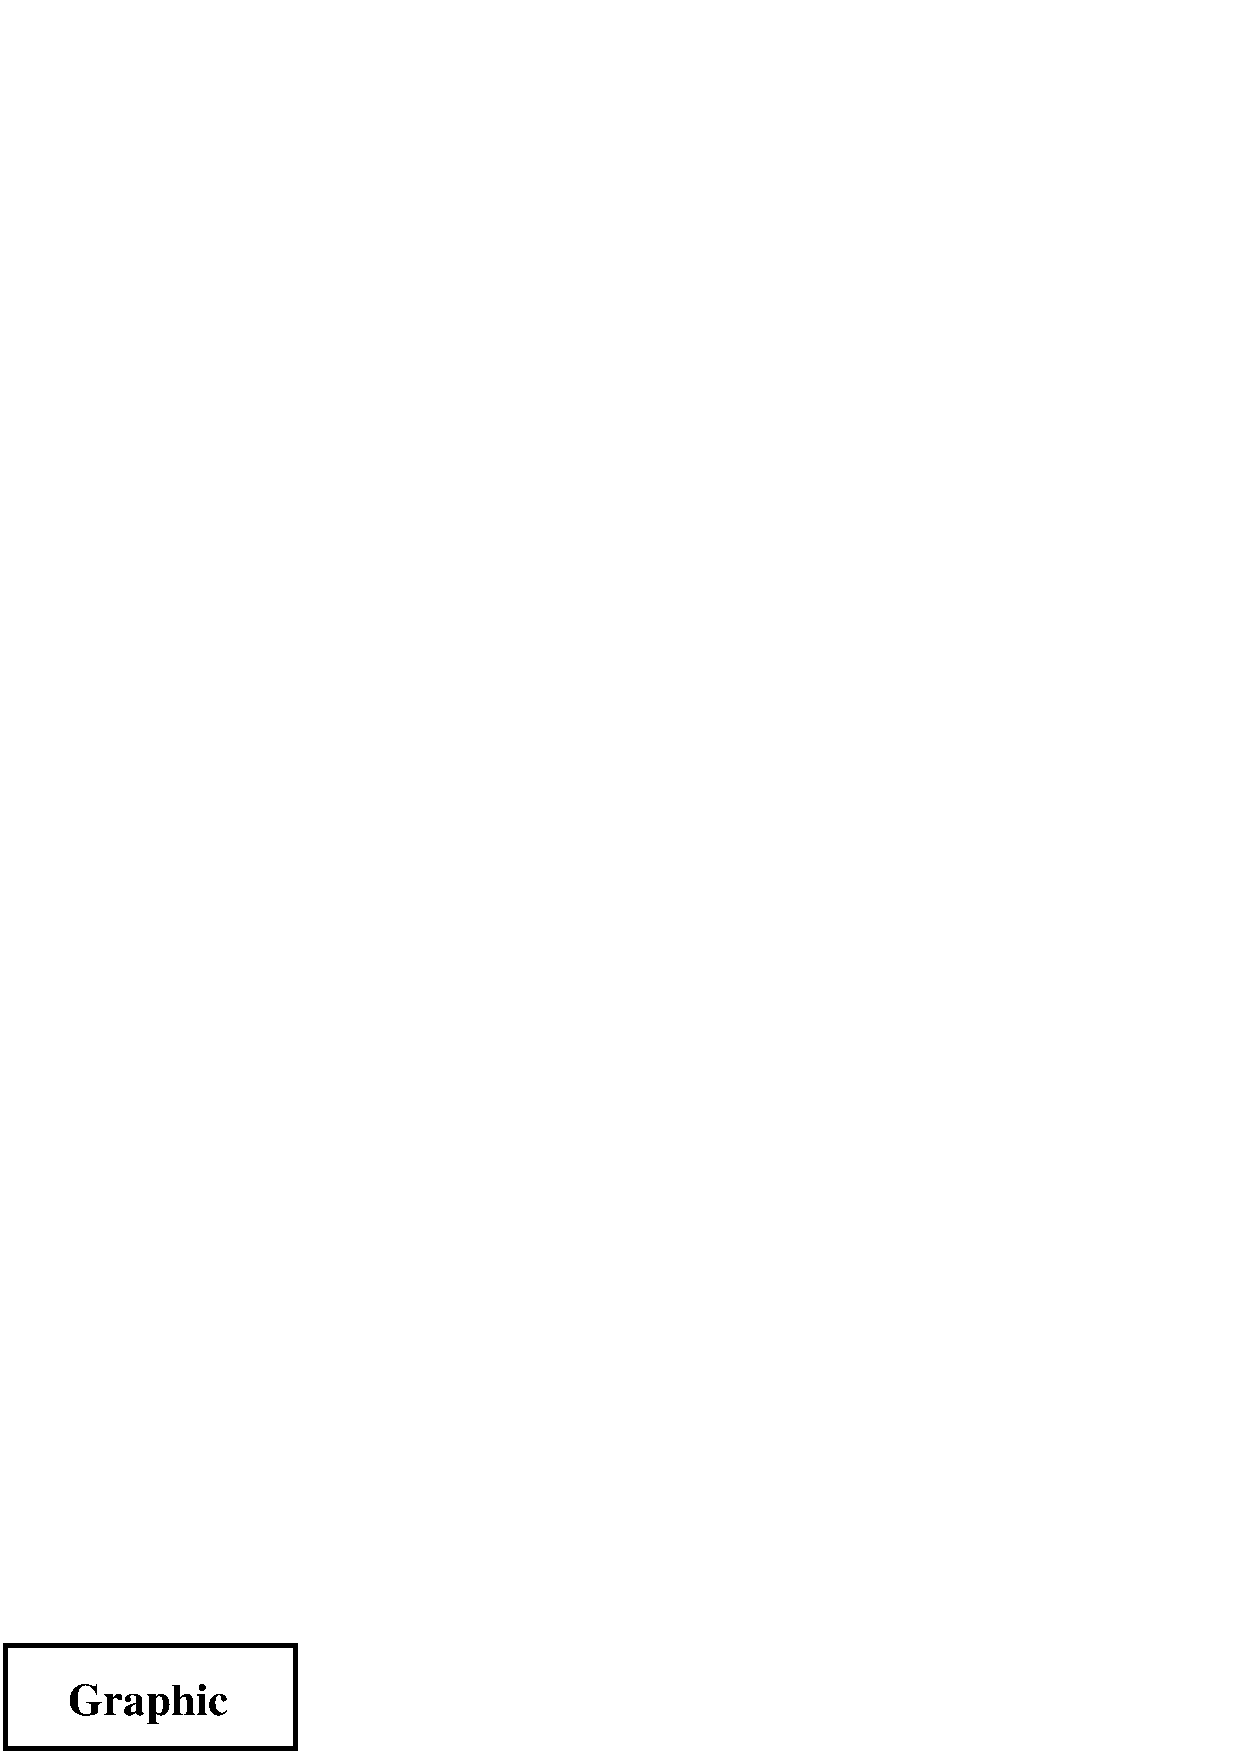
\includegraphics[width=1in]{graphic}% 
	\hspace{1in}% 
	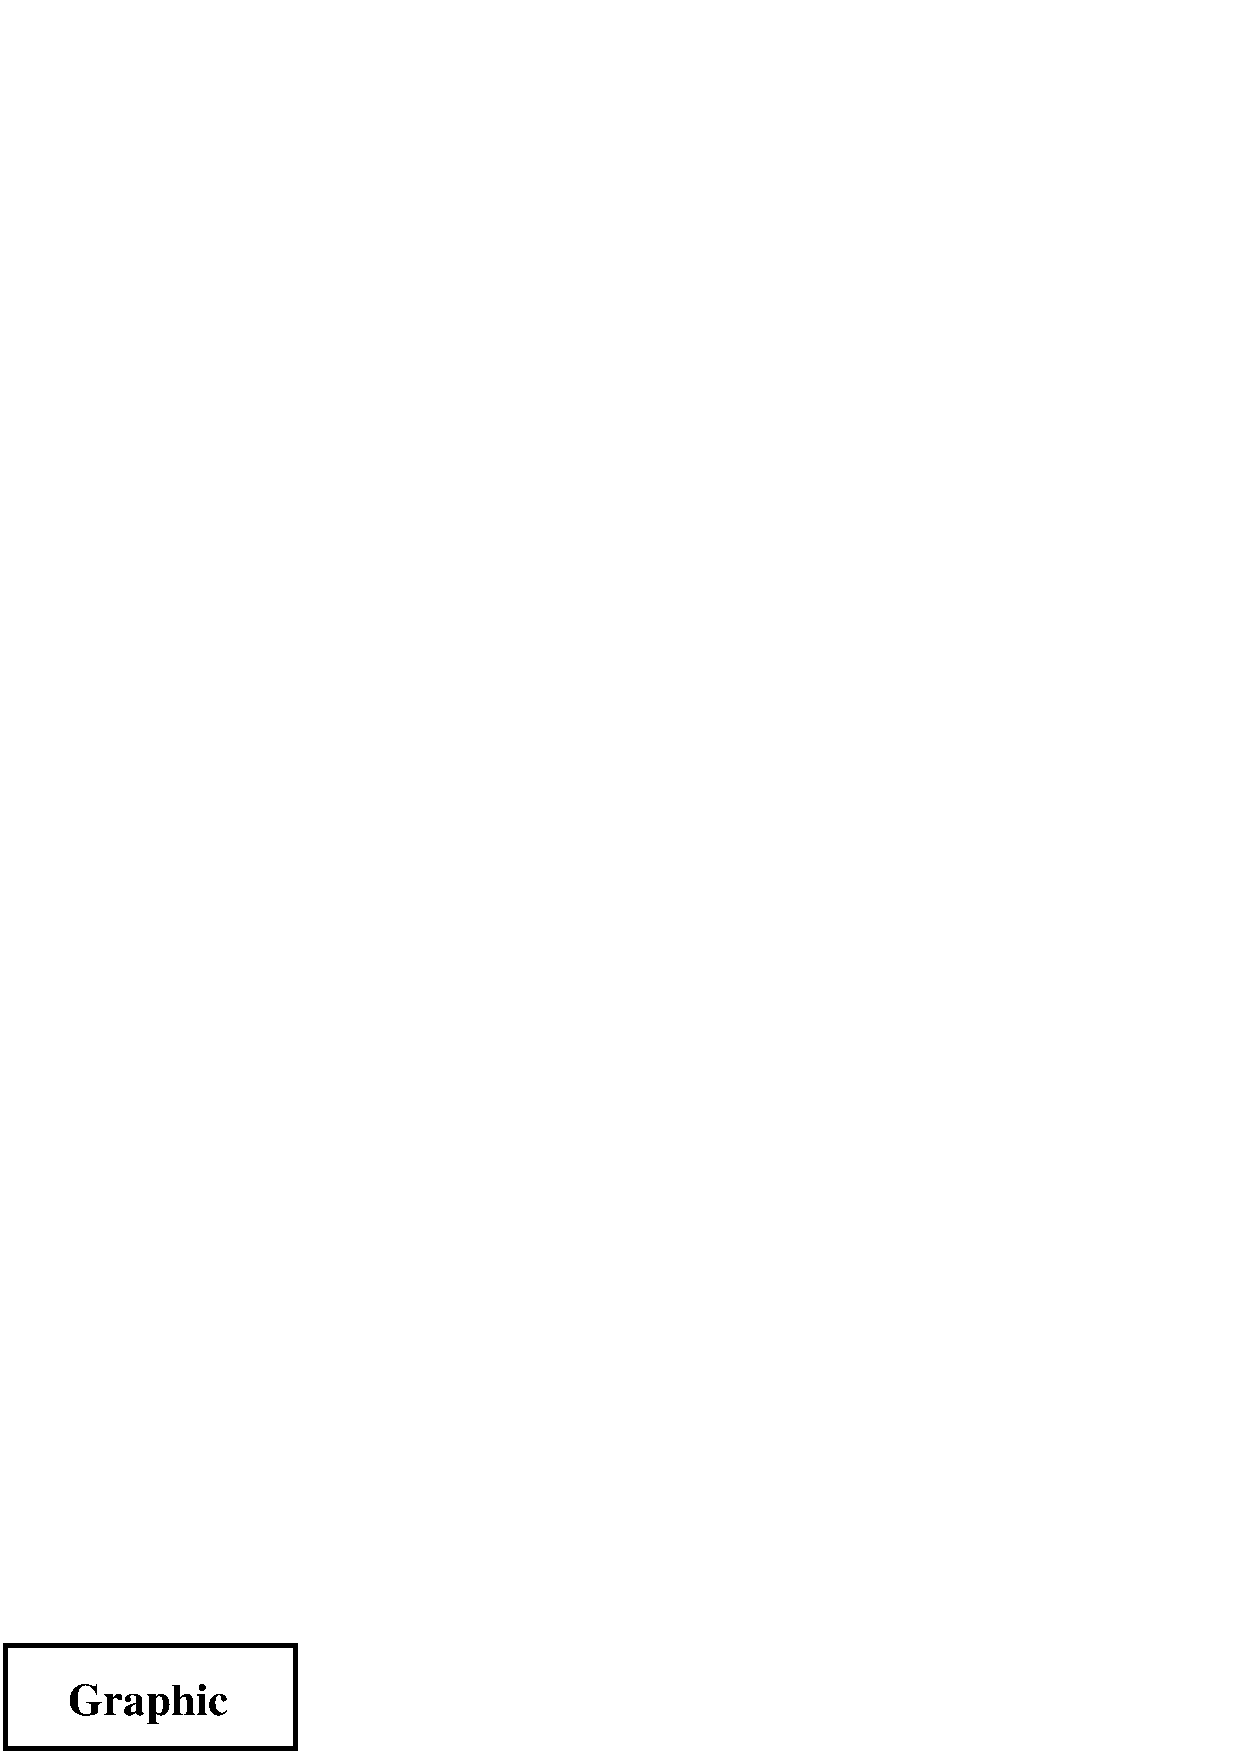
\includegraphics[width=2in]{graphic} 
	\caption{一个 figure 环境中的两幅图像} 
\end{figure}
\end{lstlisting}
会得到如图~\ref{fig:sidegraphics}~的并列图形。
该图形宽度为4英寸(第一幅图1英寸,\cmd{hspace} 间距1英寸,第二幅图2英寸),居中放置。
其中的 \cmd{hspace} 命令可用 \cmd{hfill} 来代替,
这会将图形推向页面的两端边界(见第~\ref{ssec:hspace}~节)。

\begin{figure} 
	\centering 
	\resizebox{1in}{!}{\usebox{\boxgraphic}}% 
	\hspace{1in}% 
	\resizebox{2in}{!}{\usebox{\boxgraphic}}
	\caption{一个 \env{figure} 环境中的两幅图像}\label{fig:sidegraphics}
\end{figure}

\subsubsection{使用并列的小页环境}

将 \cmd{includegraphics} 命令放到小页环境中可以更好地控制图形的对齐方式。例如:
\begin{lstlisting}
\begin{figure} 
	\centering 
	\begin{minipage}[c]{0.5\textwidth} 
		\centering 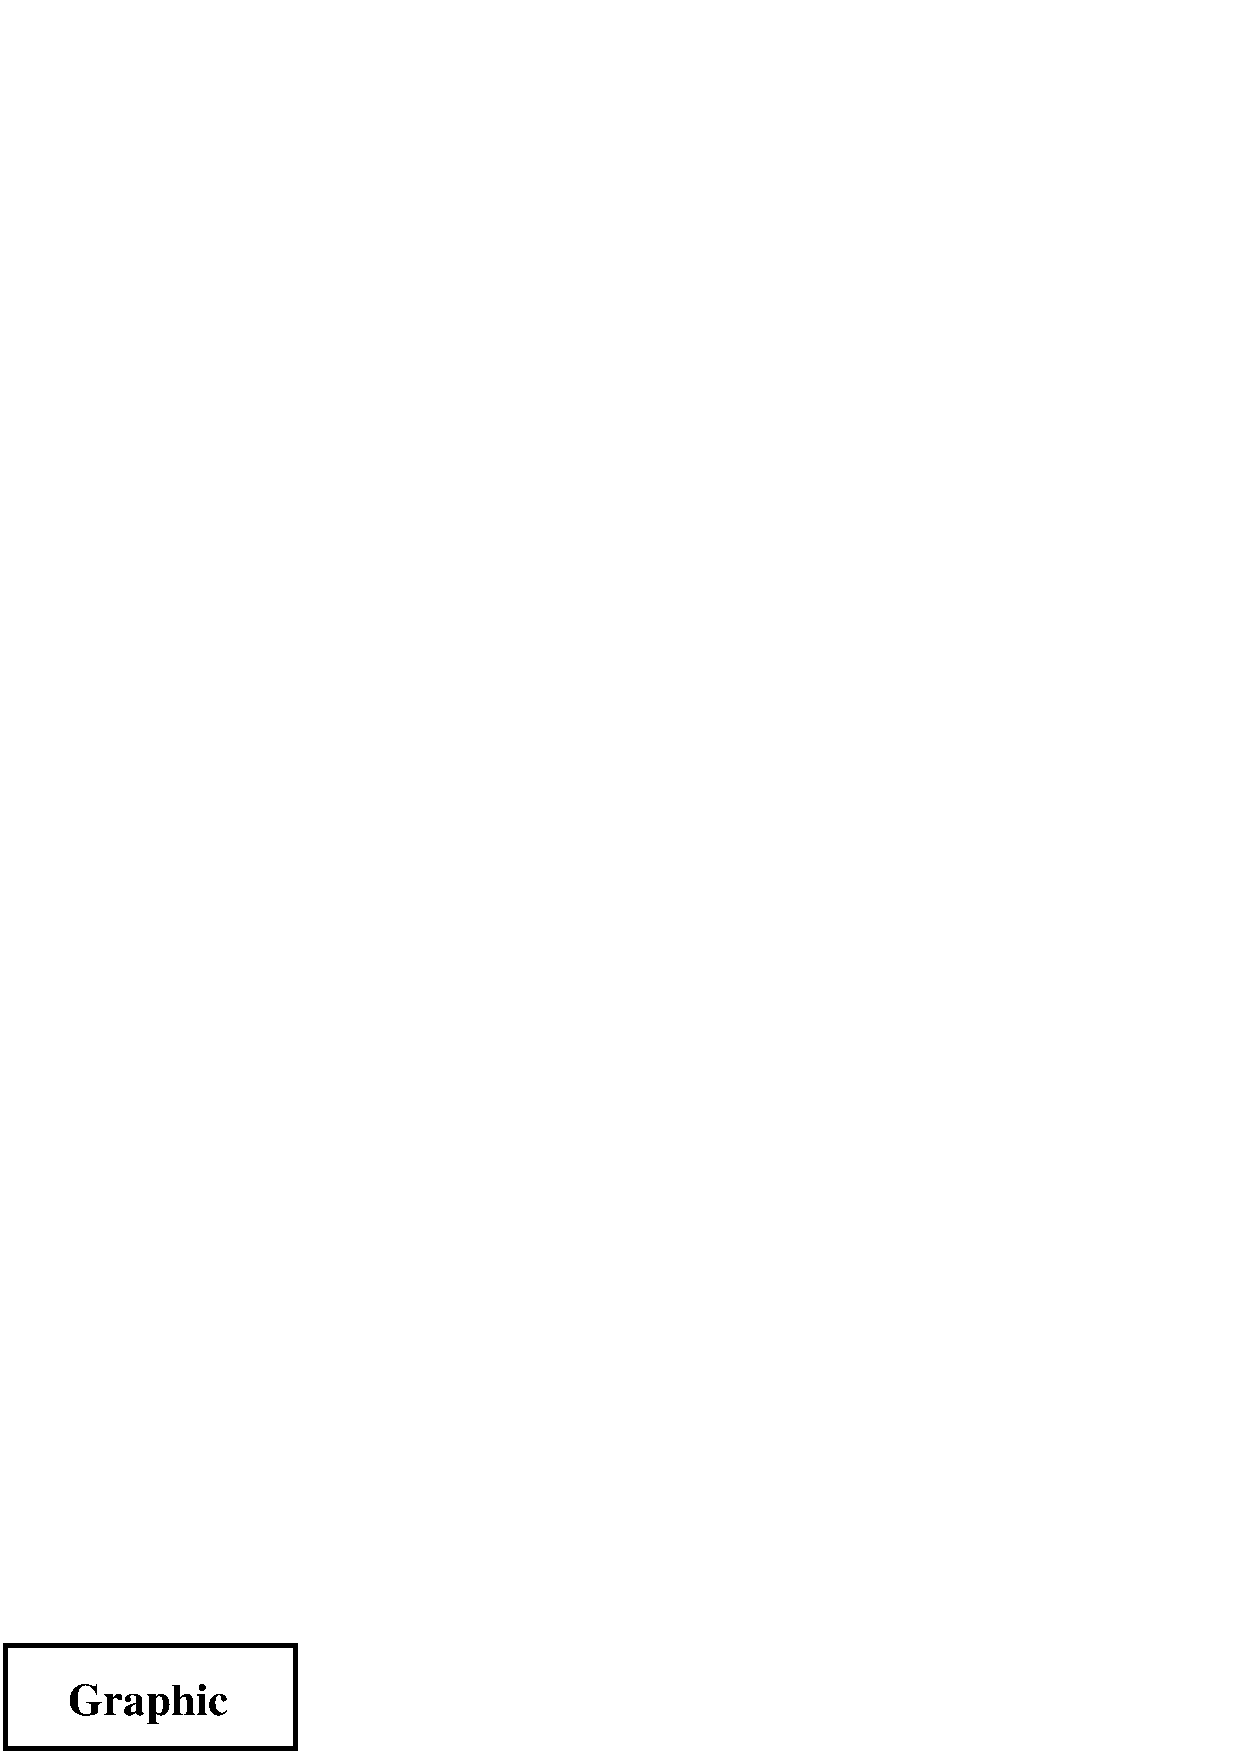
\includegraphics[width=1in]{graphic} 
	\end{minipage}% 
	\begin{minipage}[c]{0.5\textwidth} 
		\centering 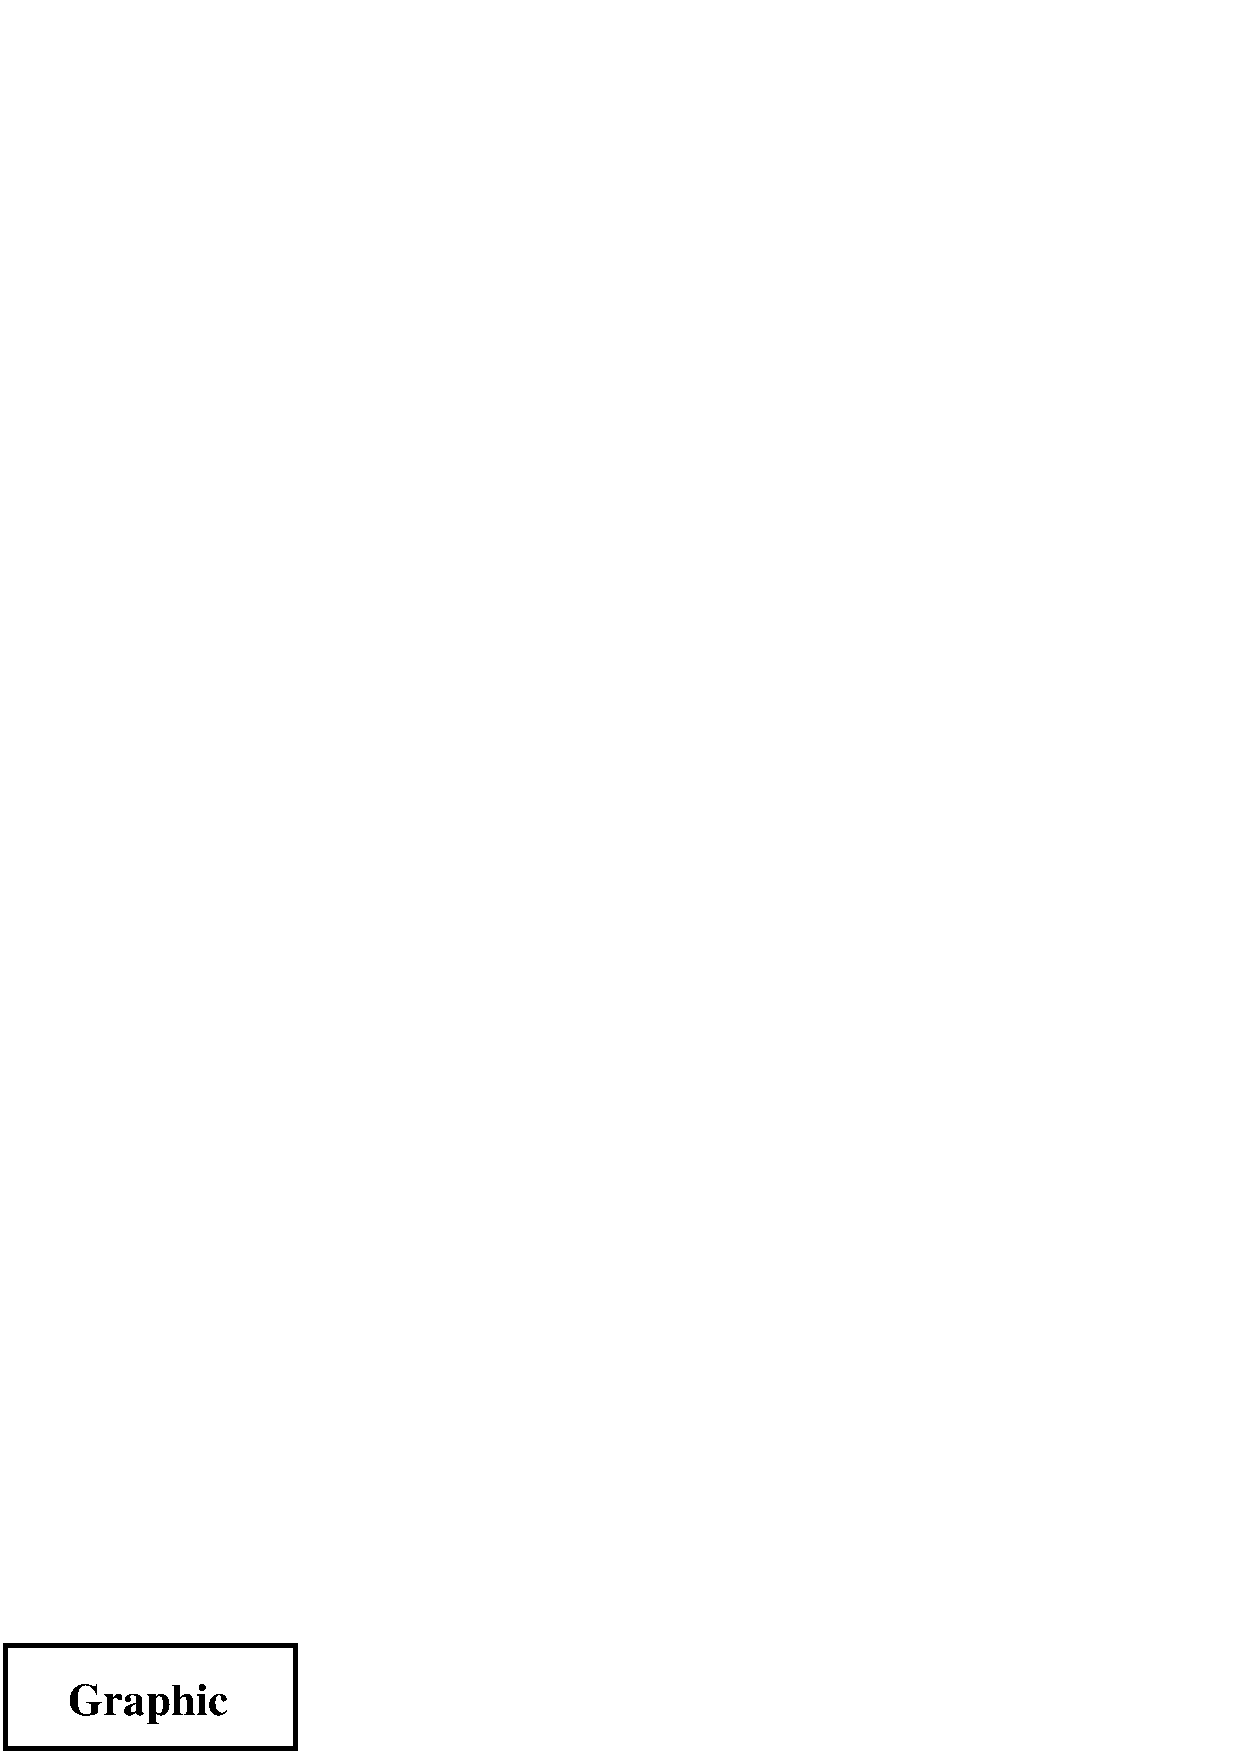
\includegraphics[width=2in]{graphic} 
	\end{minipage} 
	\caption{中间对齐的图像} 
\end{figure}
\end{lstlisting}
生成图~\ref{fig:minipagegraphics}~,其中的图形是中间对齐的。

\begin{figure} 
	\centering 
	\begin{minipage}[c]{0.5\textwidth} 
		\centering
		\resizebox{1in}{!}{\usebox{\boxgraphic}} 
	\end{minipage}% 
	\begin{minipage}[c]{0.5\textwidth} 
		\centering
		\resizebox{2in}{!}{\usebox{\boxgraphic}} 
	\end{minipage} 
	\caption{中间对齐的图像} \label{fig:minipagegraphics}
\end{figure}

对于这个例子,需要注意以下几点:
\begin{itemize}
	\item 如同其它的 \LaTeX{} 对象一样,小页在放置时,它的参考点和当前基线对齐。
	缺省情况下小页使用 \opt{[c]} 选项,将参考点置于其竖直方向的中点。
	选项 \opt{[t]} 将参考点置于小页顶行的基线上,
	而选项 \opt{[b]} 将参考点置于小页底行的基线上(参见第~\ref{ssec:minivalign}~节)。
	
	\item 在第一个 \cmdM{end}{minipage} 后面的 \texttt{\%} 防止在两个小页之间多一个空格
	(参见第~\ref{ssec:hspace} 节)。
	
	\item 当几个并列小页的宽度之和没有达到 $1.0\,\text{\cmd{textwidth}}$ 时,
	可用 \cmd{hspace} 或 \cmd{hfill} 来确定水平间距,详见第~\ref{ssec:hspace}~节。
\end{itemize}


\subsection{并列的浮动图形}\label{ssec:sidefigure}

在上一节中,在一个图形环境中使用多个小页环境可以得到一个由多幅图像组成的浮动图形。
若将  \cmd{caption} 命令放到每个小页环境中,则每个小页环境本身就变成浮动图形。例如:
\begin{lstlisting}
\begin{figure}
	\centering
	%%----start of first figure----
	\begin{minipage}[t]{0.4\linewidth}
		\centering
		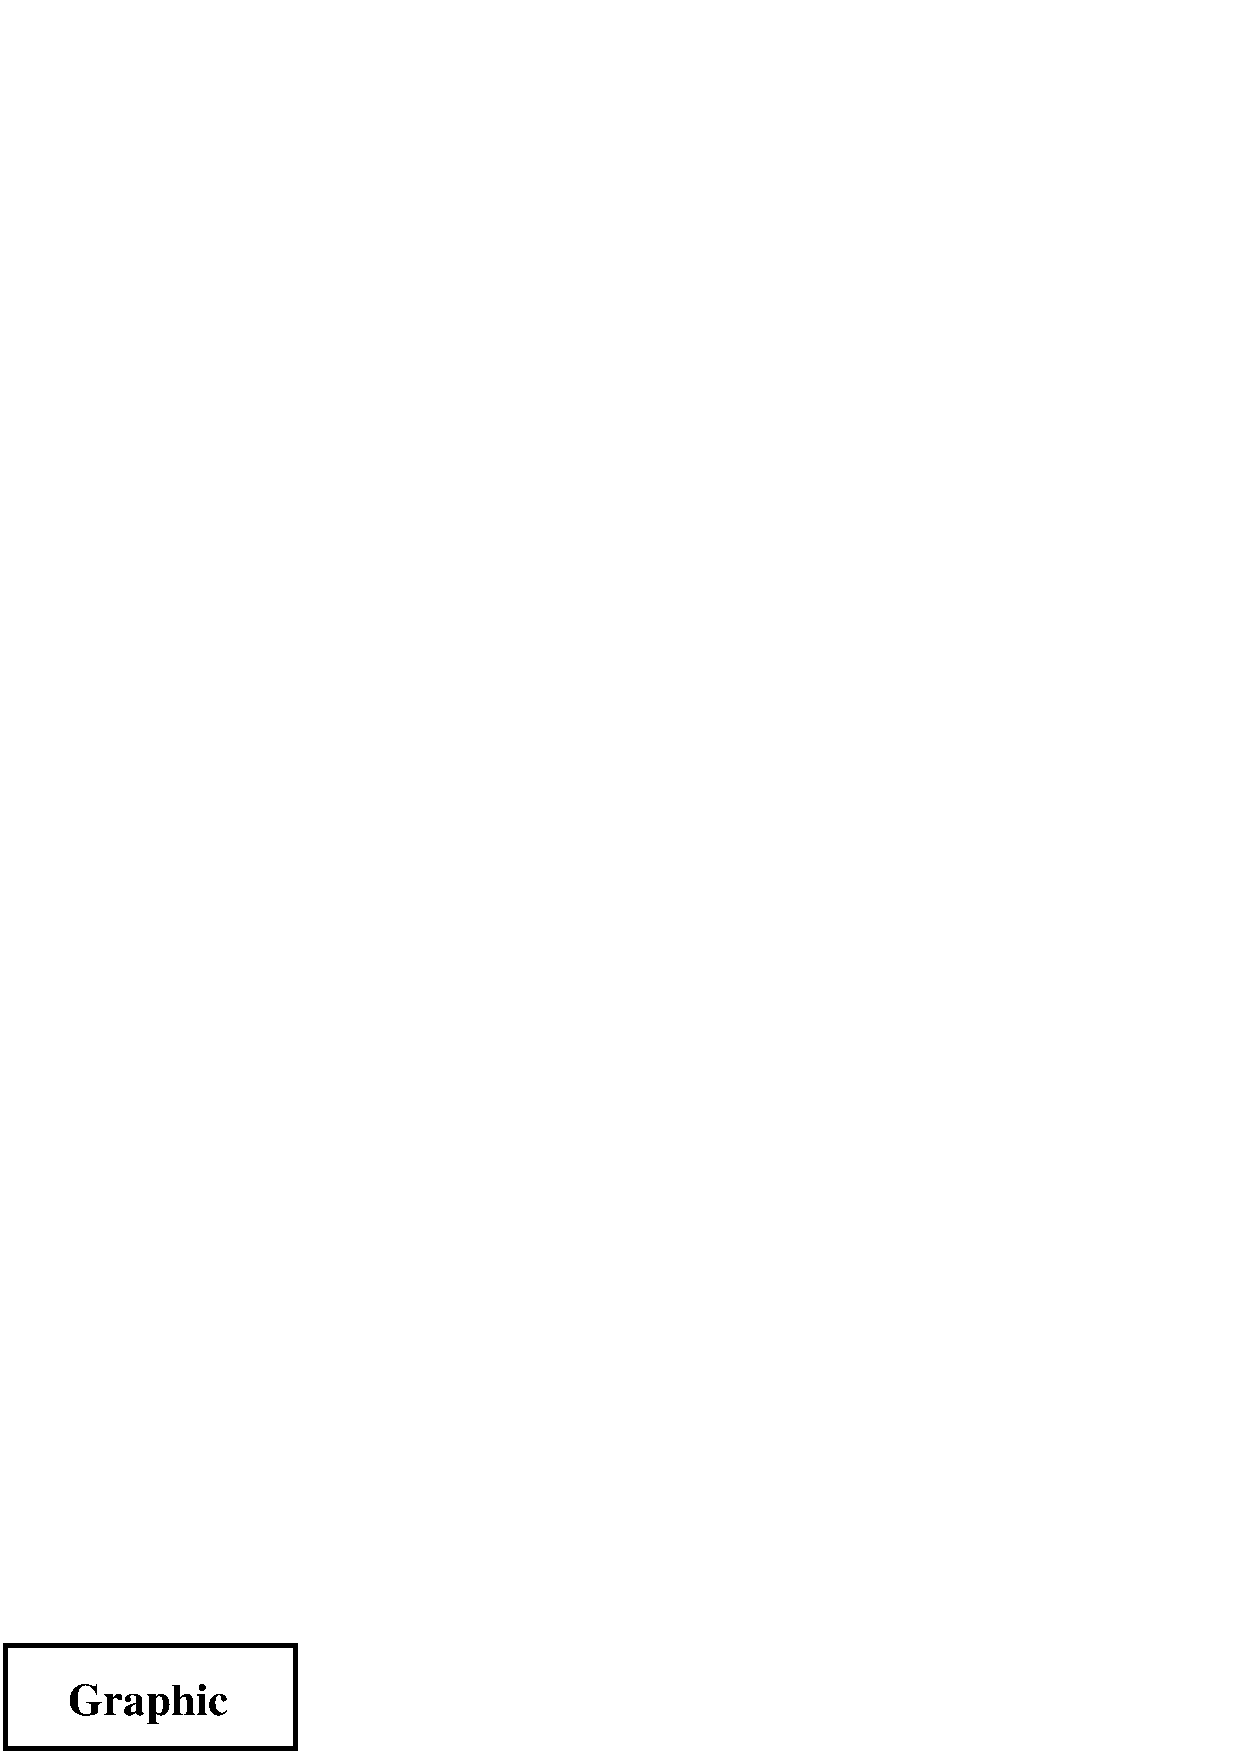
\includegraphics[width=1in]{graphic}
		\caption{Small Box} \label{fig:side:a}
	\end{minipage}%
	\hspace{1cm}%
	%%----start of second figure----
	\begin{minipage}[t]{0.4\linewidth}
		\centering
		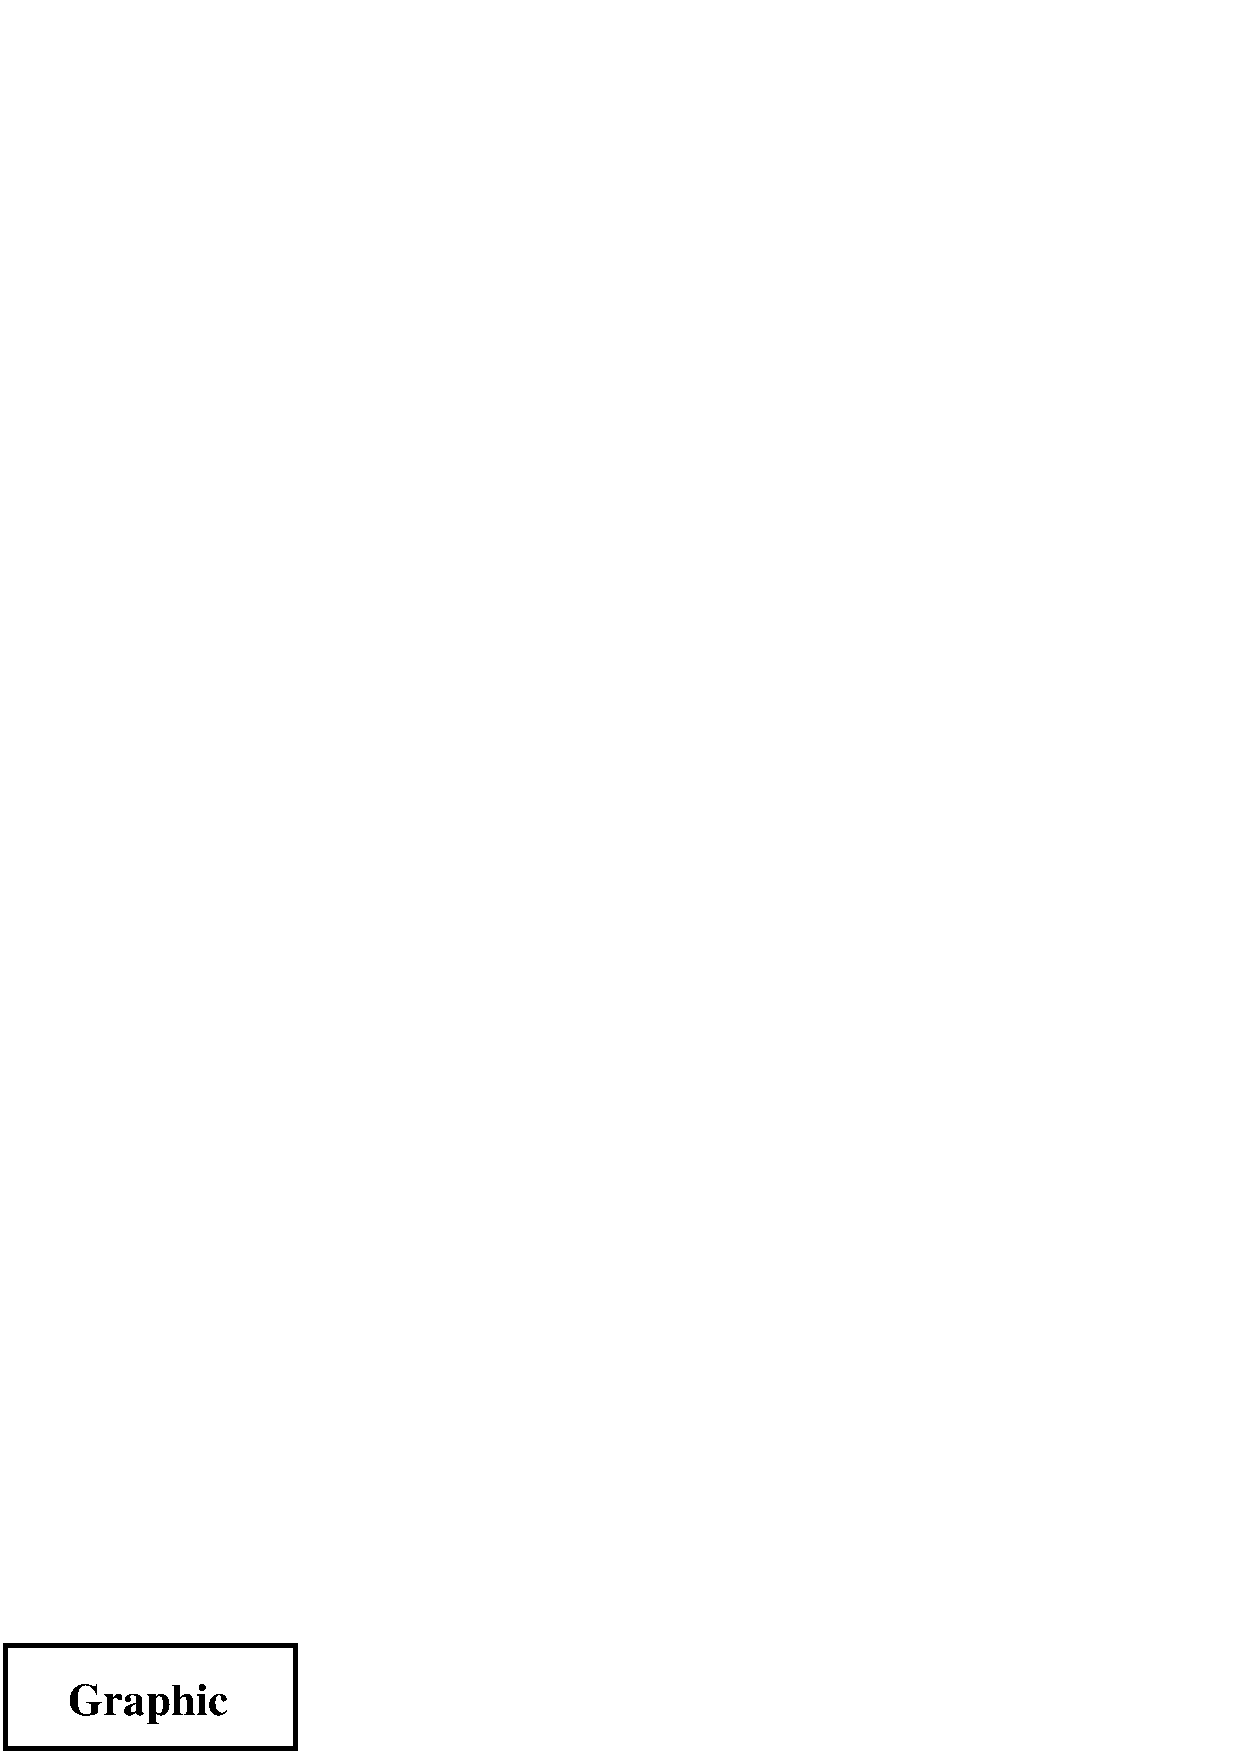
\includegraphics[width=1.5in]{graphic}
		\caption{Big Box} \label{fig:side:b}
	\end{minipage}
\end{figure}
\end{lstlisting}
生成图~\ref{fig:side:a}~和~\ref{fig:side:b}。

\begin{figure}
	\centering
	%%----start of first figure----
	\begin{minipage}[t]{0.4\linewidth}
		\centering
		\resizebox{1in}{!}{\usebox{\boxgraphic}}
		\caption{Small Box} \label{fig:side:a}
	\end{minipage}%
	\hspace{1cm}%
	%%----start of second figure----
	\begin{minipage}[t]{0.4\linewidth}
		\centering
		\resizebox{1.5in}{!}{\usebox{\boxgraphic}}
		\caption{Big Box} \label{fig:side:b}
	\end{minipage}
\end{figure}

关于该例子有几个注记:
\begin{itemize}
	\item 尽管上面的命令只使用了\emph{一}个 \env{figure} 环境,
	但由于每个小页中都包含 \cmd{caption} 命令,所以仍然得到\emph{两}个浮动图形。
	
	\item 两个放置图像的小页环境宽度为 \env{figure} 环境宽度的 $40\,\percent$,
	之间有1厘米的水平间距。
	(注意,在 \cmdM{end}{minipage} 和 \cmdM{hspace}{1cm} 之后的注释会阻止额外的空格,
	从而确保了间距正好是1厘米。)
	默认情况下,图形标题的宽度就是小页环境的宽度。
	使用1厘米的水平间距是为了确保标题之间有空白(无论对长标题还是很宽的图像)。
	此外,标题的宽度也可以用 \pkg{caption} 宏包的 \opt{margin} 或 \opt{width} 关键字进行控制
	(参见表~\ref{tab:caption-formatopt})。
	
	\item 紧接着 \cmdM{begin}{figure} 的 \cmd{centering} 命令使得两个小页环境以及之间的空白在 \env{figure} 环境中居中放置。
		
	\item 小页内部的 \cmd{centering} 命令使得图像在小页环境内部居中放置。
\end{itemize}

\subsection{并列的子图形}\label{ssec:sidesubfigure}

在某些情况下,有时会希望将并列的图形组成一组,同时其中的每一幅图都保持其独立性。
\pkgi{subcaption} 宏包的 \cmdi{subcaptionbox} 命令(详见第~\ref{sec:subcaption-pkg} 节)
可以将一组独立的图像作为一个 \env{figure} 环境中的子图。
例如:
\begin{lstlisting}
\usepackage{subcaption}
...
\begin{figure}
	\centering
	%%----start of first subfigure----
	\subcaptionbox{Small Box with a Long Caption%
		\label{fig:subfig:a} %% label for first subfigure
		}{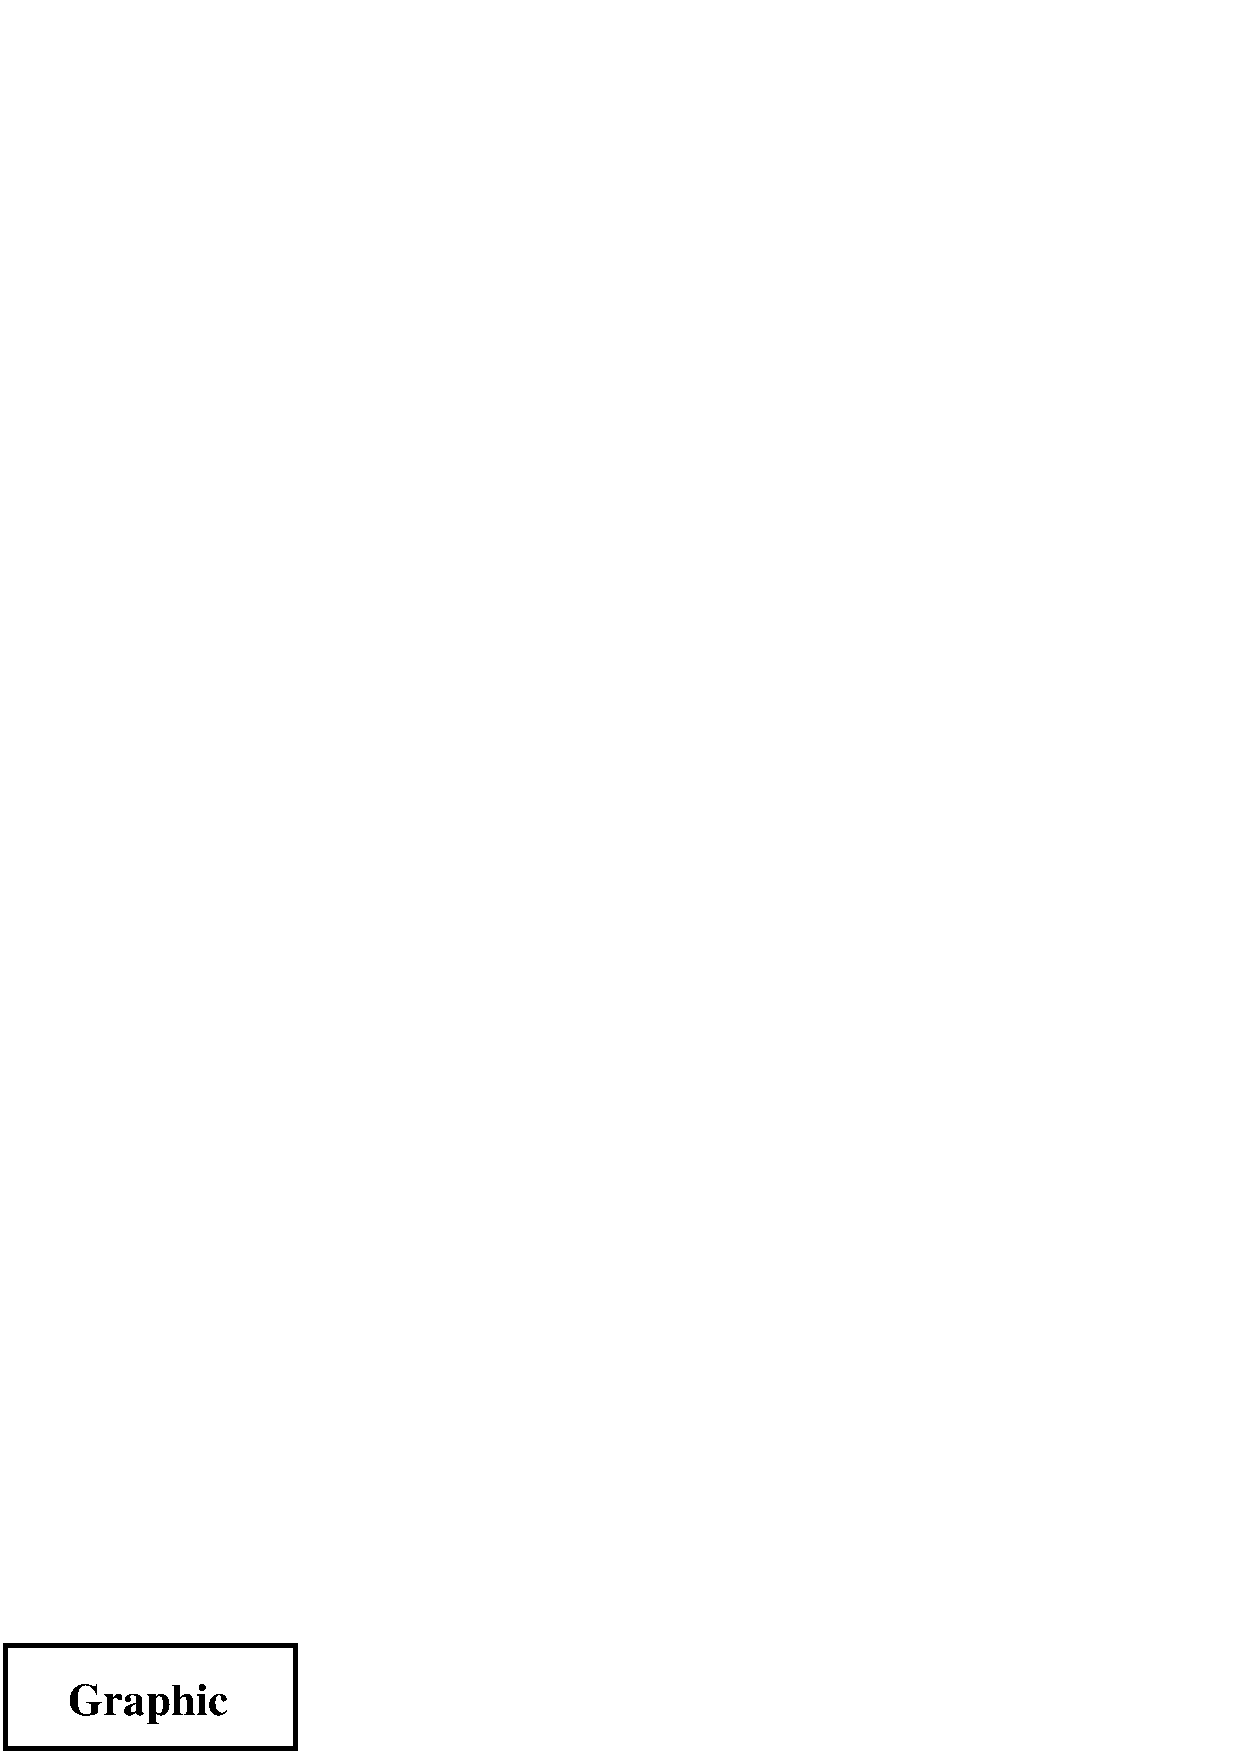
\includegraphics[width=1.1in]{graphic}}
	\hspace{1in}
	%%----start of second subfigure----
	\subcaptionbox{Big Box%
		\label{fig:subfig:b} %% label for second subfigure
		}{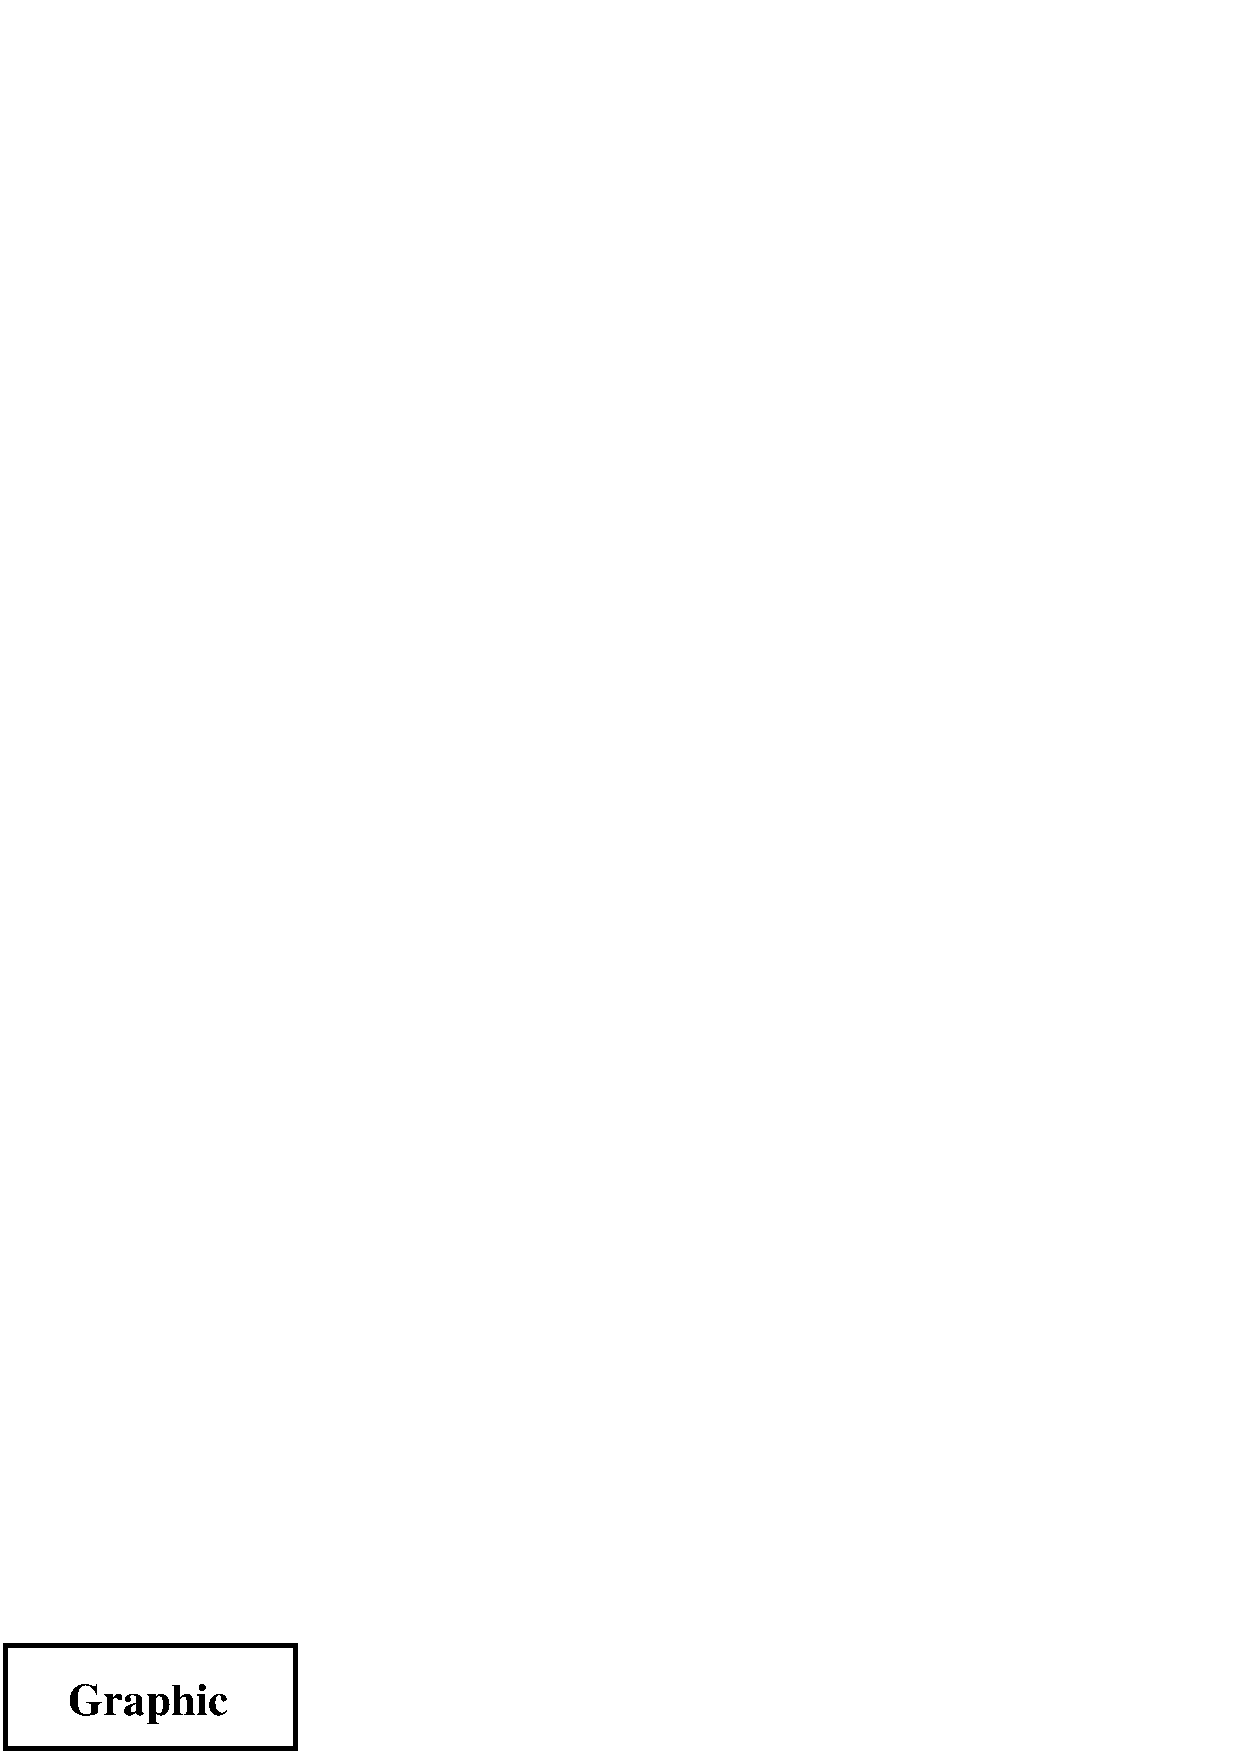
\includegraphics[width=1.5in]{graphic}}
	\caption{Two Subfigures}
	\label{fig:subfig} %% label for entire figure
\end{figure}
\end{lstlisting}
生成图~\ref{fig:subfig}。
表~\ref{tab:ref-subfig} 展示了用于如何引用图~\ref{fig:subfig} 中子图的命令。
其中带 \texttt{*} 的命令 \cmd{ref*} 和 \cmd{subref*} 需要导入 \pkg{hyperref} 宏包,
效果是生成没有超链接的引用。

\begin{figure}
	\centering
	%%----start of first subfigure----
	\subcaptionbox{Small Box with a Long Caption%
		\label{fig:subfig:a} %% label for first subfigure
	}{\resizebox{1.1in}{!}{\usebox{\boxgraphic}}}
	\hspace{1in}
	%%----start of second subfigure----
	\subcaptionbox{Big Box%
		\label{fig:subfig:b} %% label for second subfigure
	}{\resizebox{1.5in}{!}{\usebox{\boxgraphic}}}
	\caption{Two Subfigures}
	\label{fig:subfig} %% label for entire figure
\end{figure}


\begin{table}
	\centering
	\caption{图~\ref{fig:subfig} 的子图引用命令及其结果}\label{tab:ref-subfig}
	\begin{tabular}{lc}
		\toprule
		引用命令 & 输出 \\
		\midrule
		\cmdM{subref}{fig:subfig:a} & \subref{fig:subfig:a} \\
		\cmdM{subref*}{fig:subfig:a} & \subref*{fig:subfig:a} \\
		\cmdM{ref}{fig:subfig:a} & \ref{fig:subfig:a} \\
		\cmdM{ref*}{fig:subfig:a} & \ref*{fig:subfig:a} \\
		\cmdM{subref}{fig:subfig:b} & \subref{fig:subfig:b} \\
		\cmdM{subref*}{fig:subfig:b} & \subref*{fig:subfig:b} \\
		\cmdM{ref}{fig:subfig:b} & \ref{fig:subfig:b} \\
		\cmdM{ref*}{fig:subfig:b} & \ref*{fig:subfig:b} \\
		\cmdM{ref}{fig:subfig} & \ref{fig:subfig} \\
		\cmdM{ref*}{fig:subfig} & \ref*{fig:subfig} \\
		\bottomrule
	\end{tabular}
\end{table}

\subsubsection{并列子图的宽度}

使用 \cmd{subcaptionbox} 创建的子图宽度默认为插入内容的自然宽度。
由于子图~\ref{fig:subfig:a} 只包含 \cmd{includegraphics} 插图命令,
因此其标题宽度取决于图片的宽度。
\cmd{subcaptionbox} 命令还提供了一个可选项用于控制子图的宽度,
这样标题就可以和子图宽度一样了。
例如,
\begin{lstlisting}
\begin{figure}
	\centering
	%%----start of first subfigure----
	\subcaptionbox{Small Box with a Long Caption%
		\label{fig:specwid:subfig:a} %% label for first subfigure
	}[0.45\linewidth]{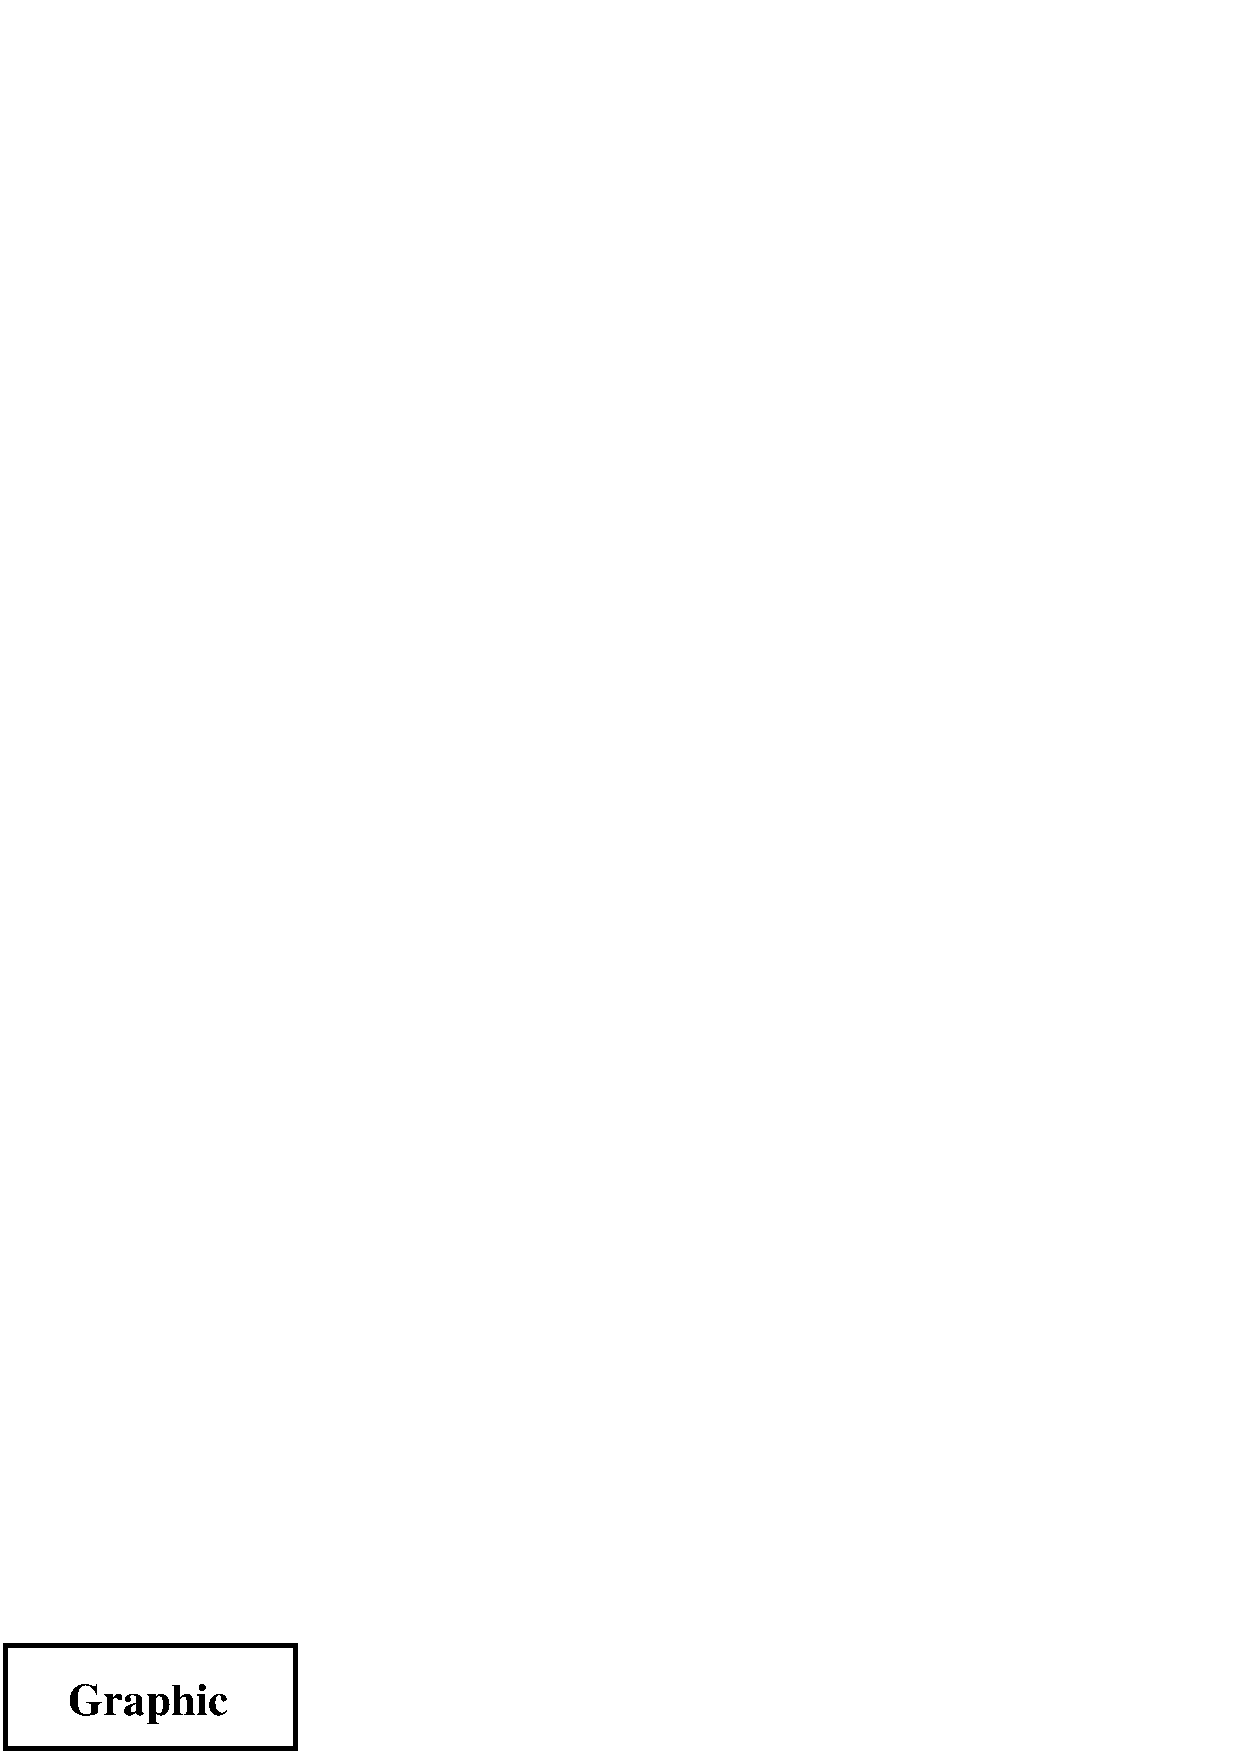
\includegraphics[width=1.1in]{graphic}}
	\hfill
	%%----start of second subfigure----
	\subcaptionbox{Big Box%
		\label{fig:specwid:subfig:b} %% label for second subfigure
	}[0.45\linewidth]{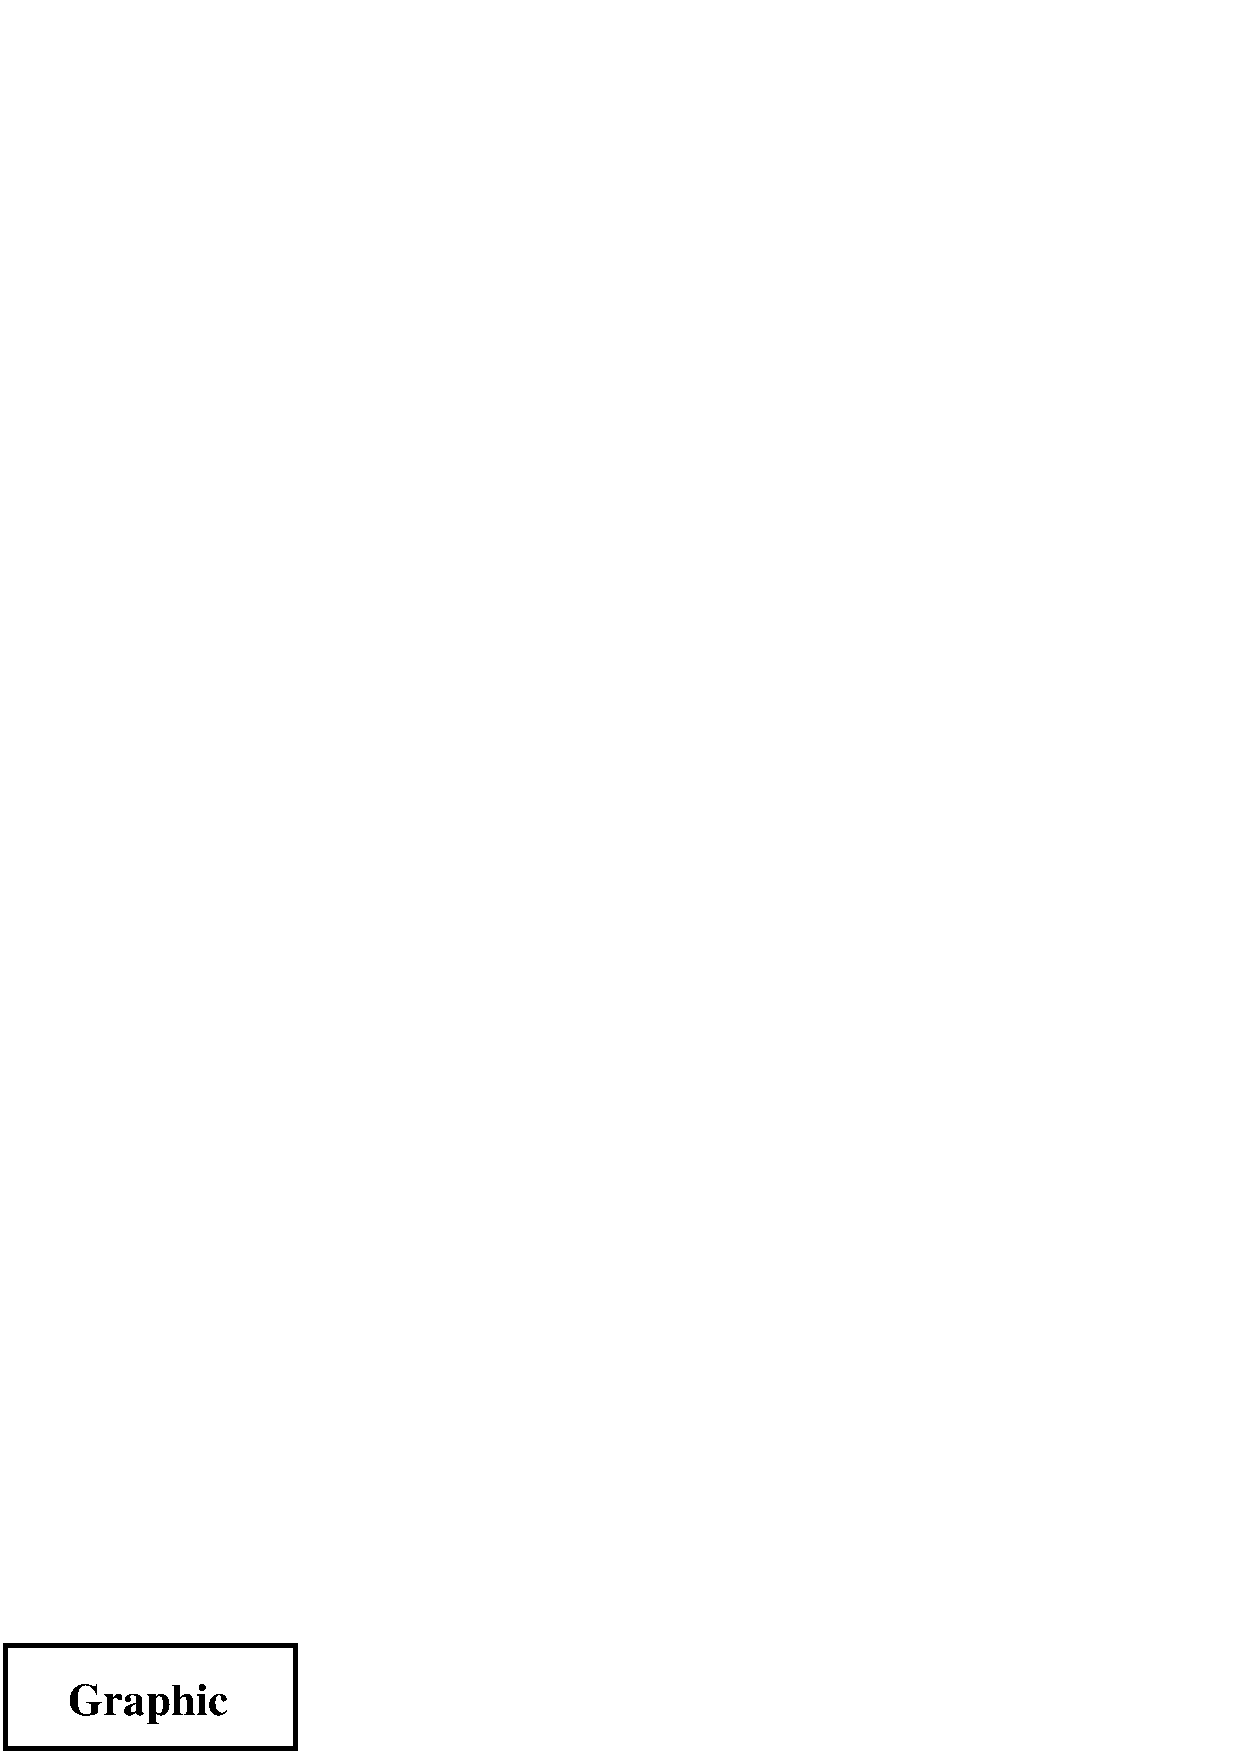
\includegraphics[width=1.5in]{graphic}}
	\caption{Two Subfigures}
	\label{fig:specwid:subfig} %% label for entire figure
\end{figure}
\end{lstlisting}
生成图~\ref{fig:specwid:subfig},
其中包含了子图~\ref{fig:specwid:subfig:a} 和~\ref{fig:specwid:subfig:b}。

\begin{figure}
	\centering
	%%----start of first subfigure----
	\subcaptionbox{Small Box with a Long Caption%
		\label{fig:specwid:subfig:a} %% label for first subfigure
	}[0.45\linewidth]{\resizebox{1.1in}{!}{\usebox{\boxgraphic}}}
	\hfill
	%%----start of second subfigure----
	\subcaptionbox{Big Box%
		\label{fig:specwid:subfig:b} %% label for second subfigure
	}[0.45\linewidth]{\resizebox{1.5in}{!}{\usebox{\boxgraphic}}}
	\caption{Two Subfigures}
	\label{fig:specwid:subfig} %% label for entire figure
\end{figure}

\section{标题中分开的小页环境}

第~\ref{ssec:sidefigure} 节描述了如何通过在小页环境中同时使用插图命令和 \cmd{caption} 命令来构建并列图形。
本节将介绍如何通过在不同的小页环境中使用插图命令和 \cmd{caption} 命令来获得更好的对齐效果。

在图~\ref{fig:side:a}~和~\ref{fig:side:b}中,
并列的小页环境使用了 \opt{[t]}~选项,进而使得两幅图形的基线对齐。
这对于非旋转的图形没有任何问题,而且使得两标题的顶部对齐。
不过,如果图形的底部不对齐的话(如其中一图形被旋转),就会发生问题。例如:
\begin{lstlisting}
\begin{figure}
	\centering
	%%----start of first figure----
	\begin{minipage}[t]{.4\linewidth}
		\centering
		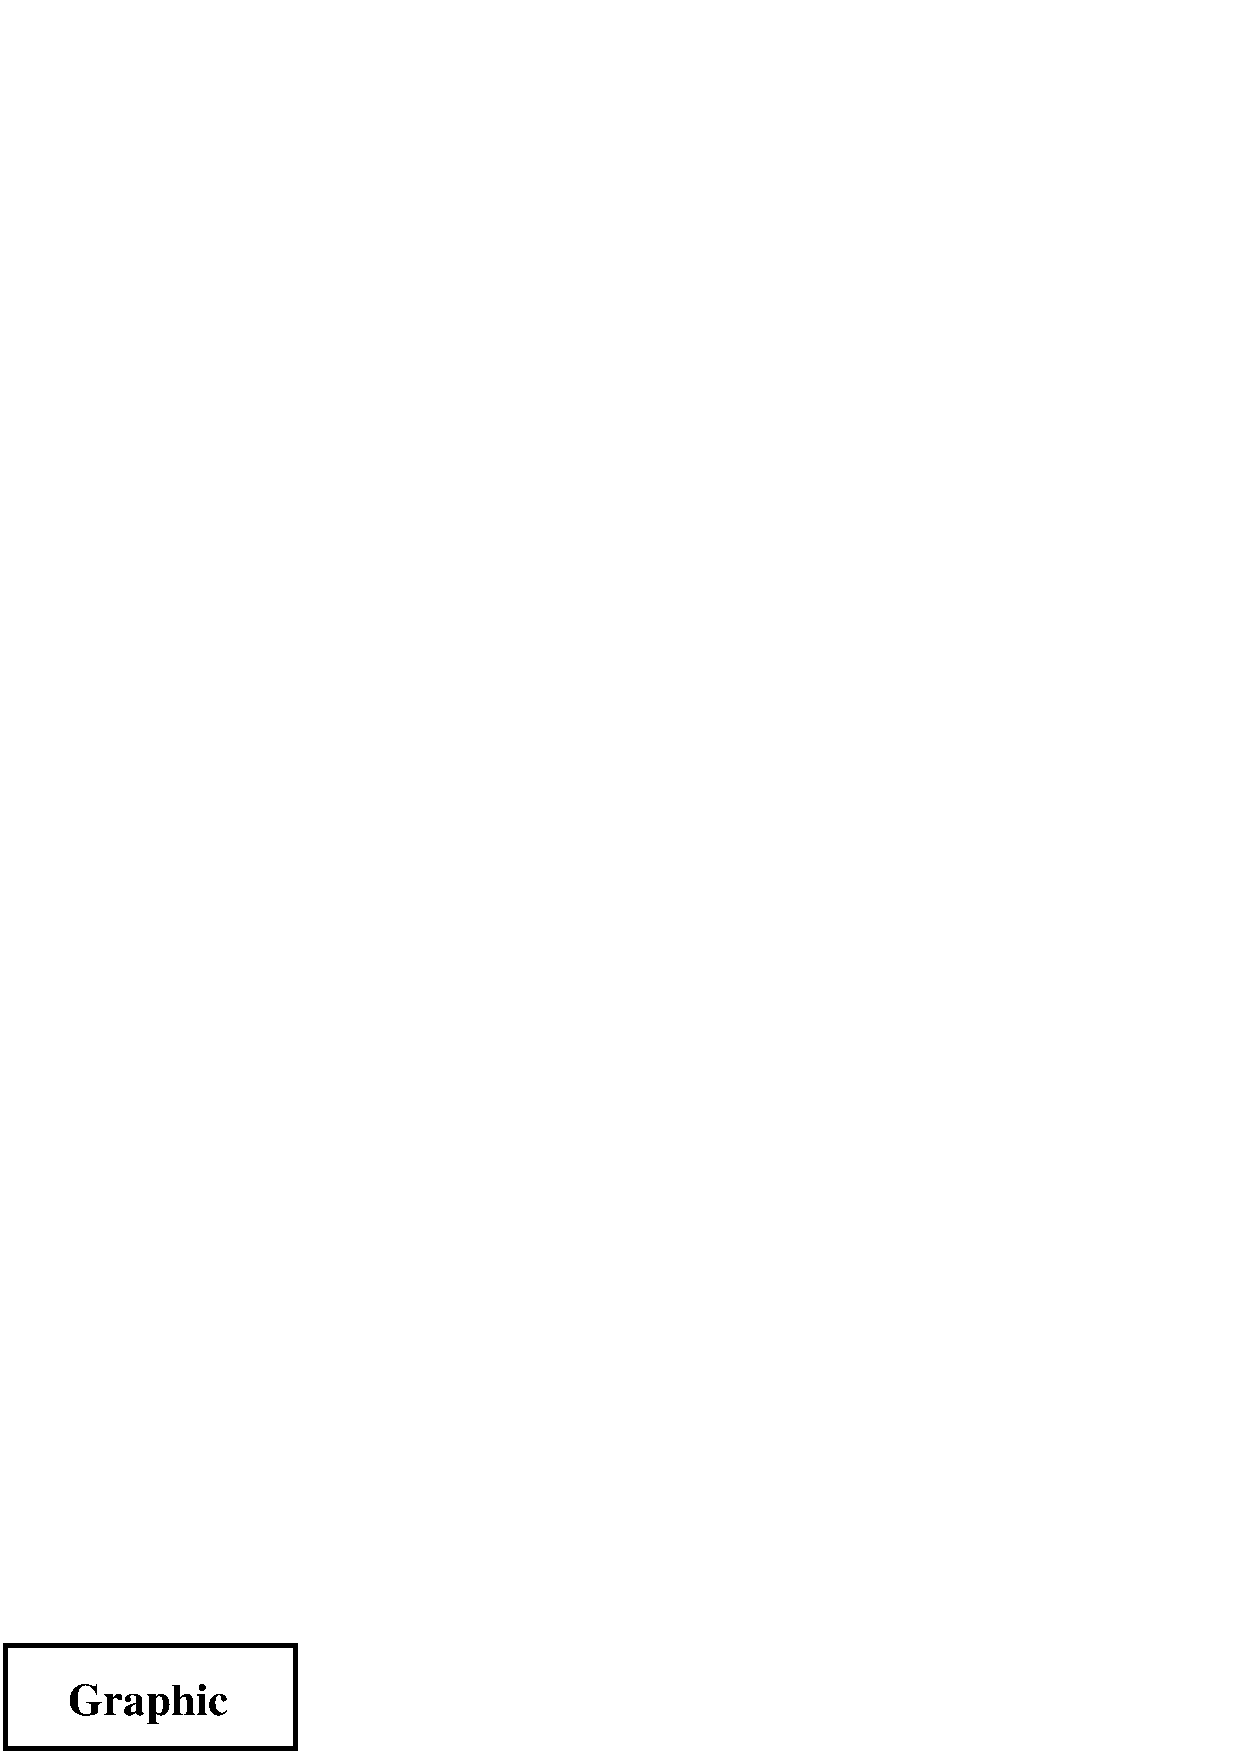
\includegraphics[width=2cm]{graphic}
		\caption{Box with a Long Caption}
	\end{minipage}%
	\hspace{1cm}%
	%%----start of second figure----
	\begin{minipage}[t]{.4\linewidth}
		\centering
		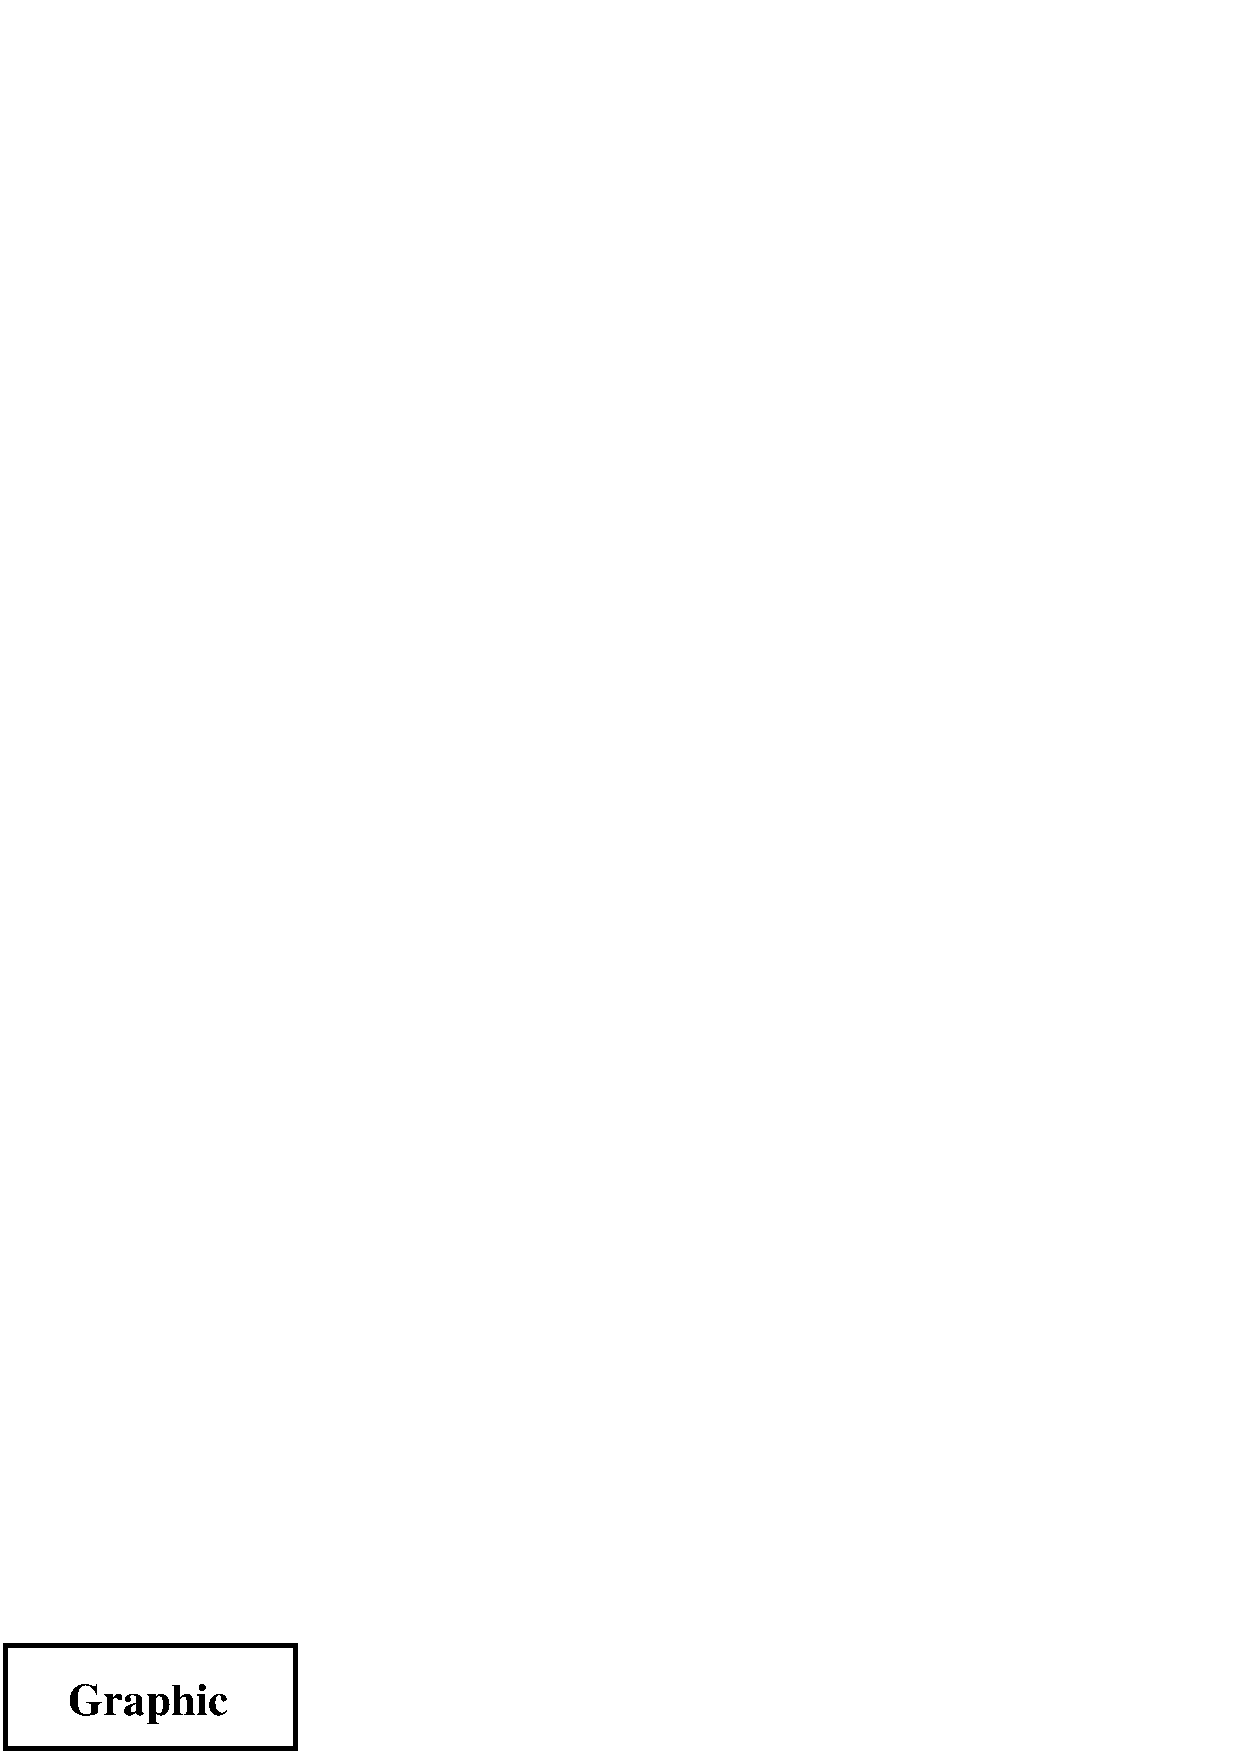
\includegraphics[width=2cm,angle=-30]{graphic}
		\caption{Rotated Box}
	\end{minipage}%
\end{figure}
\end{lstlisting}
生成图~\ref{fig:mininonrot}~和~\ref{fig:minirot},
我们可以看到这里两幅图形的标题并不对齐。
而若只使用小页的 \opt{[b]} 选项,会使得标题的最后一行对齐,并不能解决问题。

\begin{figure}
	\centering
	%%----start of first figure----
	\begin{minipage}[t]{.4\linewidth}
		\centering
		\resizebox{2cm}{!}{\usebox{\boxgraphic}}
		\caption{Box with a Long Caption}\label{fig:mininonrot} 
	\end{minipage}%
	\hspace{1cm}%
	%%----start of second figure----
	\begin{minipage}[t]{.4\linewidth}
		\centering
		\rotatebox{-30}{\resizebox{2cm}{!}{\usebox{\boxgraphic}}}
		\caption{Rotated Box}\label{fig:minirot} 
	\end{minipage}%
\end{figure}

一种解决办法是在创建两行小页环境,并把图形和标题分开放置:
第一行放置图形,第二行放置标题。例如:
\begin{lstlisting}
\begin{figure}
	\centering
	%%----start of first figure graphics----
	\begin{minipage}[b]{.4\linewidth}
		\centering
		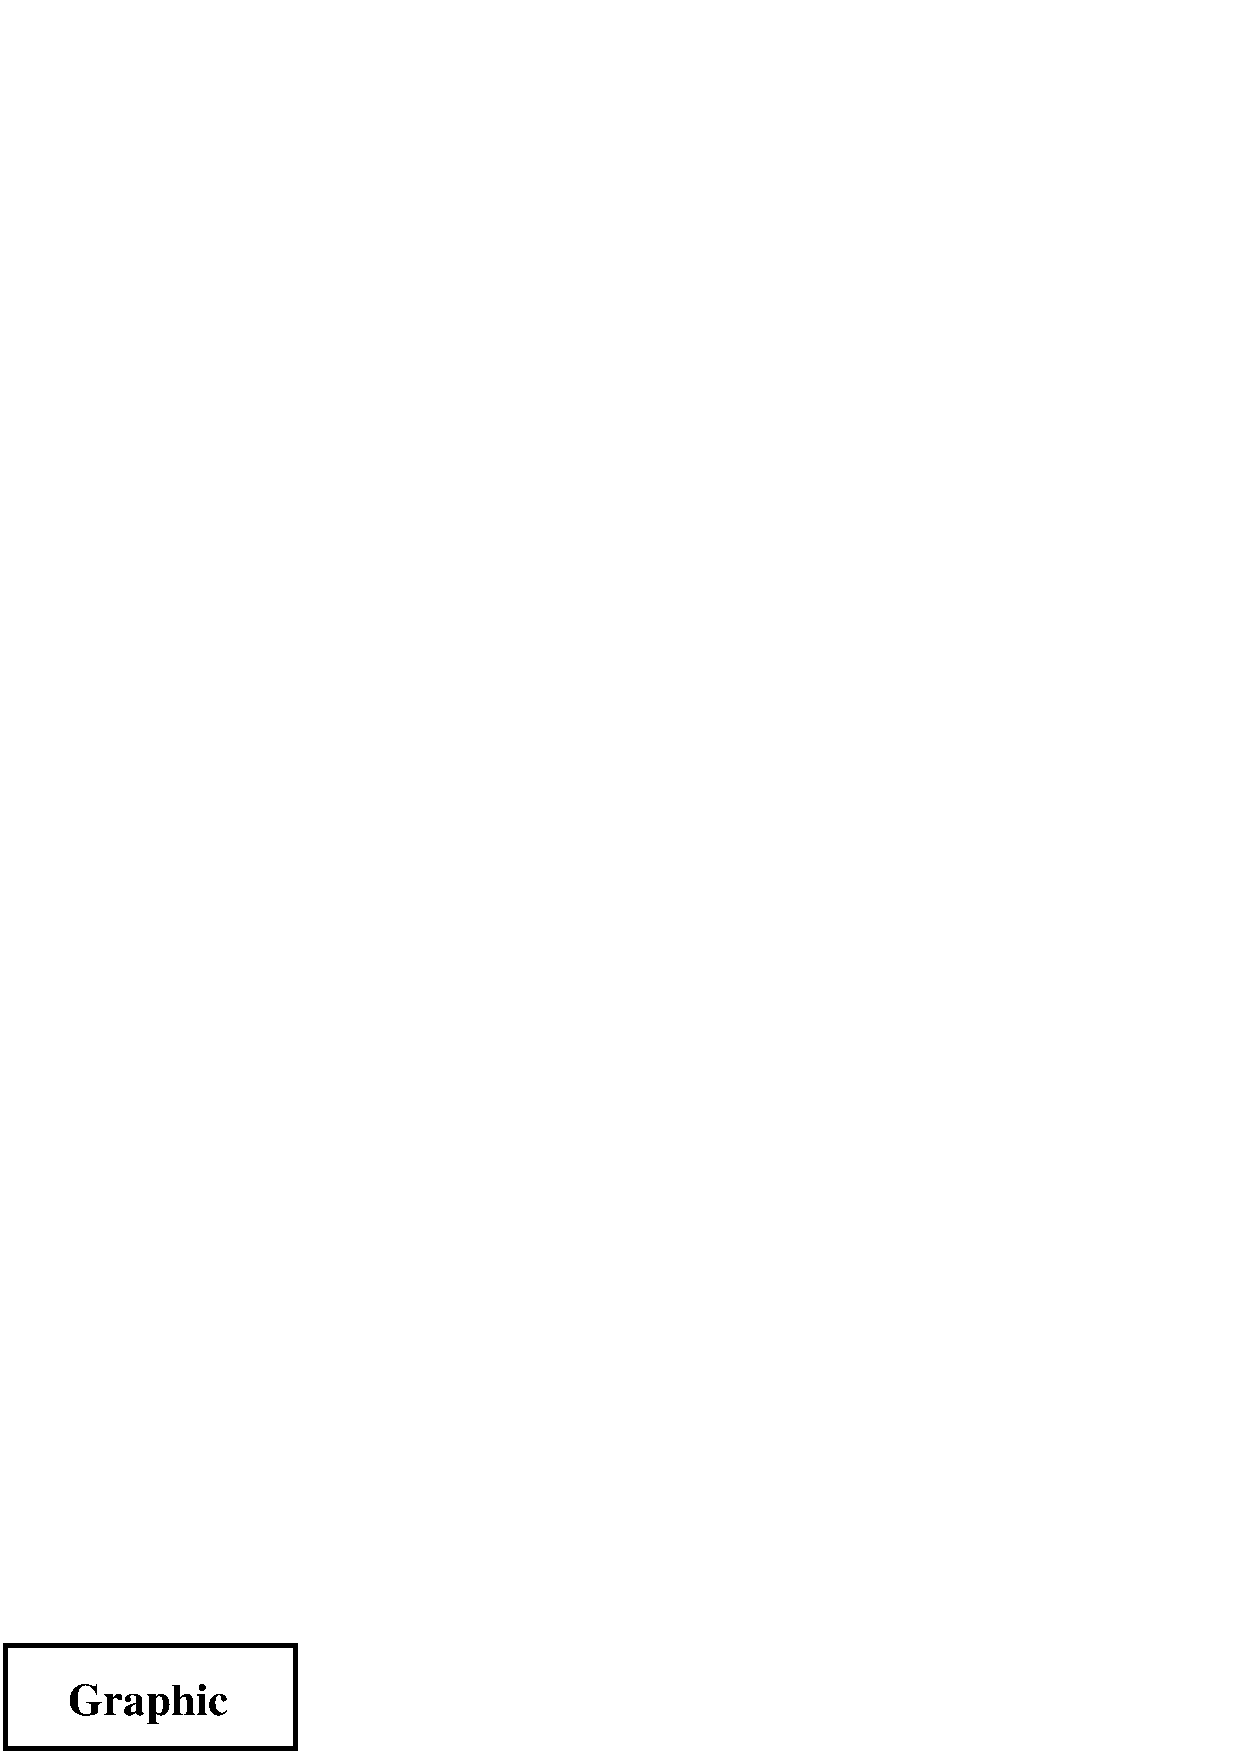
\includegraphics[width=2cm]{graphic}
	\end{minipage}%
	\hspace{1cm}%
	%%----start of second figure graphics----
	\begin{minipage}[b]{.4\linewidth}
		\centering
		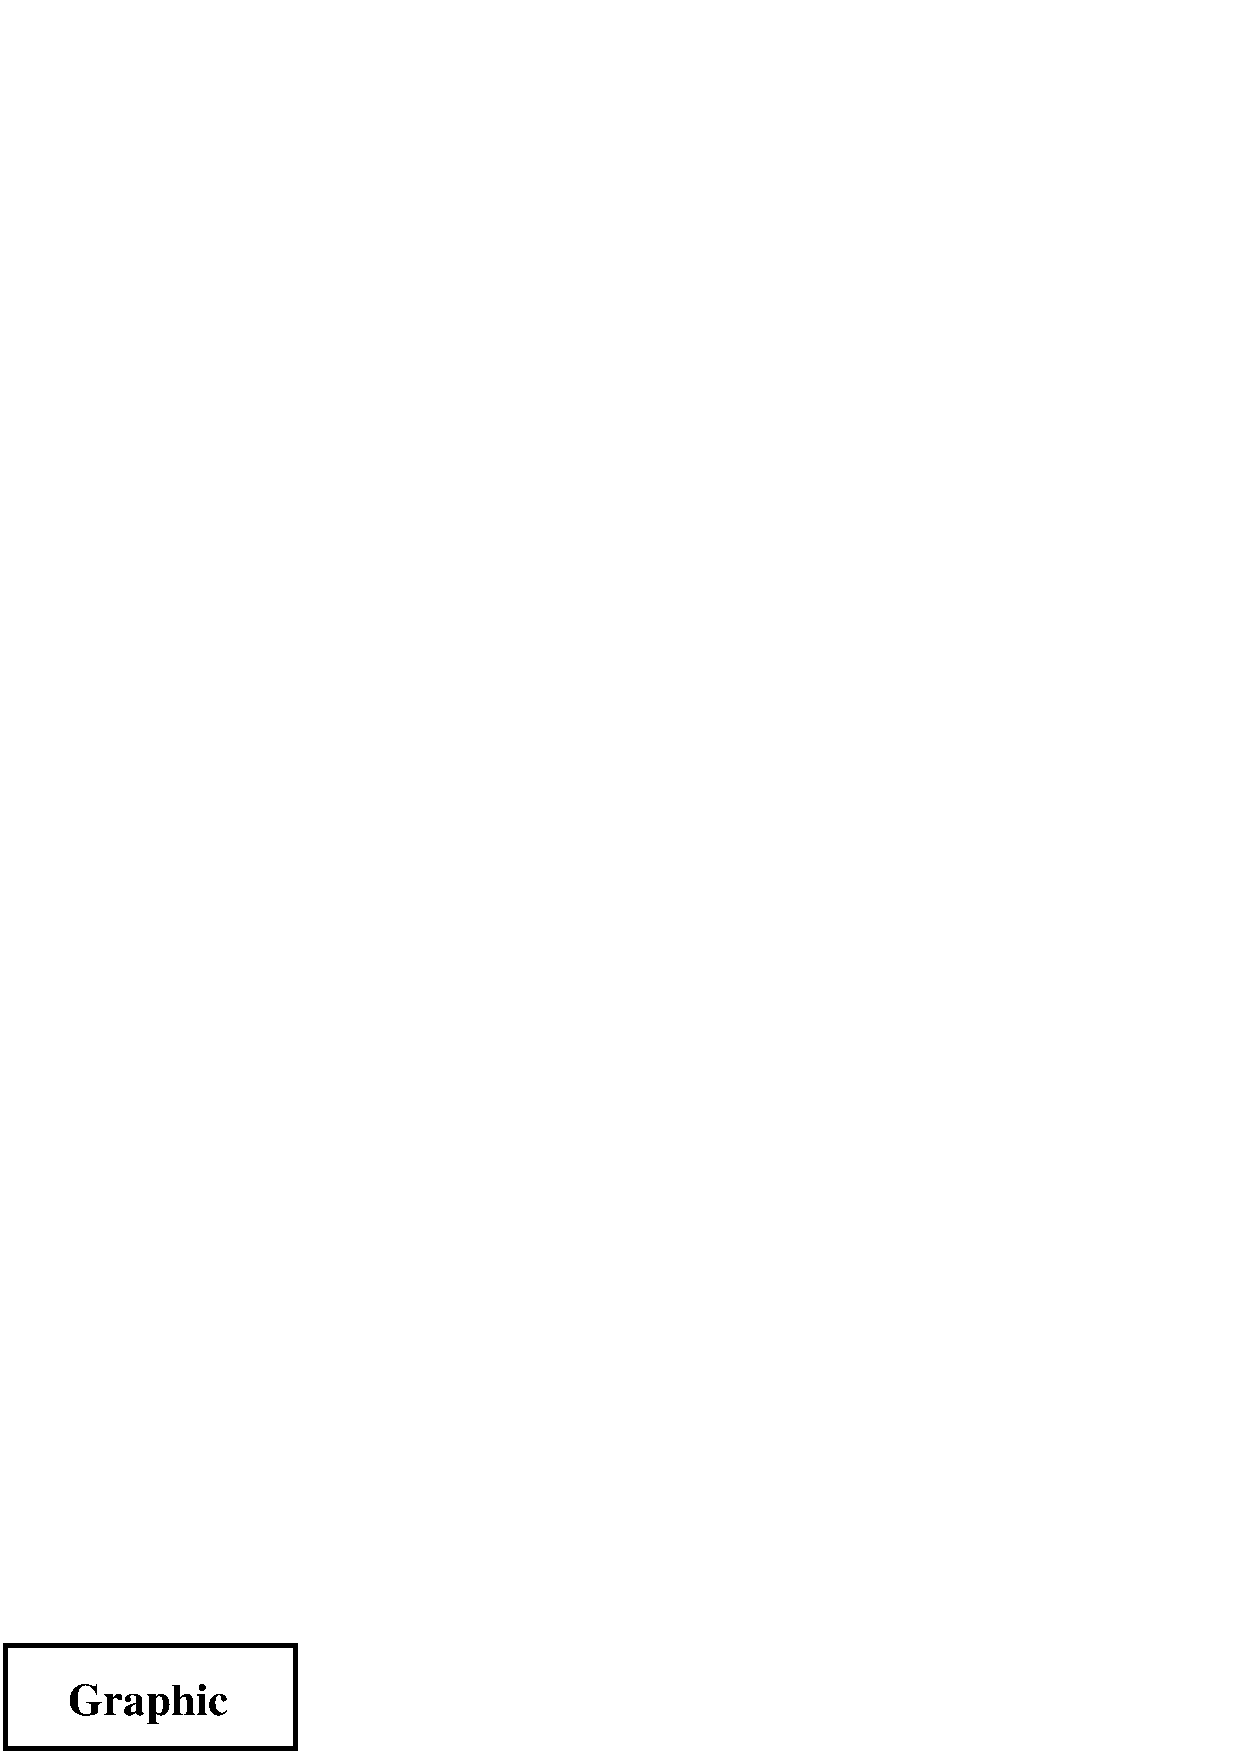
\includegraphics[width=2cm,angle=-30]{graphic}
	\end{minipage}\\[-10pt]
	%%----start of first figure caption----
	\begin{minipage}[t]{.4\linewidth}
		\caption{Box with a Long Caption}
	\end{minipage}%
	\hspace{1cm}%
	%%----start of second figure caption----
	\begin{minipage}[t]{.4\linewidth}
		\caption{Rotated Box}
	\end{minipage}%
\end{figure}
\end{lstlisting}
生成的图~\ref{fig:mininonrot:a}~和~\ref{fig:minirot:a}~中,
图形的基线和标题的第一行分别对齐。

\begin{figure}
	\centering
	%%----start of first figure graphics----
	\begin{minipage}[b]{.4\linewidth}
		\centering
		\resizebox{2cm}{!}{\usebox{\boxgraphic}}
	\end{minipage}%
	\hspace{1cm}%
	%%----start of second figure graphics----
	\begin{minipage}[b]{.4\linewidth}
		\centering
		\rotatebox{-30}{\resizebox{2cm}{!}{\usebox{\boxgraphic}}}
	\end{minipage}\\[-10pt]
	%%----start of first figure caption----
	\begin{minipage}[t]{.4\linewidth}
		\caption{Box with a Long Caption}\label{fig:mininonrot:a}
	\end{minipage}%
	\hspace{1cm}%
	%%----start of second figure caption----
	\begin{minipage}[t]{.4\linewidth}
		\caption{Rotated Box}\label{fig:minirot:a}
	\end{minipage}%
\end{figure}

在这个例子中,需要注意以下几点:
\begin{itemize}
	\item 在最后一幅图后面用 \cmd{\cmd{}} 来断行,
	\cmd{\cmd{}} 的参数项 \opt{[-10pt]} 使得图形与标题之间的距离比当前行距减少10\pt 。
	这样做是让图形和标题更接近些,用户也可自己选用合适的值。
	\item 包含图形的小页使用 \opt{[b]} 选项,使得它们的参考点为其最后一行的基线。
	\item 包含标题小页使用 \opt{[t]} 选项,使得它们的参考点为其第一行的基线,这样使得标题的顶行对齐。
	\item 任何一个 \cmd{label} 命令都必须和它相应的 \cmd{caption} 命令在同一个小页中。
\end{itemize}


\section{图形与表格的平行排列}\label{sec:figuretable}

在第~\ref{sec:sidebyside} 节中,
在一个 \env{figure} 环境中使用多个 \cmd{caption} 命令可以得到并列的多个图形。
同样地,在一个 \env{table} 环境中使用多个 \cmd{caption} 命令可以得到并列的表格。

第~\ref{sec:nonfloat} 节介绍的 \cmd{captionof} 命令可以将表格放在图形旁边。
例如下面的命令:
\begin{lstlisting}
\begin{figure}[htb]
	\begin{minipage}[b]{0.5\linewidth}
		\centering
		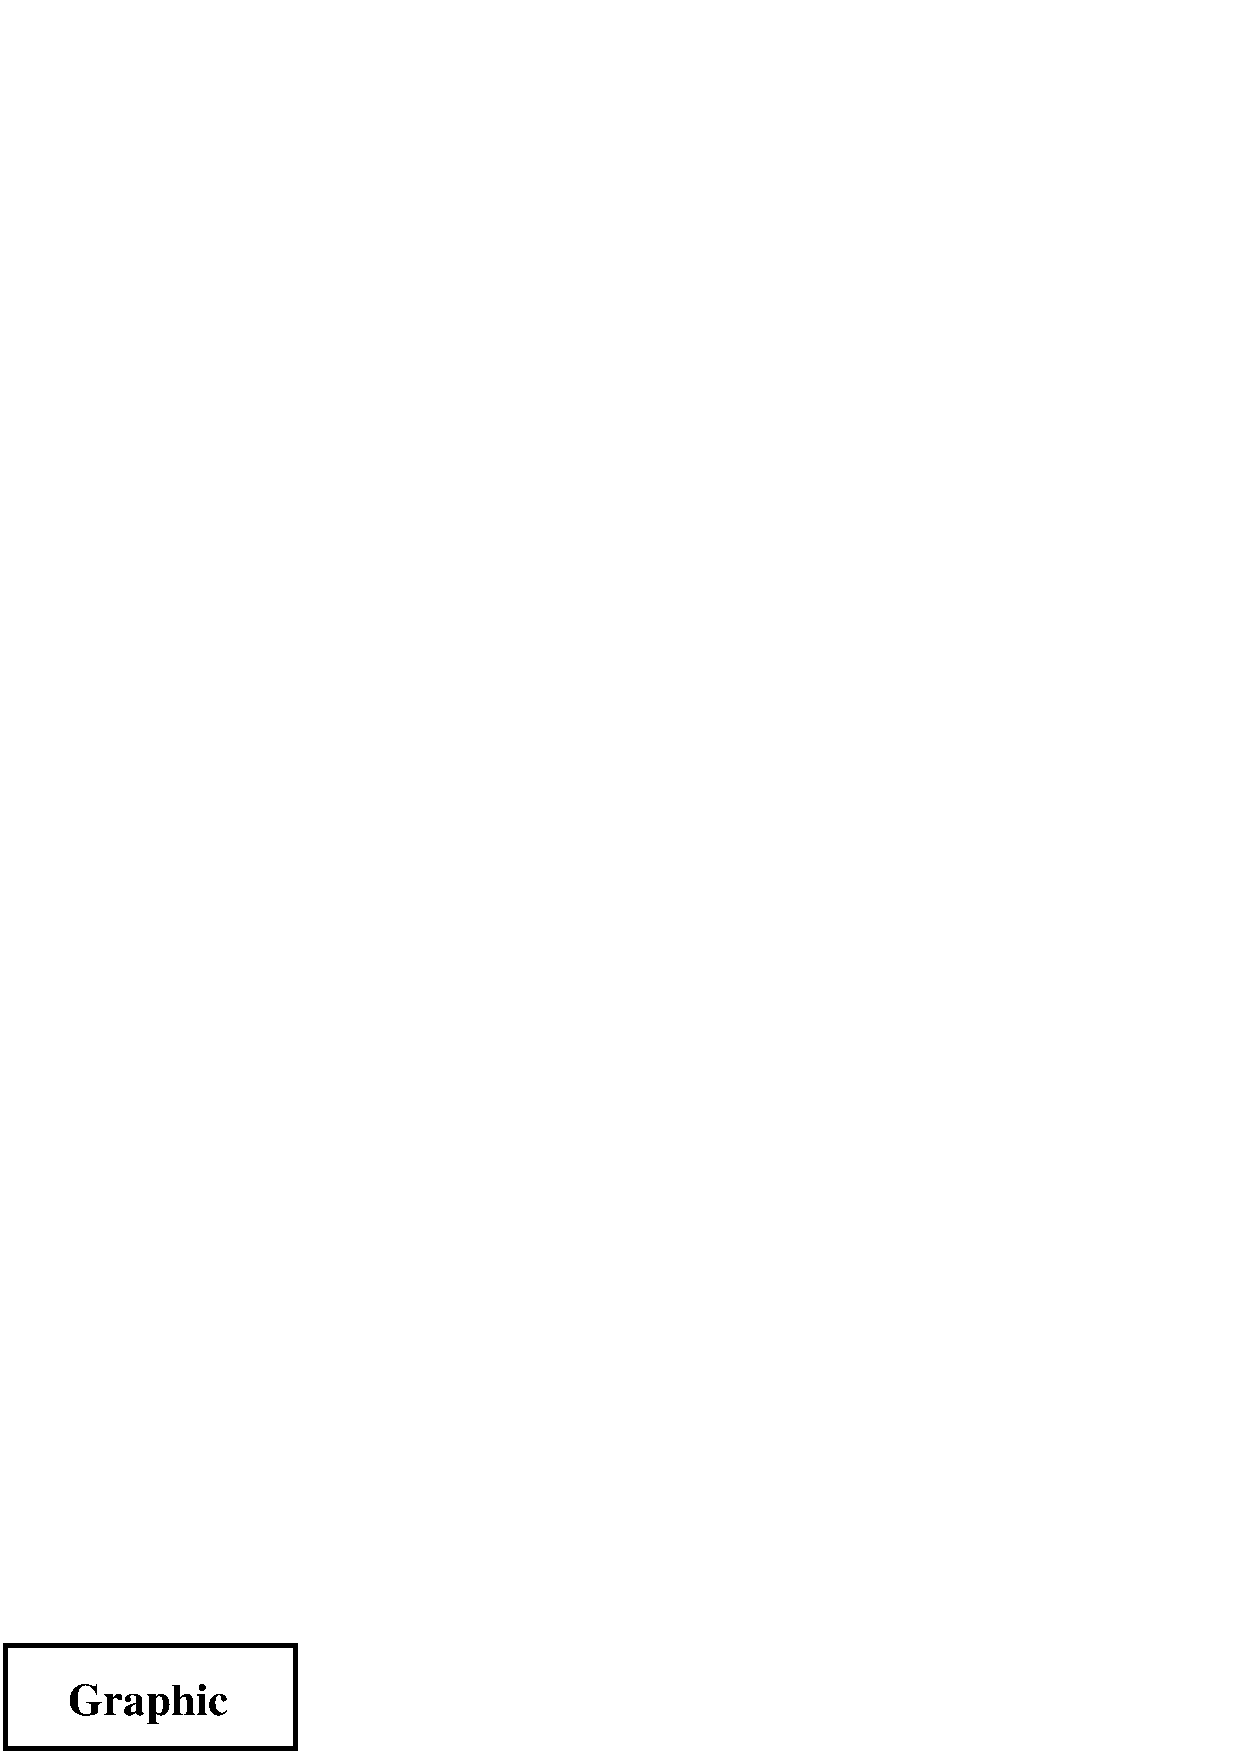
\includegraphics[width=0.8\linewidth]{graphic}
		\caption{This is a Figure by a Table}
		\label{fig:by:table}
	\end{minipage}%
	\begin{minipage}[b]{0.5\linewidth}
		\centering
		\begin{tabular}{|c|c|} \hline
			Day & Data \\ \hline\hline
			Monday & 14.6 \\
			Tuesday & 14.3 \\
			Wednesday & 14.2 \\
			Thursday & 14.5 \\
			Friday & 14.9 \\ \hline
		\end{tabular}
		\captionof{table}{This is a Table by a Figure}
		\label{table:by:fig}
	\end{minipage}
\end{figure}
\end{lstlisting}
使用一个 \env{figure} 环境创建图~\ref{fig:by:table} 和 表~\ref{tab:by:fig}。

\begin{figure}[htb]
	\begin{minipage}[b]{0.5\linewidth}
		\centering
		\resizebox{0.8\linewidth}{!}{\usebox{\boxgraphic}}
		\caption{This is a Figure by a Table}
		\label{fig:by:table}
	\end{minipage}%
	\begin{minipage}[b]{0.5\linewidth}
		\centering
		\begin{tabular}{|c|c|} \hline
			Day & Data \\ \hline\hline
			Monday & 14.6 \\
			Tuesday & 14.3 \\
			Wednesday & 14.2 \\
			Thursday & 14.5 \\
			Friday & 14.9 \\ \hline
		\end{tabular}
		\captionof{table}{This is a Table by a Figure}
		\label{tab:by:fig}
	\end{minipage}
\end{figure}

因为 \LaTeX{} 允许图形的浮动不必考虑其前后表格的顺序,
所以在 \env{figure} 环境中使用
\begin{lstlisting}
\captionof{table}{...}
\end{lstlisting}
可能会将该表格放在未处理的表格之前。
类似地,在 \env{table} 环境中使用
\begin{lstlisting}
\captionof{figure}{...}
\end{lstlisting}
可能会将该图形放在未处理的图形之前。
如果不希望这样,
可以在 \env{figure} 环境之前使用 \cmd{FloatBarrier} 或者 \cmd{clearpage} 命令清除未处理的浮动体
(参见第~\ref{ssec:unprocessfig} 节)。


\section{堆叠的图形和子图}\label{sec:stackfigs}

第~\ref{sec:sidebyside}~节介绍了一系列方法创建并列图形。
这些方法的原理都是将对象(图形、小页、子浮动体等)依次排列在一条直线上。
当使用 \cmd{\cmd{}} 显式断行时,相同的方法也可以生成堆叠的图形。
此外还可以通过 \cmd{\cmd{}} 命令的可选参数(例如 \cmd{\cmd{}}\opt{[20pt]})指定竖直间距。

\subsection{堆叠的图形}\label{ssec:stackfigs}

第~\ref{sec:sidebyside}~节介绍了如何创建并列图形。
本节的内容表明,添加断行可以生成多行图形。
例如下列代码
\begin{lstlisting}
\begin{figure}[htbp]
	\centering
	%%----start of first figure----
	\begin{minipage}[t]{0.25\linewidth}
		\centering
		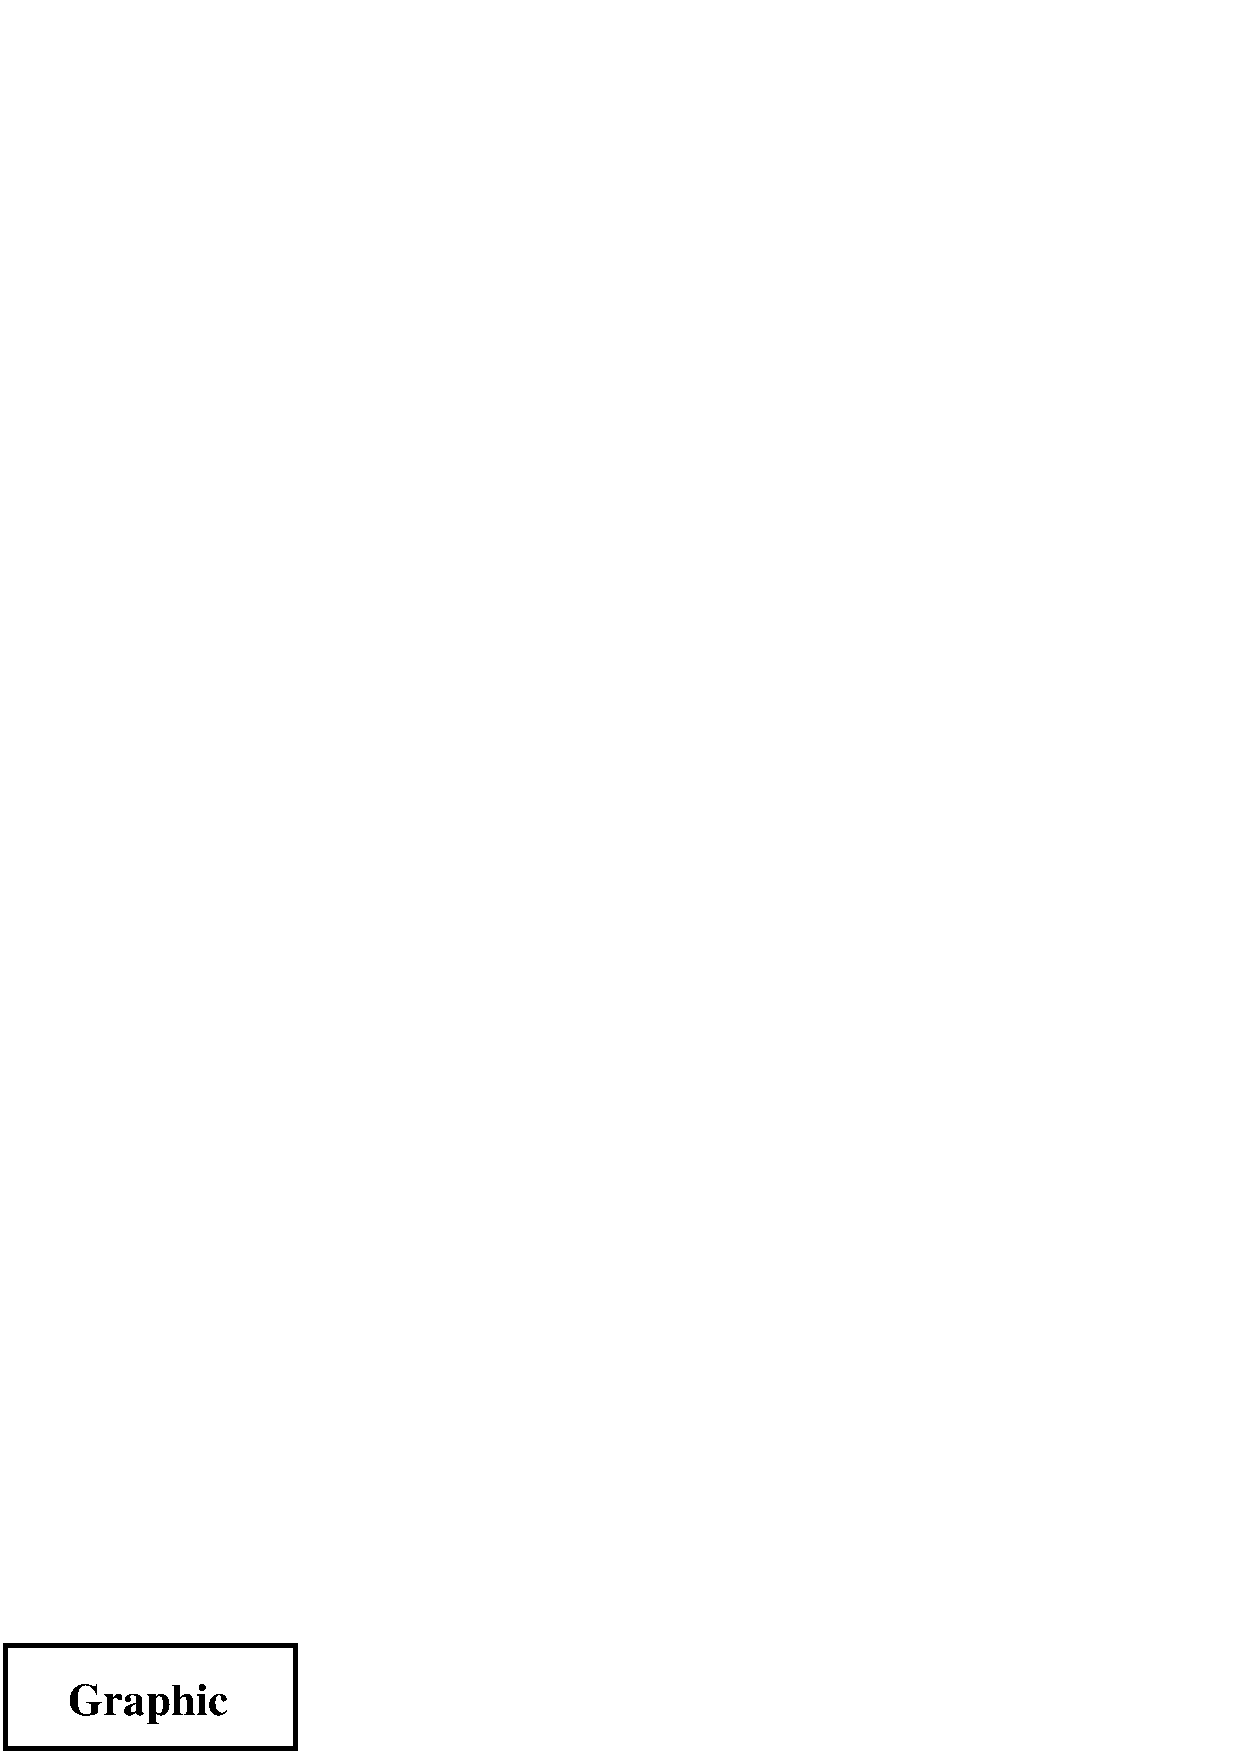
\includegraphics[width=\linewidth]{graphic}
		\caption{First Stacked Figure}
		\label{fig:stacked:first}
	\end{minipage}%
	\hspace{1cm}%
	%%----start of second figure----
	\begin{minipage}[t]{0.25\linewidth}
		\centering
		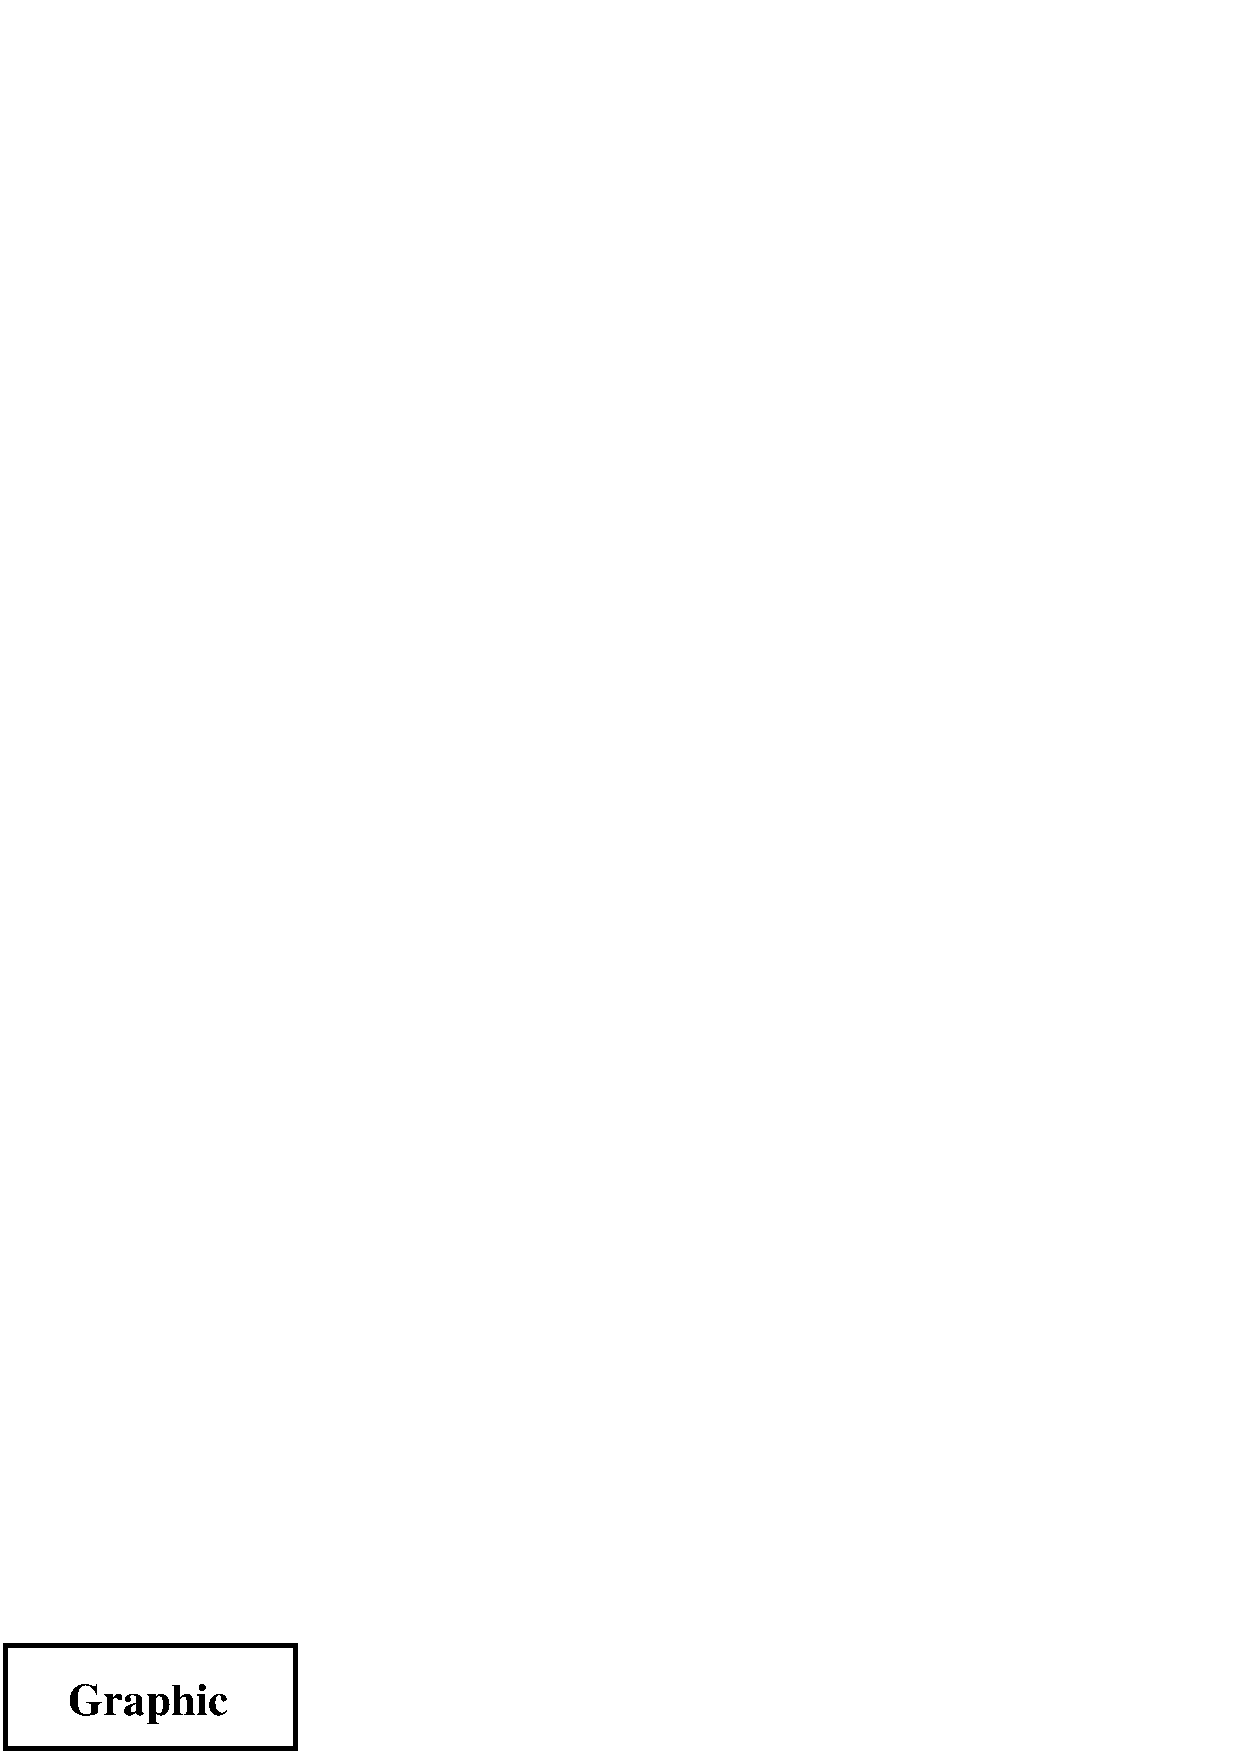
\includegraphics[width=\linewidth]{graphic}
		\caption{Second Stacked Figure}
		\label{fig:stacked:second}
	\end{minipage}\\[20pt]
	%%----start of third figure----
	\begin{minipage}[t]{0.25\linewidth}
		\centering
		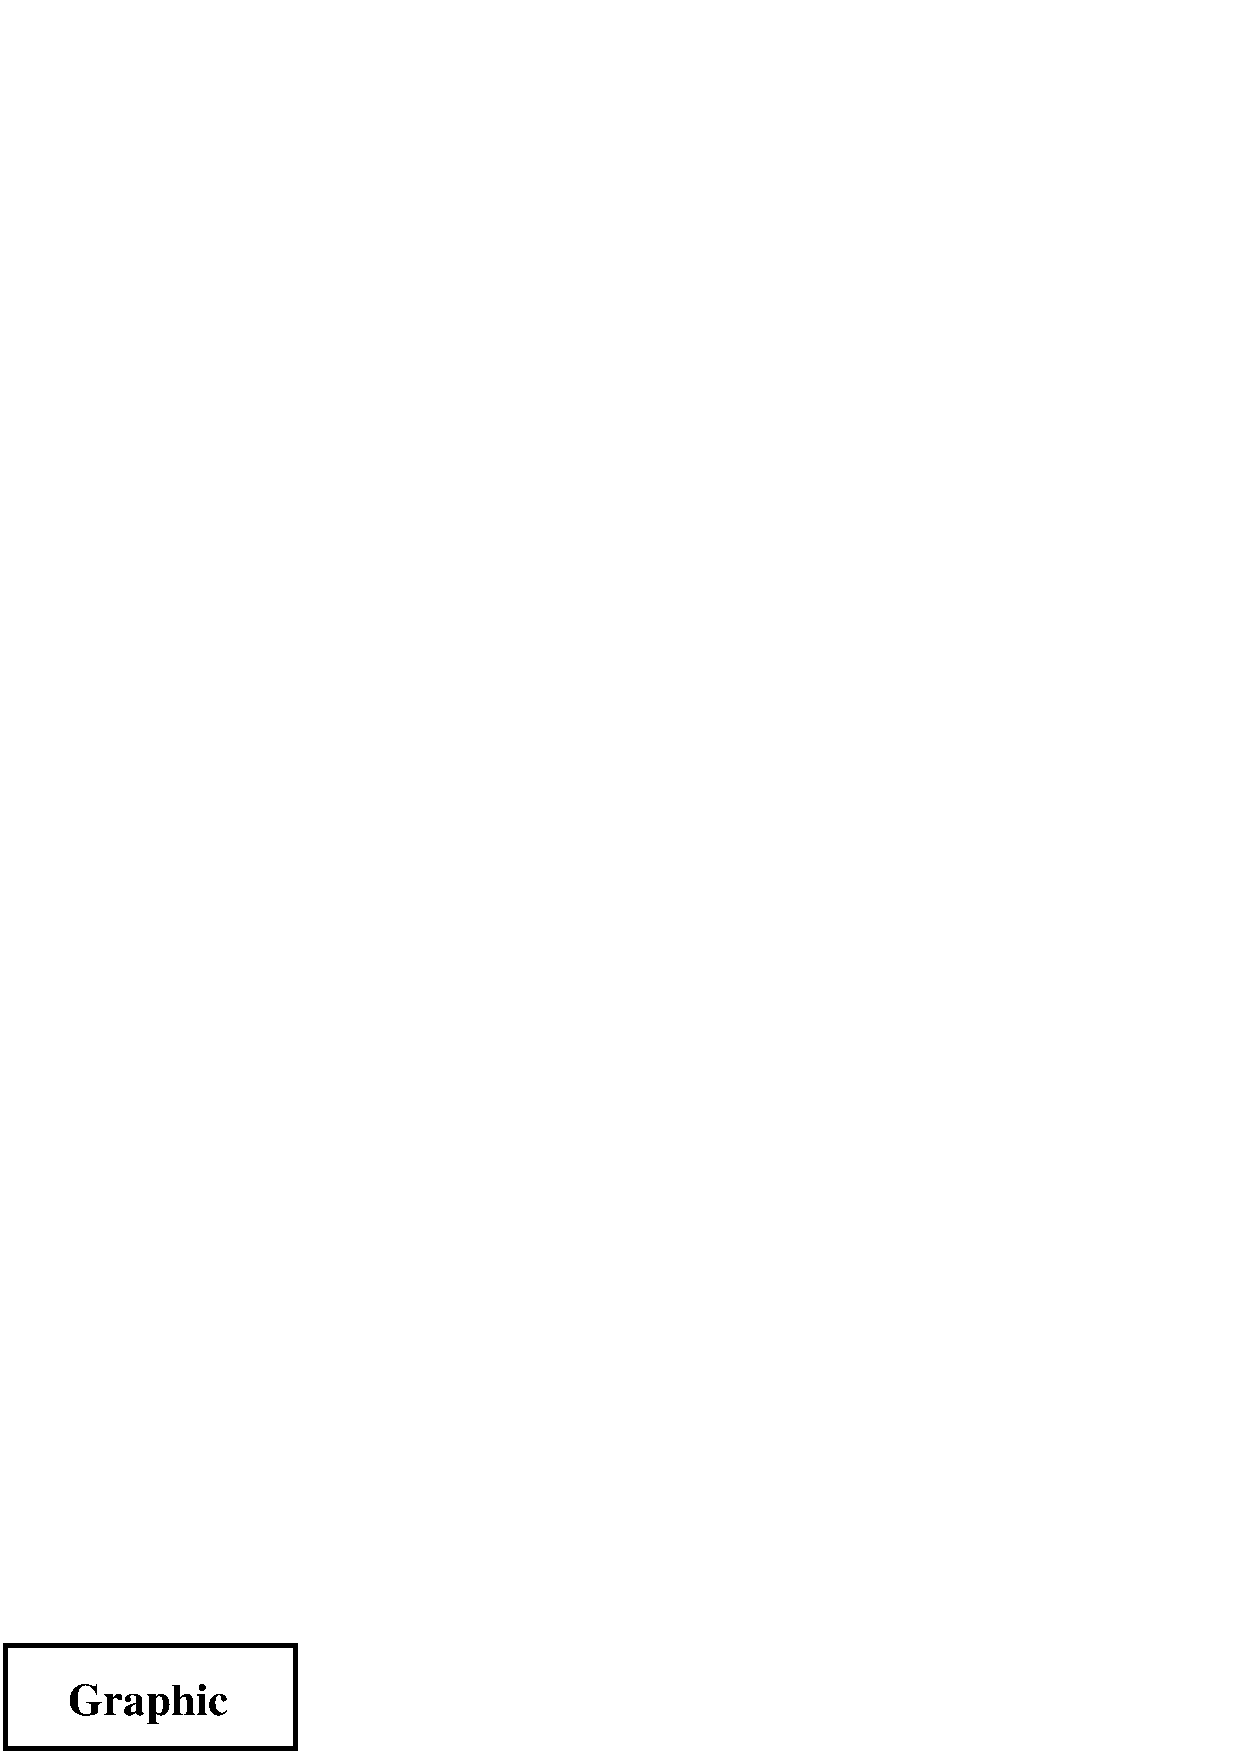
\includegraphics[width=\linewidth]{graphic}
		\caption{Third Stacked Figure}
		\label{fig:stacked:third}
	\end{minipage}%
	\hspace{1cm}%
	%%----start of fourth figure----
	\begin{minipage}[t]{0.25\linewidth}
		\centering
		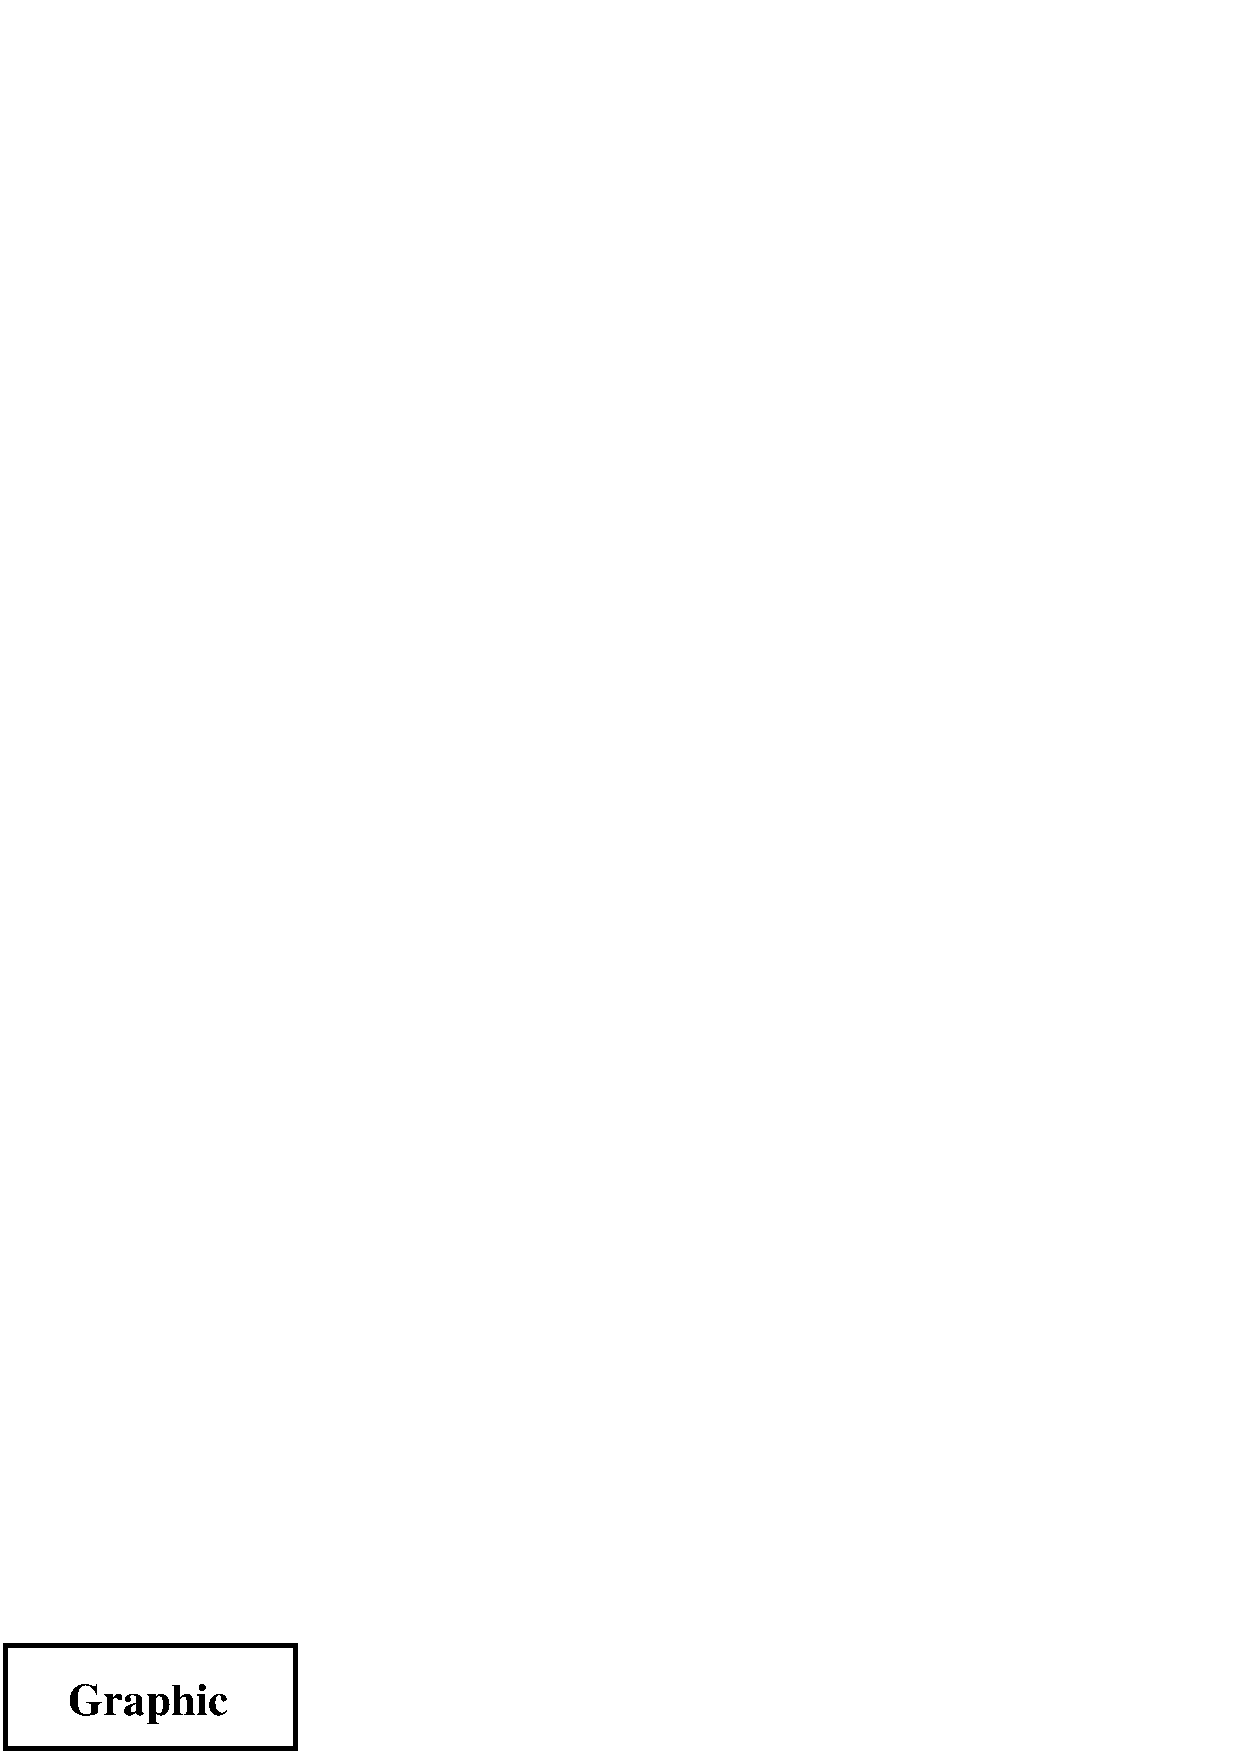
\includegraphics[width=\linewidth]{graphic}
		\caption{Fourth Stacked Figure}
		\label{fig:stacked:fourth}
	\end{minipage}%
	\hspace{1cm}%
	%%----start of fifth figure----
	\begin{minipage}[t]{0.25\linewidth}
		\centering
		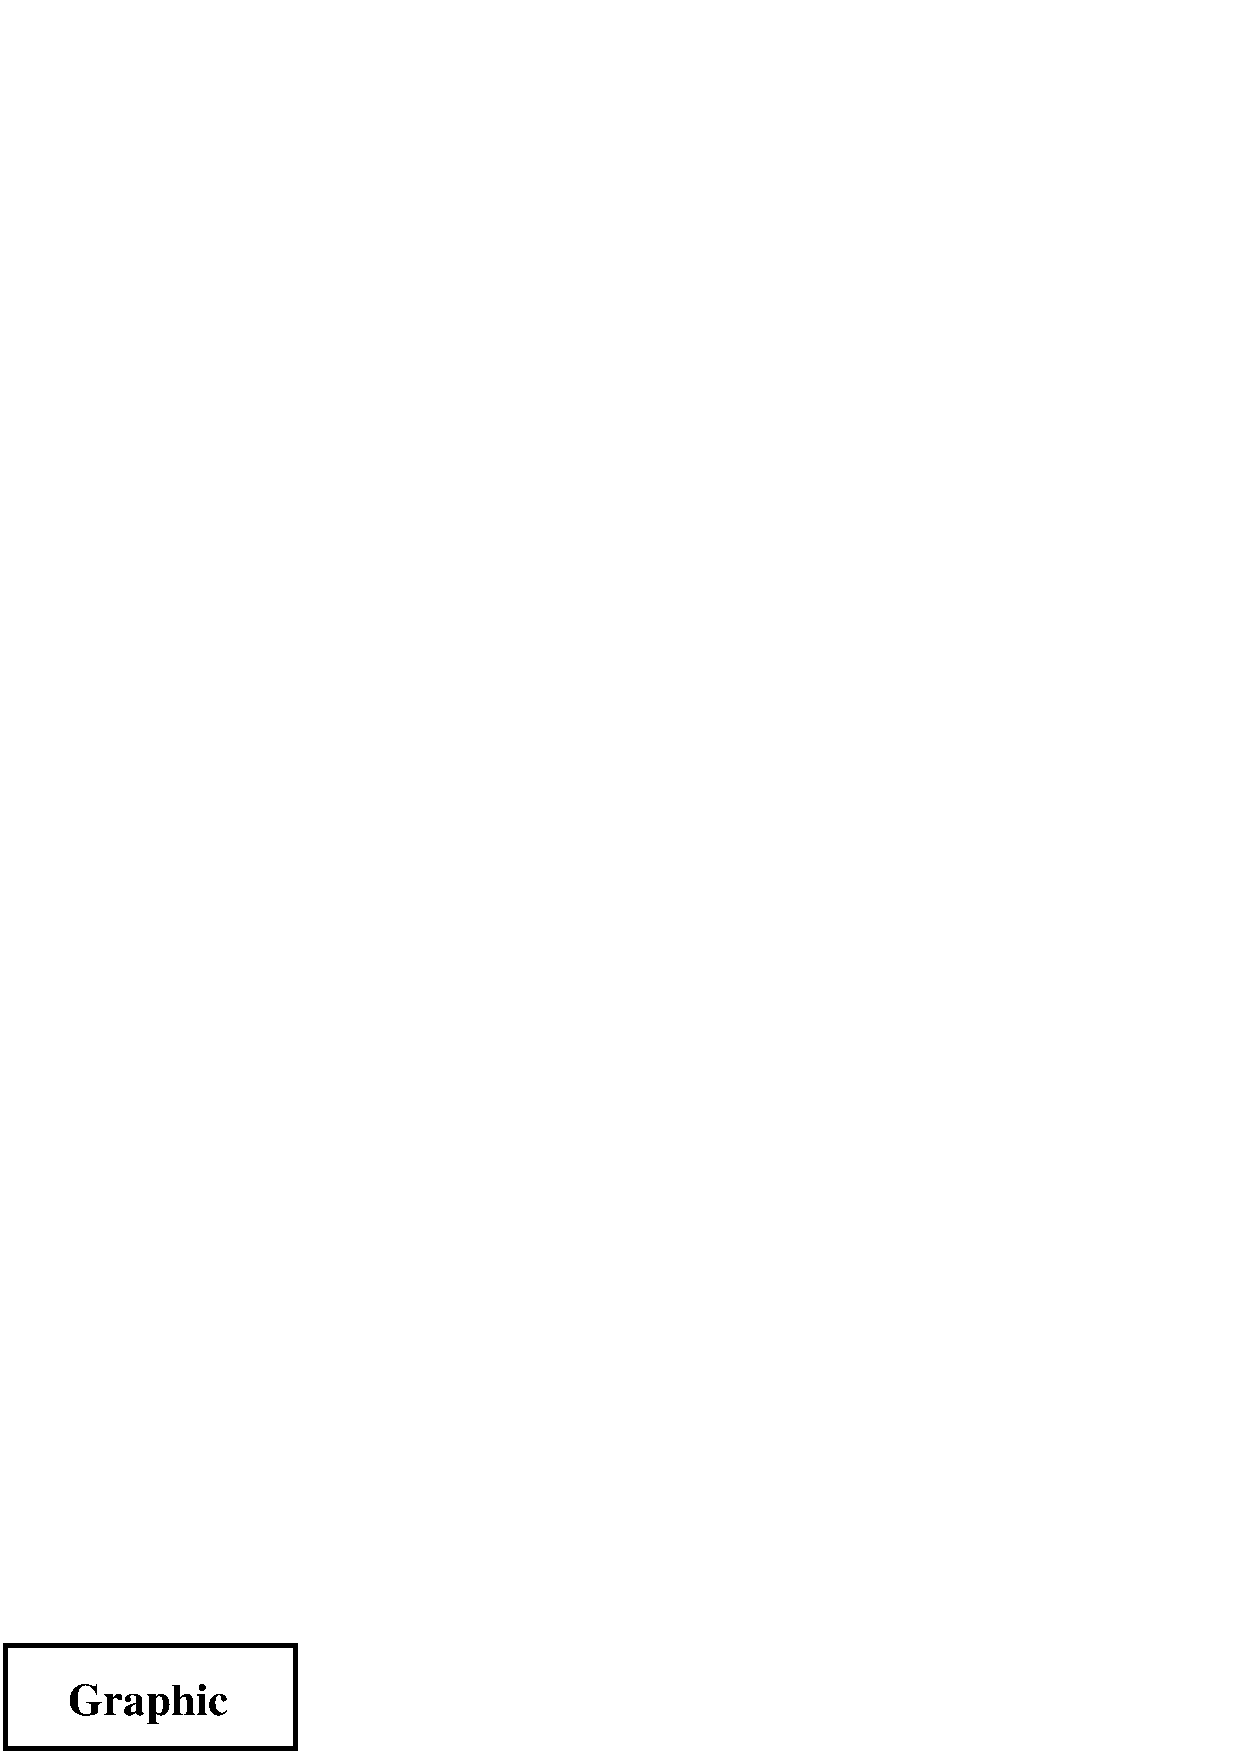
\includegraphics[width=\linewidth]{graphic}
		\caption{Fifth Stacked Figure}
		\label{fig:stacked:fifth}
	\end{minipage}%
\end{figure}
\end{lstlisting}
生成一组图~\ref{fig:stacked:first}--\ref{fig:stacked:fifth}。

\begin{figure}[htbp]
	\centering
	%%----start of first figure----
	\begin{minipage}[t]{0.25\linewidth}
		\centering
		\resizebox{\linewidth}{!}{\usebox{\boxgraphic}}
		\caption{First Stacked Figure}
		\label{fig:stacked:first}
	\end{minipage}%
	\hspace{1cm}%
	%%----start of second figure----
	\begin{minipage}[t]{0.25\linewidth}
		\centering
		\resizebox{\linewidth}{!}{\usebox{\boxgraphic}}
		\caption{Second Stacked Figure}
		\label{fig:stacked:second}
	\end{minipage}\\[20pt]
	%%----start of third figure----
	\begin{minipage}[t]{0.25\linewidth}
		\centering
		\resizebox{\linewidth}{!}{\usebox{\boxgraphic}}
		\caption{Third Stacked Figure}
		\label{fig:stacked:third}
	\end{minipage}%
	\hspace{1cm}%
	%%----start of fourth figure----
	\begin{minipage}[t]{0.25\linewidth}
		\centering
		\resizebox{\linewidth}{!}{\usebox{\boxgraphic}}
		\caption{Fourth Stacked Figure}
		\label{fig:stacked:fourth}
	\end{minipage}%
	\hspace{1cm}%
	%%----start of fifth figure----
	\begin{minipage}[t]{0.25\linewidth}
		\centering
		\resizebox{\linewidth}{!}{\usebox{\boxgraphic}}
		\caption{Fifth Stacked Figure}
		\label{fig:stacked:fifth}
	\end{minipage}%
\end{figure}

\subsection{堆叠的子图}\label{ssec:stackedsubfigs}

第~\ref{ssec:sidesubfigure}~节介绍了如何创建并列的子图。
本节的内容表明,添加断行可以生成多行子图。
例如下列代码

%	%%----start of first subfigure----
%	\subcaptionbox{Small Box with a Long Caption%
%		\label{fig:subfig:a} %% label for first subfigure
%	}{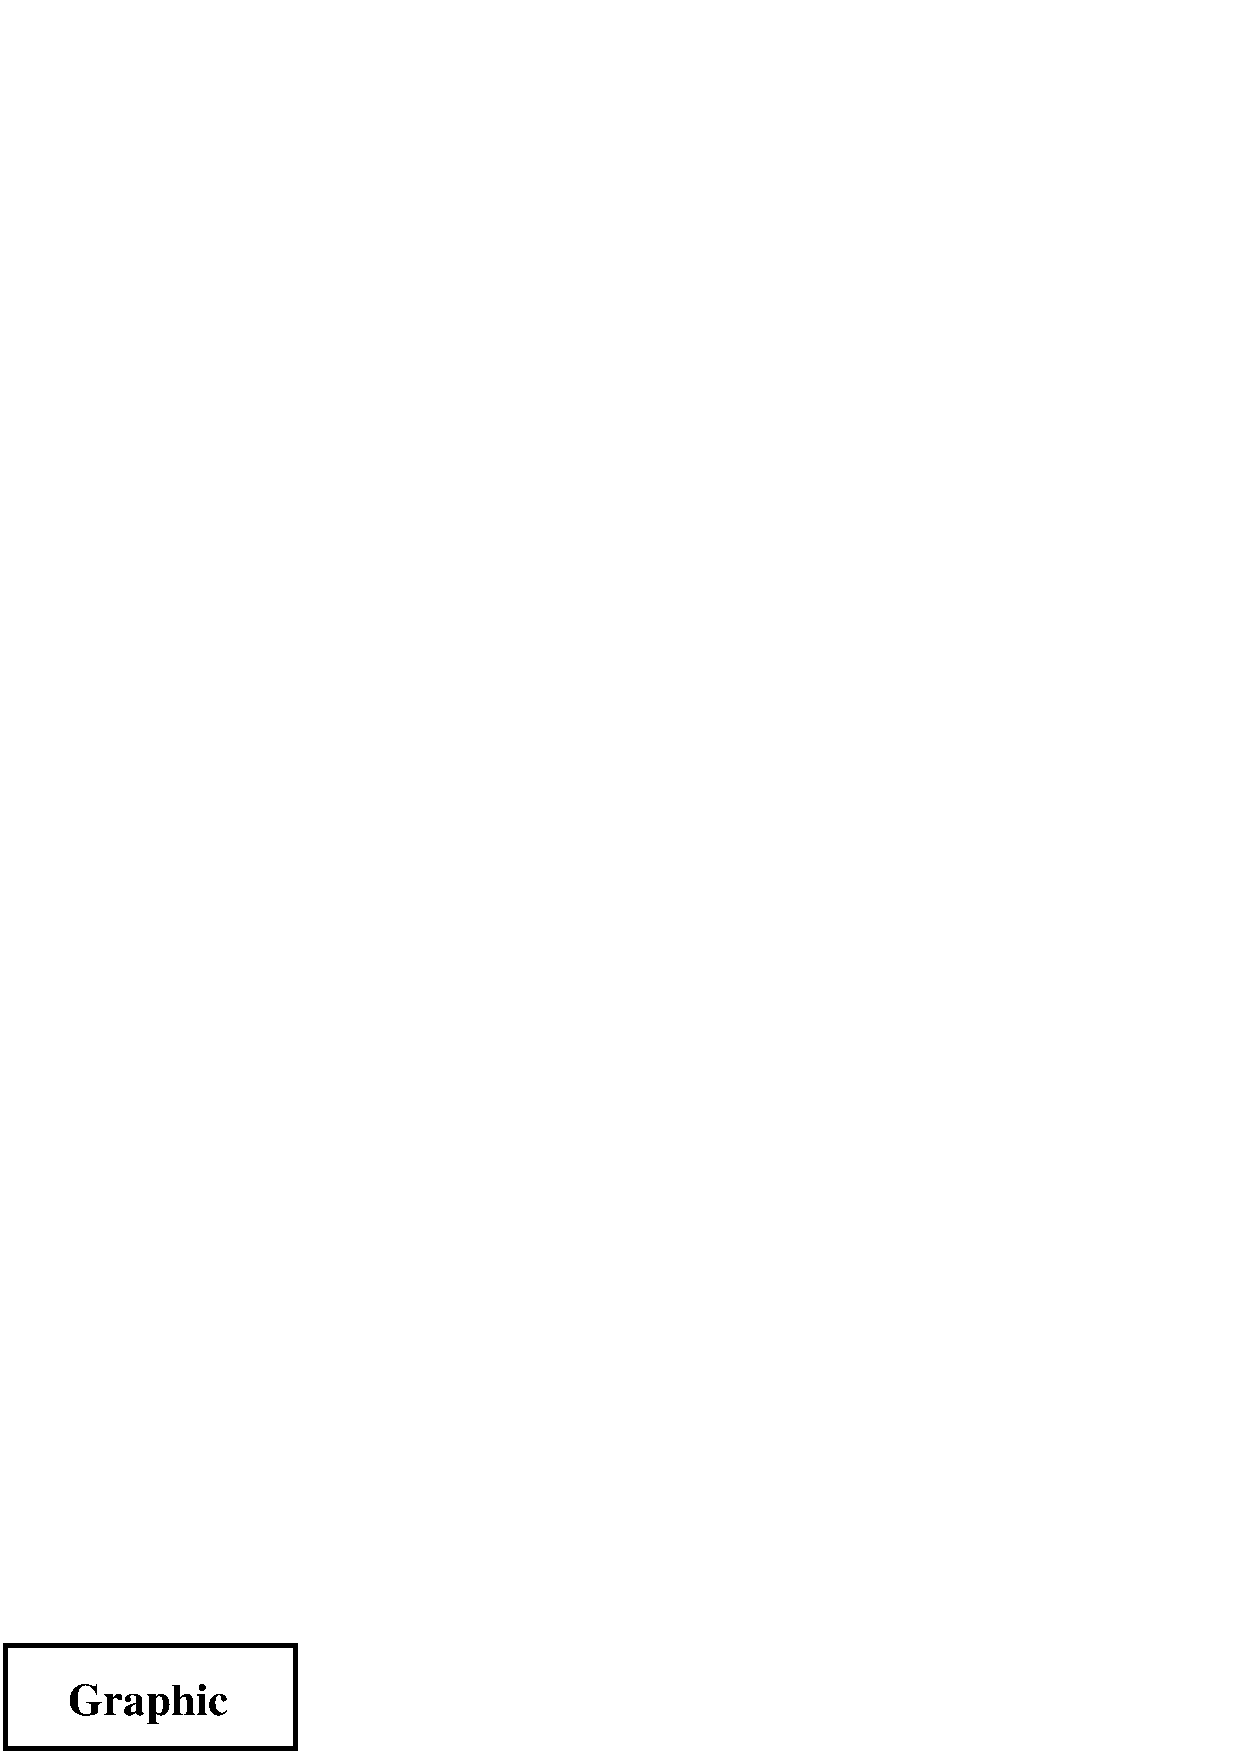
\includegraphics[width=1.1in]{graphic}}

\begin{lstlisting}
\begin{figure}
	\centering
	%%----start of first subfigure----
	% label for first subfigure
	\subcaptionbox{First Subfigure\label{fig:stacksub:a}}%
		{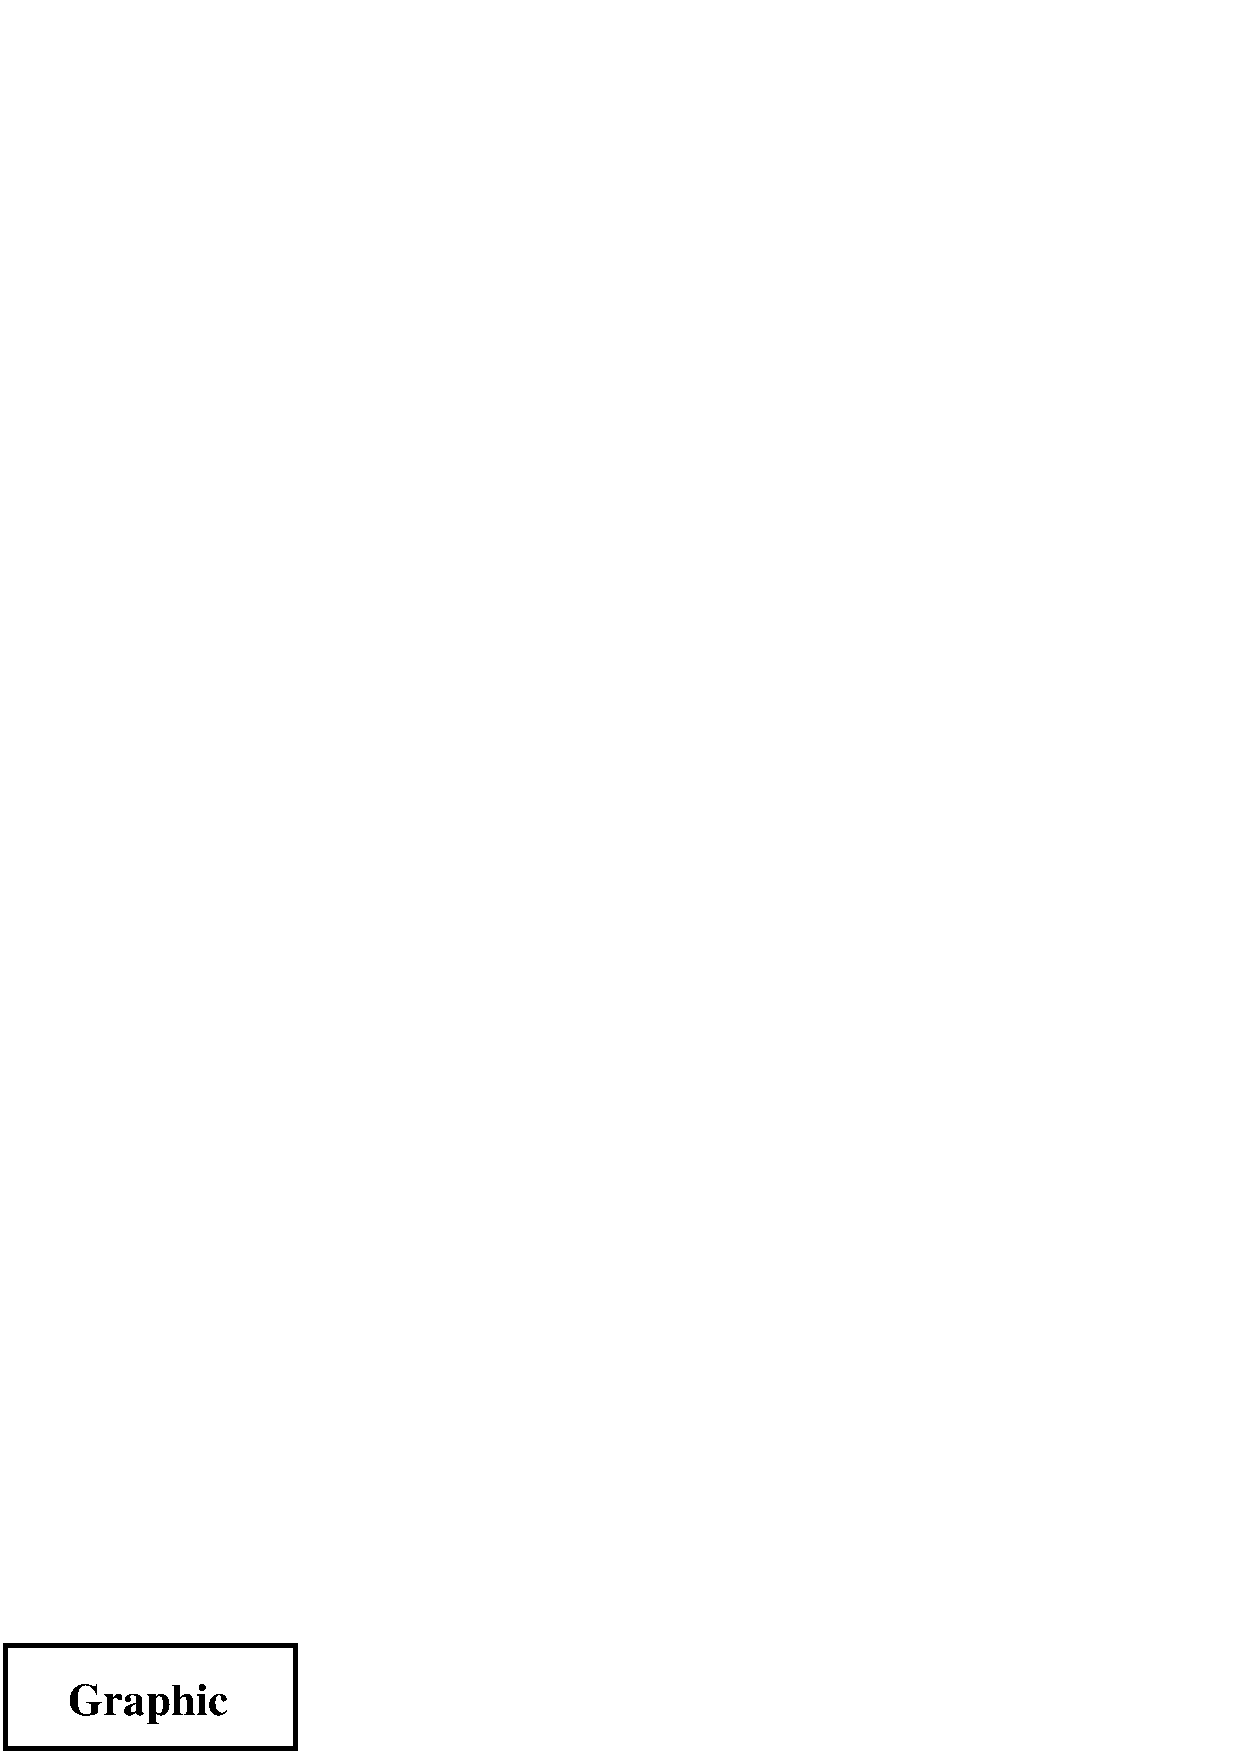
\includegraphics[width=0.25\linewidth]{graphic}}
	\hspace{0.1\linewidth}
	%%----start of second subfigure----
	% label for second subfigure
	\subcaptionbox{Second Subfigure\label{fig:stacksub:b}}%
		{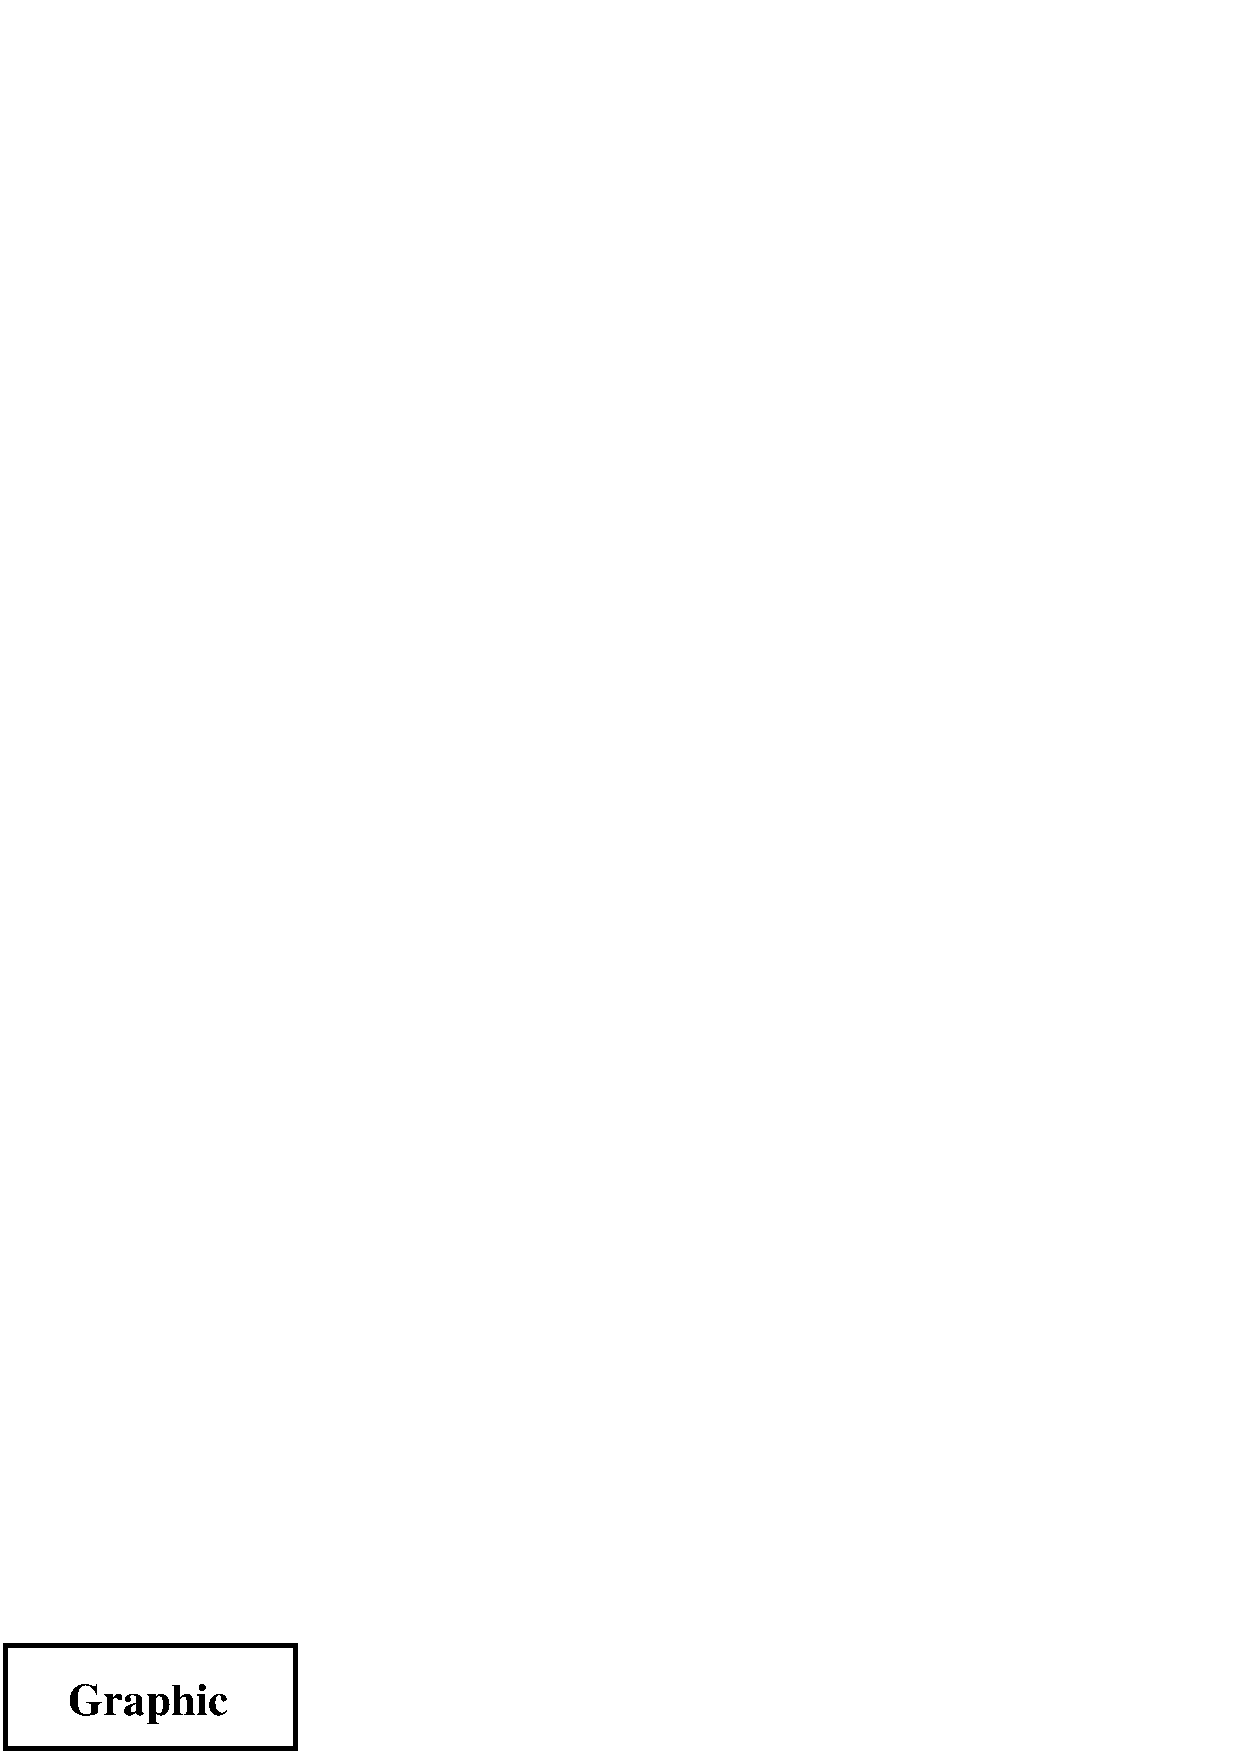
\includegraphics[width=0.25\linewidth]{graphic}}\\[20pt]
	%%----start of third subfigure----
	% label for third subfigure
	\subcaptionbox{Third Subfigure\label{fig:stacksub:c}}%
		{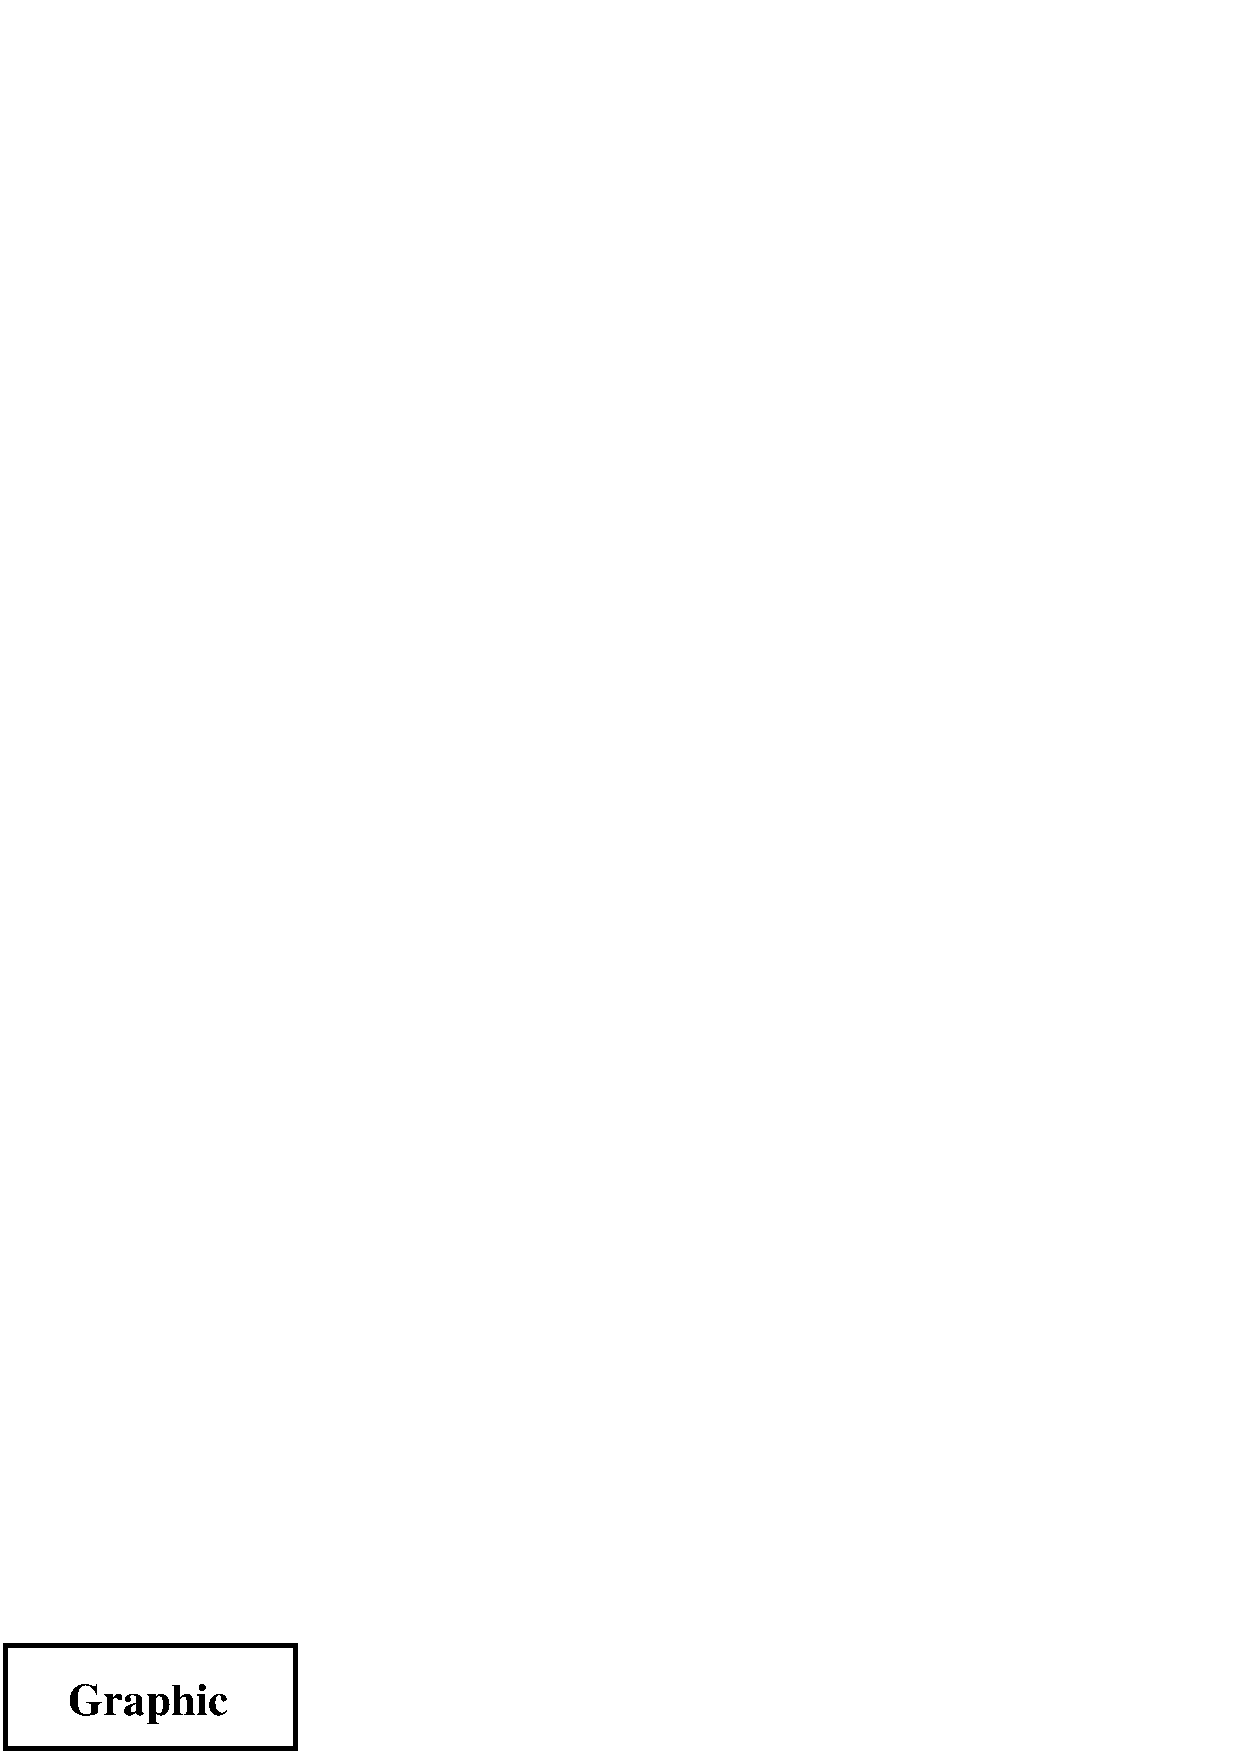
\includegraphics[width=0.25\linewidth]{graphic}}
	\hspace{0.1\linewidth}
	%%----start of fourth subfigure----
	% label for fourth subfigure
	\subcaptionbox{Fourth Subfigure\label{fig:stacksub:d}}%
		{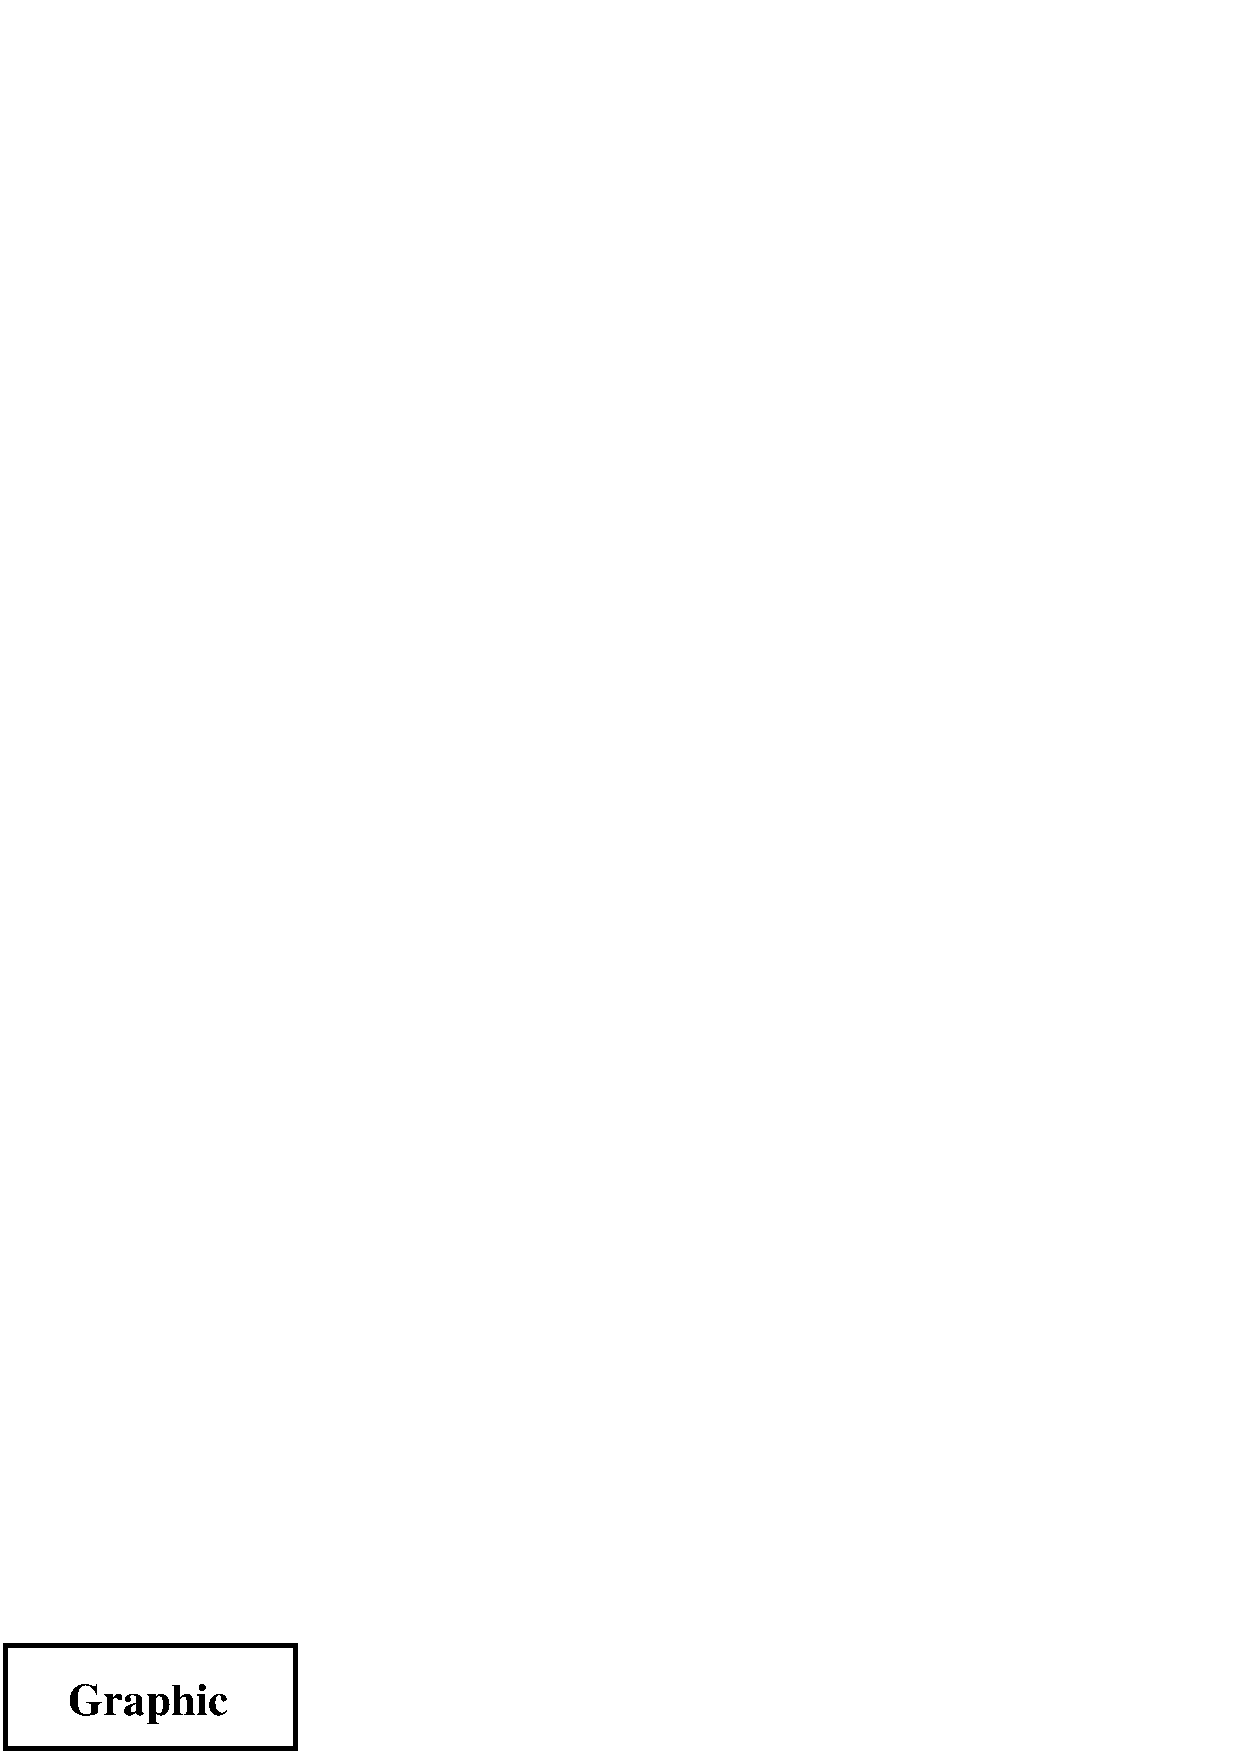
\includegraphics[width=0.25\linewidth]{graphic}}
	\hspace{0.1\linewidth}
	%%----start of fifth subfigure----
	% label for fifth subfigure
	\subcaptionbox{Fifth Subfigure\label{fig:stacksub:e}}%
		{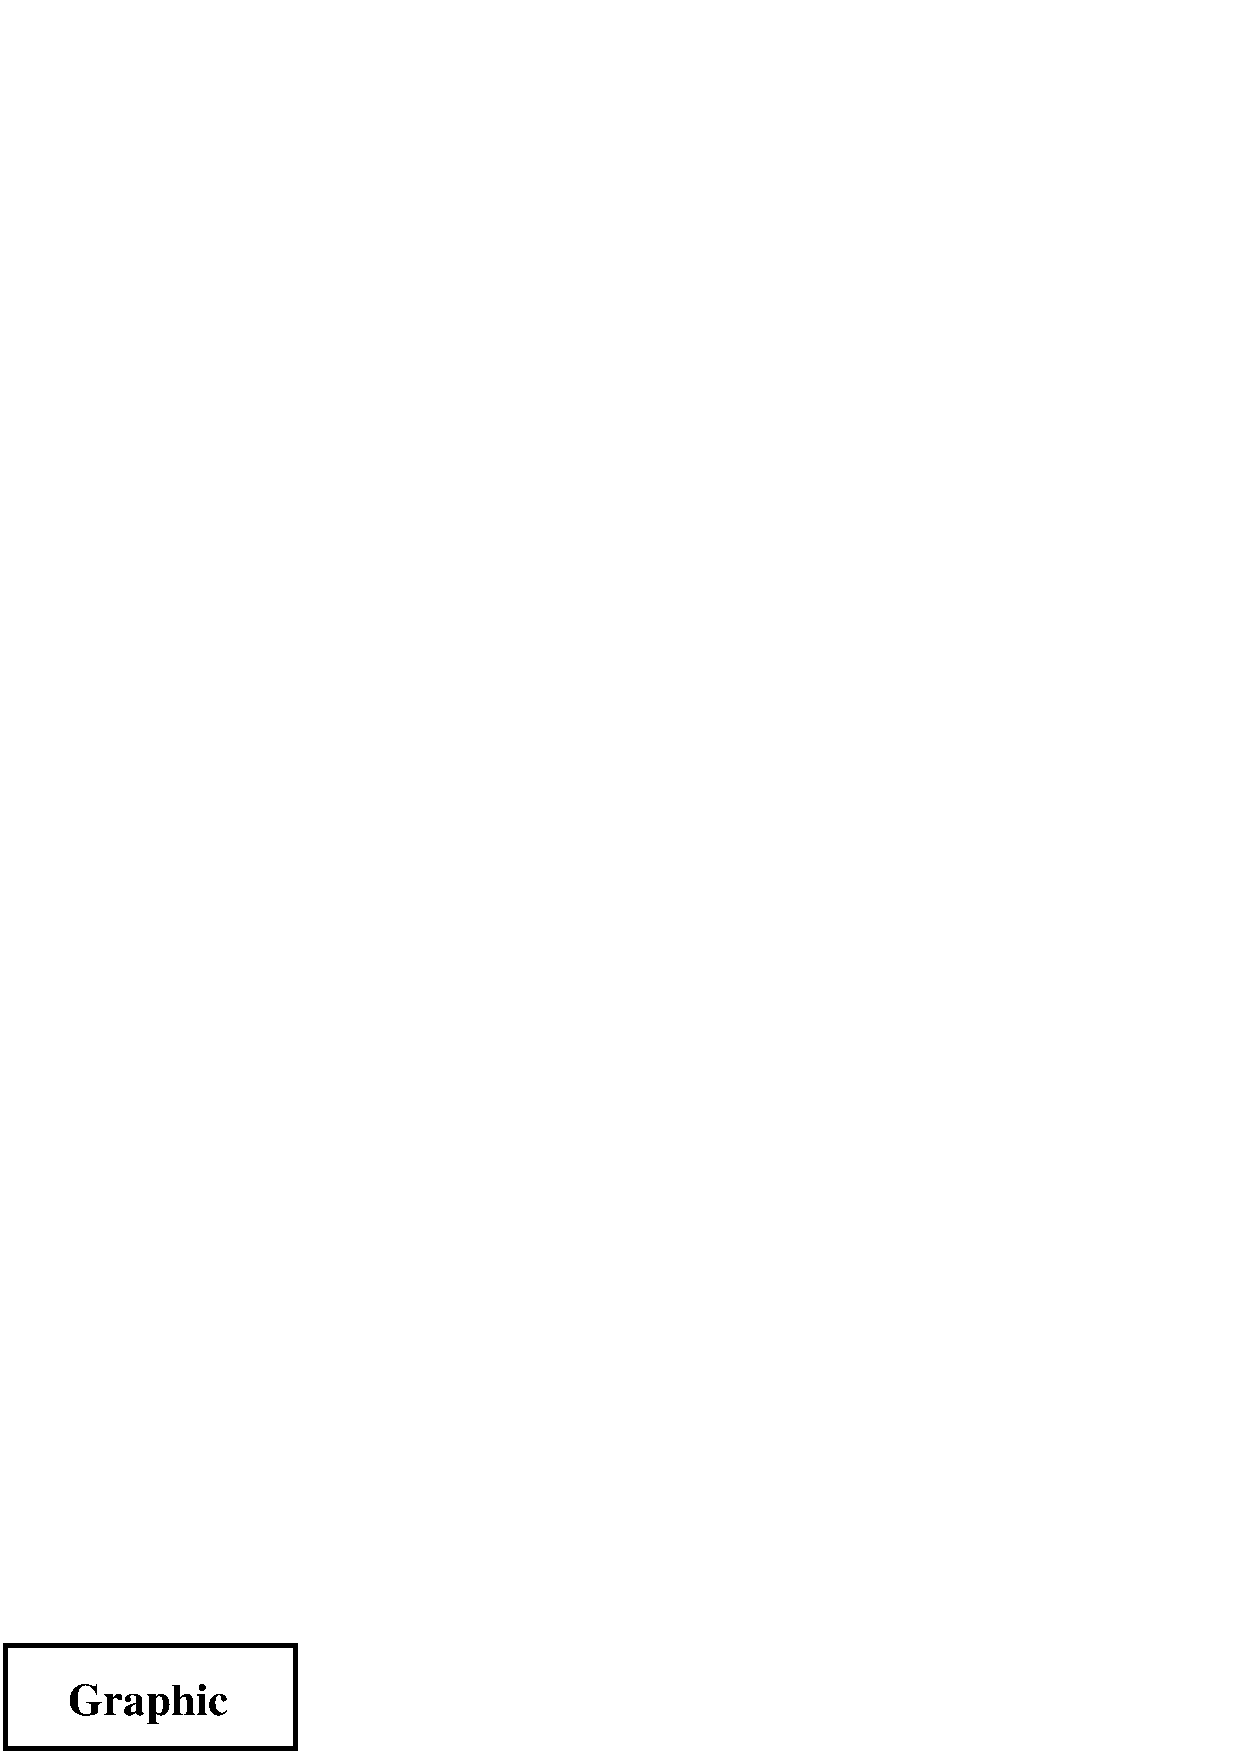
\includegraphics[width=0.25\linewidth]{graphic}}
	\caption{Five Subfigures}
	\label{fig:stacksub} %% label for entire figure
\end{figure}
\end{lstlisting}
生成图~\ref{fig:stacksub}。

\begin{figure}
	\centering
	%%----start of first subfigure----
	\subcaptionbox{First Subfigure\label{fig:stacksub:a}}%% label for first subfigure
		{\resizebox{0.25\linewidth}{!}{\usebox{\boxgraphic}}}
	\hspace{0.1\linewidth}
	%%----start of second subfigure----
	\subcaptionbox{Second Subfigure\label{fig:stacksub:b}}%% label for second subfigure
		{\resizebox{0.25\linewidth}{!}{\usebox{\boxgraphic}}}\\[20pt]
	%%----start of third subfigure----
	\subcaptionbox{Third Subfigure\label{fig:stacksub:c}}%% label for third subfigure
		{\resizebox{0.25\linewidth}{!}{\usebox{\boxgraphic}}}
	\hspace{0.1\linewidth}
	%%----start of fourth subfigure----
	\subcaptionbox{Fourth Subfigure\label{fig:stacksub:d}}%% label for fourth subfigure
		{\resizebox{0.25\linewidth}{!}{\usebox{\boxgraphic}}}
	\hspace{0.1\linewidth}
	%%----start of fifth subfigure----
	\subcaptionbox{Fifth Subfigure\label{fig:stacksub:e}}%% label for fifth subfigure
		{\resizebox{0.25\linewidth}{!}{\usebox{\boxgraphic}}}
	\caption{Five Subfigures}
	\label{fig:stacksub} %% label for entire figure
\end{figure}

\section{Subcaption 宏包}\label{sec:subcaption-pkg}

第~\ref{ssec:sidesubfigure} 节介绍了一个例子,
其中使用 \pkgi{subcaption} 宏包的 \cmd{subcaptionbox} 命令创建子图,
并且使用 \cmd{ref}、\cmd{ref*} 以及 \pkg{subcaption} 的 \cmd{subref}、\cmd{subref*} 对整个图形和每一子图进行标签引用\footnote{
	\cmd{ref*} 由 \pkg{hyperref} 宏包提供,\cmd{subref*} 同样需要 \pkg{hyperref} 宏包的支持。},
相应的效果见表~\ref{tab:ref-subfig}。

本节介绍 \pkgi{subcaption} 宏包的更多知识,
包括如何创建子浮动体以及如何进行标题定制。
更多用法请参考宏包文档\cite{subcaption-doc}。

\subsection{子浮动体的创建命令}

\pkg{subcaption} 宏包依赖于 \pkg{caption} 宏包,使用时都要载入。
\pkg{subcaption} 提供了三种方式可以创建子浮动体。

\begin{description}
	\item[\cmd{subcaption} 命令] 在 \cmd{parbox} 盒子或者 \env{minipage} 小页环境中使用 \cmdi{subcaption} 命令即可创建子浮动体。
\begin{lstlisting}[escapechar=\%]
\begin{figure}
...
\begin{minipage}{width}
	...
	\subcaption[%\metacmd{list entry}%]
\end{minipage}
...
\end{figure}
\end{lstlisting}
	\item[\env{subfigure} 和 \env{subtable} 环境] 
	\pkg{subcaption} 宏包提供了 \envi{subfigure} 和 \envi{subtable} 两个环境用于快速创建子图和子表格,用法与 \env{minipage} 环境完全相同。
	在其中使用 \cmd{caption} 命令可以直接创建子标题。例如
\begin{lstlisting}[escapechar=\%]
\begin{figure}
...
\begin{subfigure}[%\metacmd{pos}%]
	...
	\caption{heading}
\end{subfigure}
...
\end{figure}
\end{lstlisting}
	使用 \env{subfigure} 和 \env{subtable} 环境的好处是可以分别为子图和子表格设置不同的标题格式,
	同时也可以在环境的内部使用 \cmd{captionsetup} 命令单独设置格式。
	
	\item[\cmd{subcaptionbox} 命令] 
	更为方便的是 \cmdi{subcaptionbox} 命令。语法为
\begin{center}
	\cmdOMOOM{subcaptionbox}{\metacmd{目录标题}}{\metacmd{标题}}{\metacmd{宽度}}{\metacmd{盒子内位置}}{\metacmd{内容}}
\end{center}
	其中,\metacmd{标题} 中可以加入 \cmd{label} 引用标签。
	\metacmd{宽度} 为可选项,默认为 \metacmd{内容} 的自然宽度。
	\metacmd{盒子内位置}表示\metacmd{内容} 在子浮动体内的对齐方式,
	默认为 \opt{c} (居中 \cmd{centering}),
	此外还可以是 \opt{r} (居左 \cmd{raggedright})、
	\opt{l} (居右 \cmd{raggedleft})和 \opt{s} (无对齐格式)。
	
	该命令创建的子浮动体按照首行的基线对齐,
	相当于 \cmd{parbox} 盒子或者 \env{minipage} 环境的 \opt{[t]} 选项。
	使用该命令的好处是无需指定宽度,即可按照自然宽度创建子浮动体,
	当然也可以手动指定宽度。
	相关例子见第~\ref{ssec:sidesubfigure} 节。
\end{description}


\subsection{子浮动体的标题定制}

\pkg{subcaption} 宏包提供了 \opt{sub}、\opt{subfigure} 和 \opt{subtable} 三种标题类型。
子浮动体的标题设置包括以下几种方式,其中后面的设置方式会覆盖前面的方式:
\begin{itemize}
	\item \pkg{caption} 宏包的设置。
	包括全局设置 \cmdOM{usepackage}{\metacmd{options}}{caption} 以及导言区和各 \env{figure}、\env{table} 浮动体环境中的 \cmd{captionsetup} 命令设置等。
	
	\item 子浮动体标题类型 \opt{sub} 的默认设置,具体为
\begin{lstlisting}
margin=0pt,font+=small,labelformat=parens,labelsep=space,
skip=6pt,list=false,hypcap=false
\end{lstlisting}
	其中各个选项的含义参见第~\ref{ssec:caption-cmd} 节以及 \pkg{caption} 宏包文档\cite{caption-doc}。
	
	\item \opt{sub} 类型的全局设置
	\begin{center}
		\cmdOM{usepackage}{\metacmd{options}}{subcaption}
	\end{center}
	该命令等价于
	\begin{center}
		\cmdM{usepackage}{subcaption}
		\cmdOM{captionsetup}{sub}{\metacmd{options}}
	\end{center}
	
	\item \opt{subfigure} 和 \opt{subtable} 的设置
	\begin{center}
		\cmdOM{captionsetup}{subfigure}{\metacmd{options}}\\
		\cmdOM{captionsetup}{subtable}{\metacmd{options}}
	\end{center}
	这两个类型的设置适用于 \env{subfigure} 和 \env{subtable} 环境中的标题。
	
	\item 局部的 \opt{sub} 类型设置,
	例如在 \env{subfigure} 和 \env{subtable} 环境内的设置。
	\begin{center}
		\cmdOM{captionsetup}{sub}{\metacmd{options}}
	\end{center}
\end{itemize}

\section{连续图形和连续子图}\label{sec:contfig}

当连续两个图形的内容关系较为密切时,常常希望具有相同的图形编号。
因为计数器 \opt{figure} 中记录了下一图形的编号,
所以可在图形环境前减小 \opt{figure} 的值使得两幅图形具有相同的编号。例如:
\begin{lstlisting}
\begin{figure}
....
\end{figure}
\addtocounter{figure}{-1}
\begin{figure}
....
\end{figure}
\end{lstlisting}
不过,这样做会使得两幅图形无法被正确区分,导致 \LaTeX{} 的引用的混乱。

\subsection{连续图形}\label{ssec:continuedfloat}

连续图形既需要具有相同的编号,又应该有各自不同的引用,例如“Figure 12, Figure 12b”。
构造连续图形的最佳办法是使用 \pkg{caption} 宏包。
该宏包提供了 \cmdi{ContinuedFloat} 命令以及相应的标题类型 \opt{ContinuedFloat} 以及同名的计数器 \opt{ContinuedFloat}。
\begin{lstlisting}
\renewcommand\theContinuedFloat{\alph{ContinuedFloat}}
\DeclareCaptionLabelFormat{continued}{Continued #1˜#2}
\captionsetup[ContinuedFloat]{labelformat=continued}
...
\begin{figure}
	...
	\caption{A figure}
\end{figure}
...
\begin{figure}\ContinuedFloat
	...
	\caption{A figure}
\end{figure}
\end{lstlisting}

更多情况下希望第一幅图从“Figure 12a”而不是“Figure 12”开始,
进而第二幅图是“Figure 12b”而不是“Figure 12a”。
此时需要在第一幅图的环境内使用 \cmdi{ContinuedFloat*} 命令。
\begin{lstlisting}
\renewcommand\theContinuedFloat{\alph{ContinuedFloat}}
...
\begin{figure}[tbp]
	\ContinuedFloat*
	\centering
	
\includegraphics[height=6in]{tux-color}
	\caption{First figure of a series}
	\label{fig:continued:first}
\end{figure}
...
\begin{figure}[tbp]
	\ContinuedFloat
	\centering
	
\includegraphics[height=6in]{tux-black}
	\caption{Second figure of a series}
	\label{fig:continued:second}
\end{figure}
\end{lstlisting}
效果见图~\ref{fig:continued:first} 和图~\ref{fig:continued:second}。

\begin{figure}[tbp]
	\ContinuedFloat*
	\centering
	
\includegraphics[height=6in]{tux-color}
	\caption{First figure of a series}
	\label{fig:continued:first}
\end{figure}

\begin{figure}[tbp]
	\ContinuedFloat
	\centering
	
\includegraphics[height=6in]{tux-black}
	\caption{Second figure of a series}
	\label{fig:continued:second}
\end{figure}

\subsection{连续子图}

当一个 \env{figure} 环境中包含很多子图时,
很多时候没有足够的空间将所有的子图放在一页内。
此时使用 \cmd{ContinuedFloat} 命令可以使子图分成若干组,并且具有相同的图形编号。
这样就可以避免分割在不同编号的图形环境。

\begin{lstlisting}
\usepackage{graphicx}
\usepackage{caption,subcaption}
...
\begin{figure}
	\centering
	%%----start of first subfigure----
	\subcaptionbox{%
		First Subfigure\label{fig:contfig:subone}}{%
		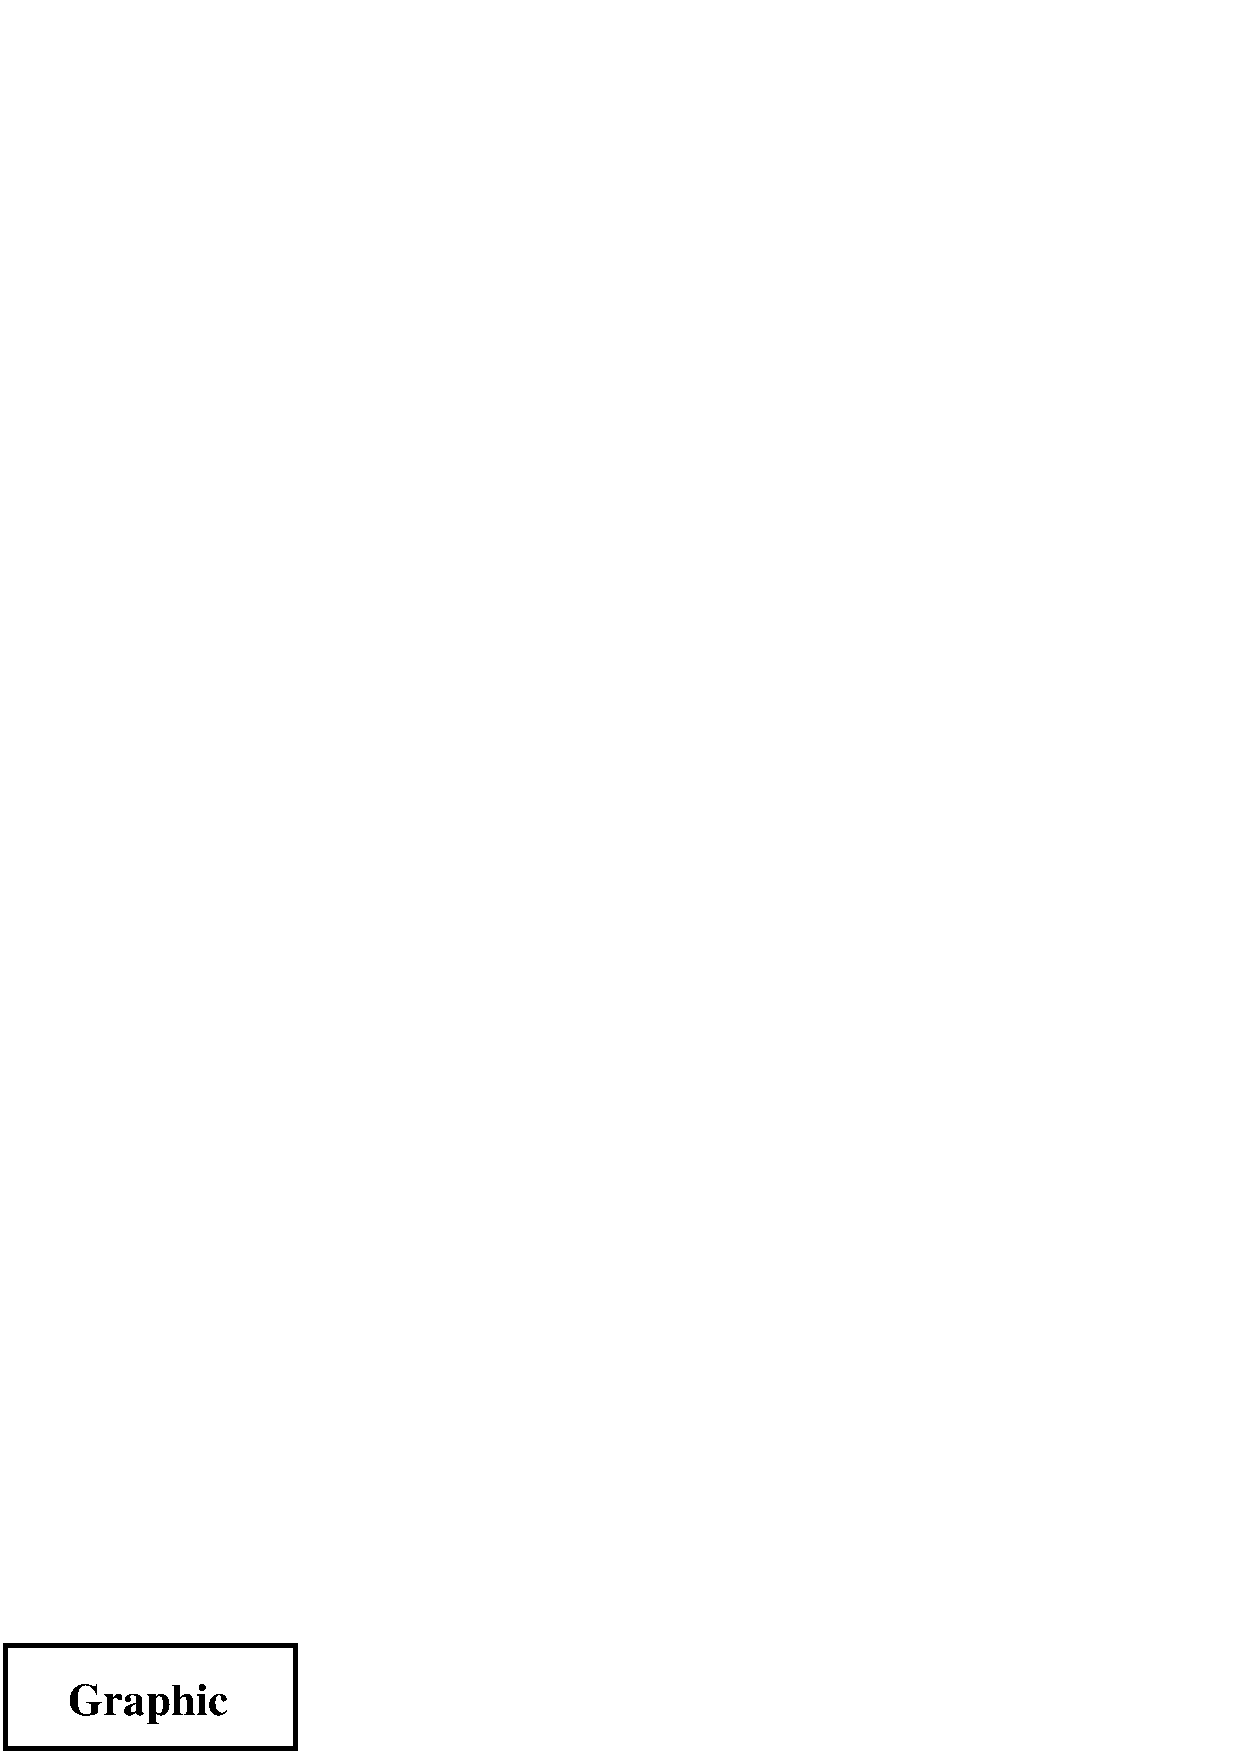
\includegraphics[width=3cm]{graphic}}
	\hspace{1cm}
	%%----start of second subfigure----
	\subcaptionbox{%
		Second Subfigure\label{fig:contfig:subtwo}}{%
		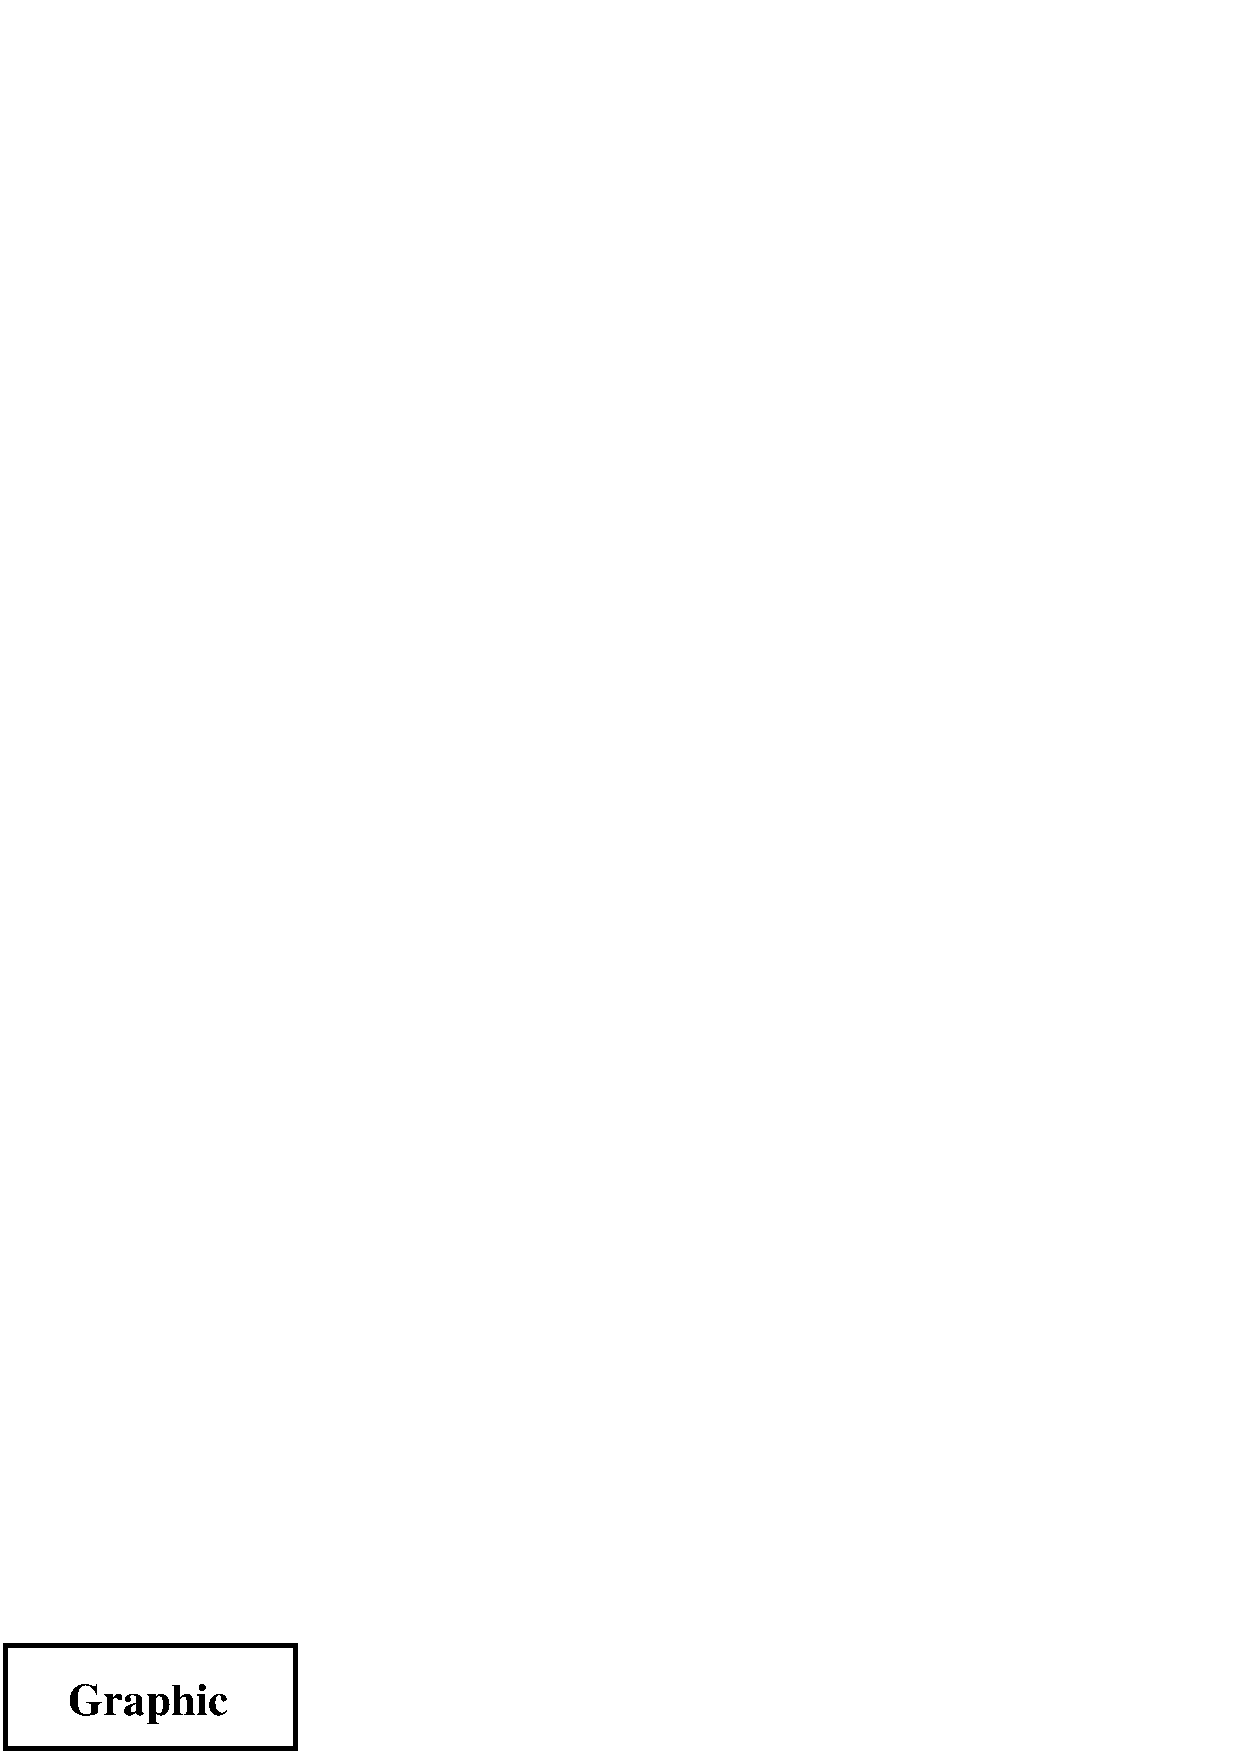
\includegraphics[width=3cm]{graphic}}
	\caption{Two Subfigures}
	\label{fig:contfig:one}
\end{figure}
\begin{figure}
	\ContinuedFloat
	\centering
	%%----start of third subfigure----
	\subcaptionbox{%
		Third Subfigure\label{fig:contfig:subthree}}{%
		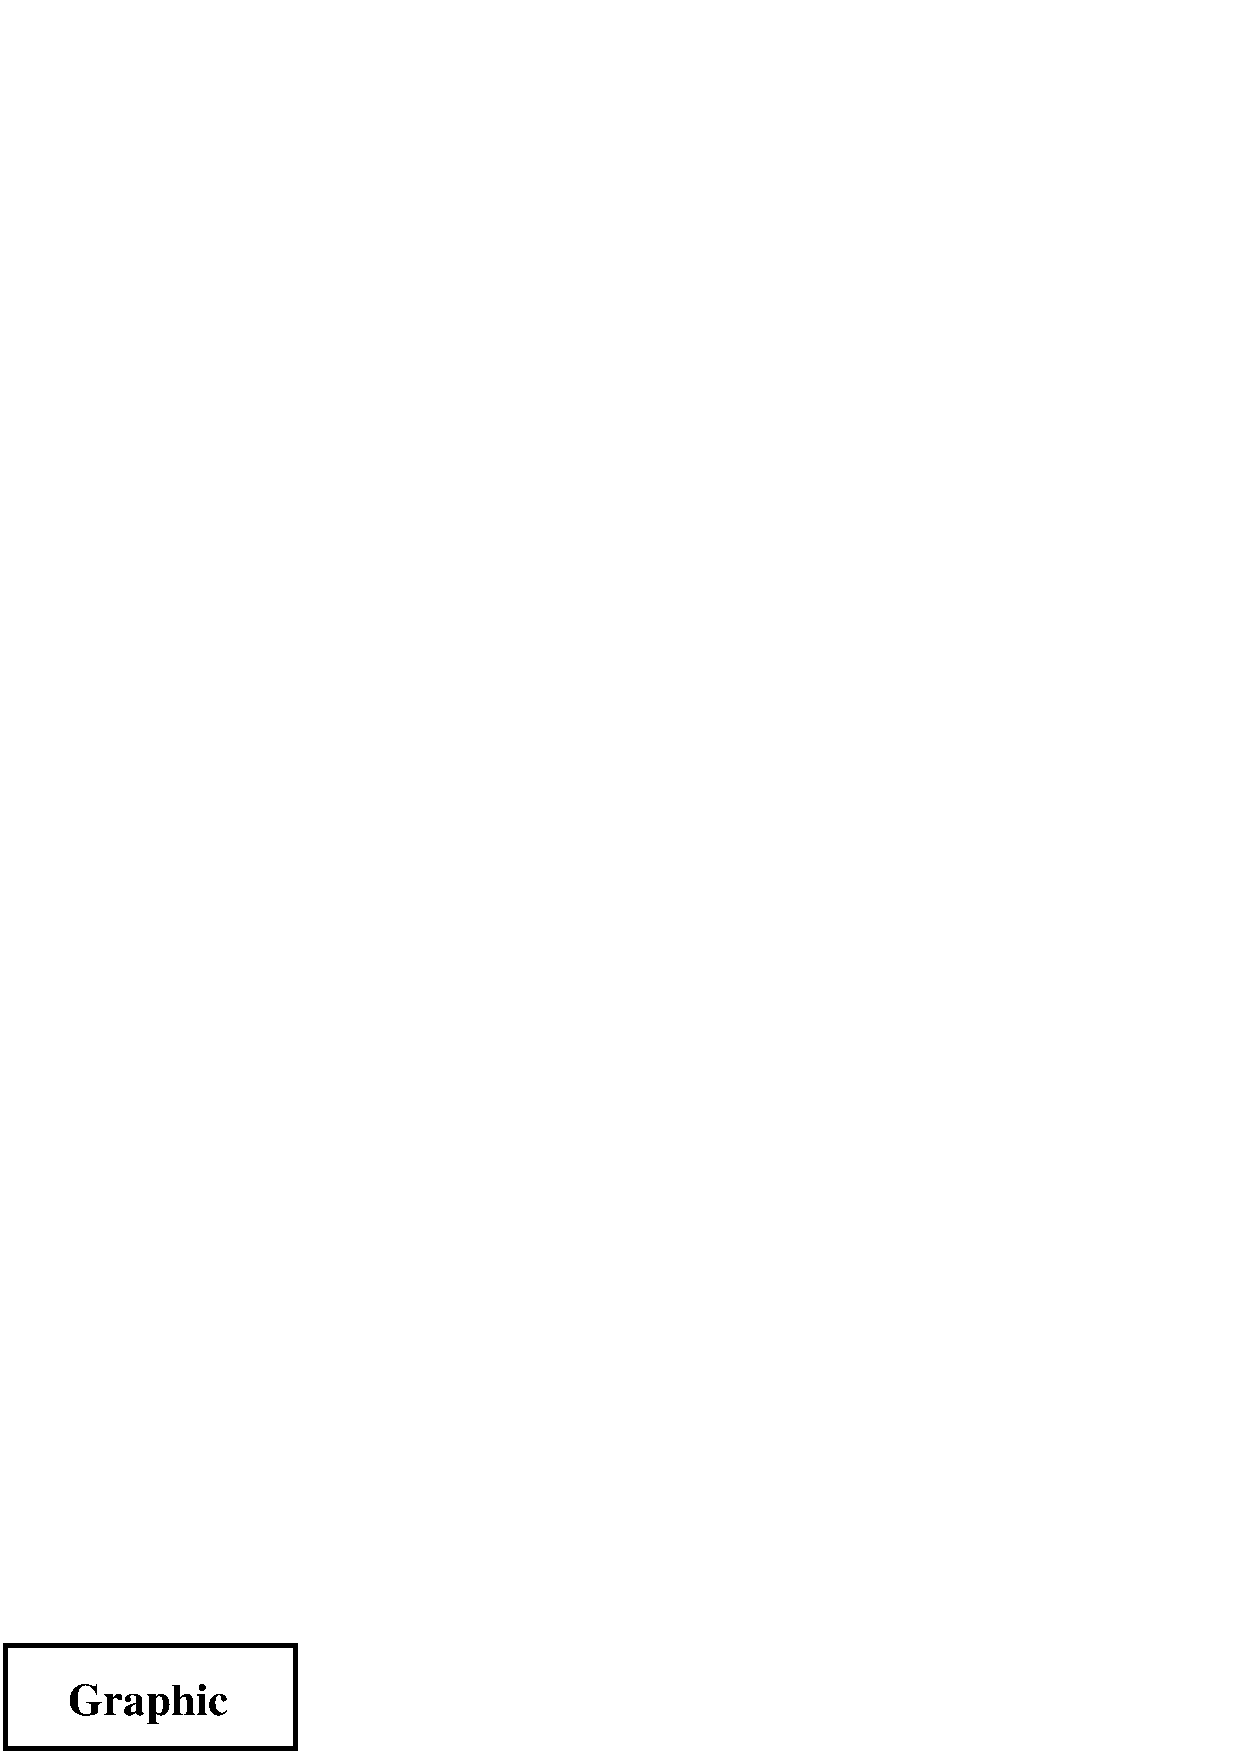
\includegraphics[width=3cm]{graphic}}
	\hspace{1cm}
	%%----start of fourth subfigure----
	\subcaptionbox{%
		Fourth Subfigure\label{fig:contfig:subfour}}{%
		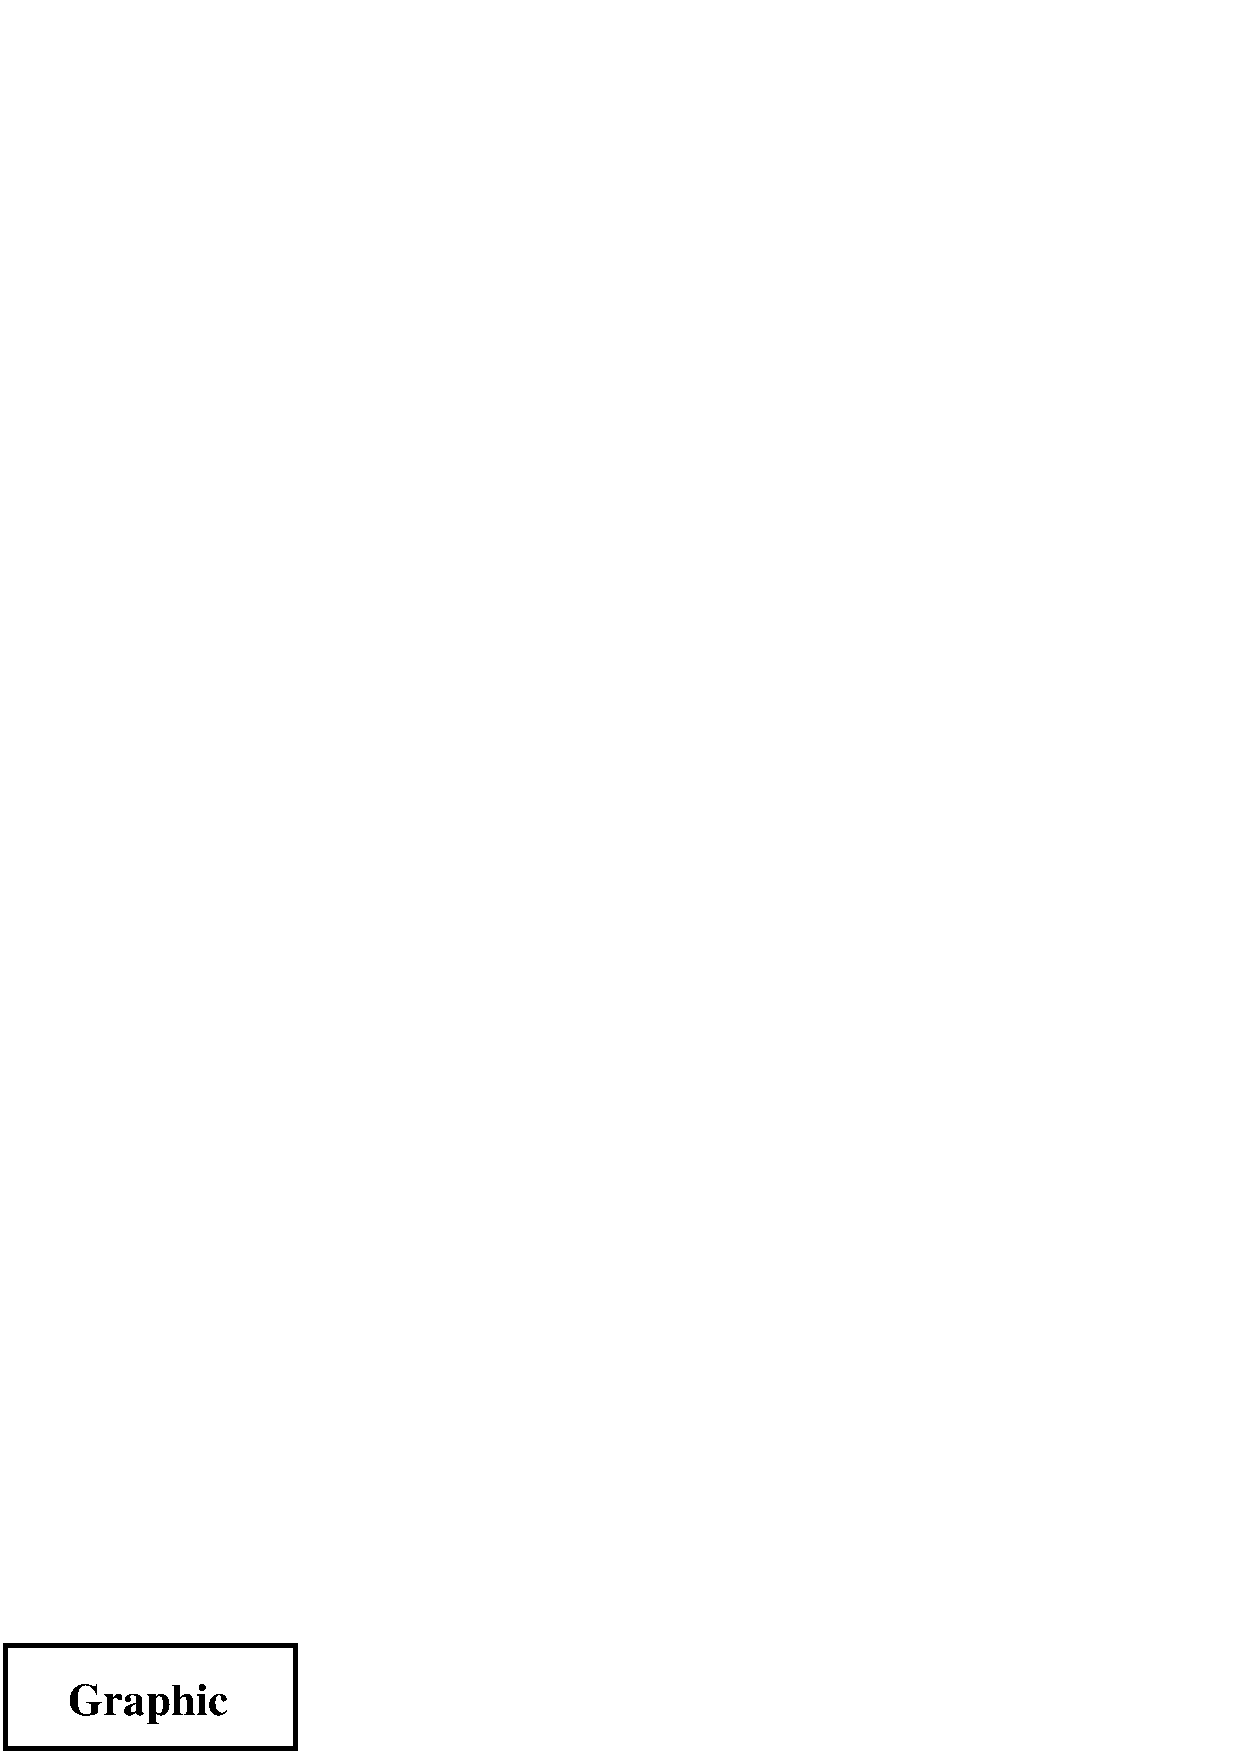
\includegraphics[width=3cm]{graphic}}
	\caption{Two Additional Subfigures}
	\label{fig:contfig:two}
\end{figure}
\end{lstlisting}
该代码片段会创建两个浮动体,
分别包含图~\ref{fig:contfig:subone}、\ref{fig:contfig:subtwo} 
以及图~\ref{fig:contfig:subthree}、\ref{fig:contfig:subfour}。
显然这四个子图可以放在同一个浮动体内,
但本例只是为了说明如何进行更大的子图分组。

注意 \cmd{ContinuedFloat} 命令不仅保持浮动体编号不变,而且确保第二个浮动体内的子图编号不会重置为 (a)。
此外两个浮动体的标题具有不同的引用标签(\texttt{fig:contfig:one} 和 \texttt{fig:contfig:two}),
但相应的 \cmd{ref} 引用值是相同的,
不过由于两个浮动体可能不同页,因此对应的 \cmd{pageref} 值可能不同。

\begin{figure}
	\centering
	%%----start of first subfigure----
	\subcaptionbox{%
		First Subfigure\label{fig:contfig:subone}}{%
		\resizebox{3cm}{!}{\usebox{\boxgraphic}}}
	\hspace{1cm}
	%%----start of second subfigure----
	\subcaptionbox{%
		Second Subfigure\label{fig:contfig:subtwo}}{%
		\resizebox{3cm}{!}{\usebox{\boxgraphic}}}
	\caption{Two Subfigures}
	\label{fig:contfig:one}
\end{figure}
\begin{figure}
	\ContinuedFloat
	\centering
	%%----start of third subfigure----
	\subcaptionbox{%
		Third Subfigure\label{fig:contfig:subthree}}{%
		\resizebox{\linewidth}{!}{\usebox{\boxgraphic}}}
	\hspace{1cm}
	%%----start of fourth subfigure----
	\subcaptionbox{%
		Fourth Subfigure\label{fig:contfig:subfour}}{%
		\resizebox{\linewidth}{!}{\usebox{\boxgraphic}}}
	\caption{Two Additional Subfigures}
	\label{fig:contfig:two}
\end{figure}

\section{图文混排}\label{sec:figintext}

在使用外部图形时,通常的是将其置于一个 \env{figure} 环境中,
由这一浮动环境来决定最后的位置是在页面的上方或下方。
但有的时候,许多使用者往往希望将图形放置在一个正文方格内,
或者置于页面的左右,也可能是在页面的的中间,四周包围者文本,
甚至放在文字的下方作为背景,或重叠放置。
这时,前面所介绍的只使用 \LaTeX{} 图形宏包套件就很难得到所希望的结果。
本节将介绍两个有用的图形宏包 \pkgi{wrapfig} 和 \pkgi{picinpar},
可以让你很容易地得到上述特殊效果。\footnote{
    图文混排这一部分来自于旧译本,并经过一些修改调整。
    旧译本还介绍了 \pkg{picins} 宏包,但该宏包用于 \LaTeX2.09,较新的发行版已无此宏包,故略去。——译注}


除了本节所介绍的宏包外,还有一些宏包也可完成同样的工作。
如 \pkgi{floatflt}\cite{floatflt-doc} 以及较新的\pkgi{cutwin}\cite{cutwin-doc} 也可用来将图形置于文本段落的一边。
而所介绍的宏包中,也有未涉及的内容,
进一步的研究可阅读这些宏包所附的帮助文件。

\subsection{Wrapfig 宏包}\label{ssec:wrapfig}

\pkg{Wrapfig} 宏包提供了 \envi{wrapfigure} 环境\footnote{
	\pkg{wrapfig} 也同时提供了 \envi{wraptable} 环境。}来排版窄小的图形,
使得该图形位于文本的一边,并使文本在其边上折行。

\env{wrapfigure}的用法为:
\begin{flushleft}
	\cmdMOMOM{begin}{wrapfigure}{\metacmd{行数}}{\metacmd{位置}}{\metacmd{外延长度}}{\metacmd{宽度}}\\
	\qquad\metacmd{图内容}\\
	\cmdM{end}{wrapfigure}
\end{flushleft}

这里\metacmd{行数}是指图形高度所占的文本行的数目。
如果不给出此选项,\pkg{wrapfig}会自动计算。
\metacmd{位置}是指图形相对于文本的位置,须给定下面四项的一个。
其中大写字母选项允许图形浮动,而小写字母选项则严格地将图形放在代码所在位置。
\begin{description}
	\item [\opt{r,R}] 表示图形位于文本的右边。
	\item [\opt{l,L}] 表示图形位于文本的左边。
	\item [\opt{i,I}] 表示图形位于页面靠里的一边(用在\opt{twoside}双面格式里)。
	\item [\opt{o,O}] 表示图形位于页面靠外的一边。
\end{description}
\metacmd{外延长度}是指图形超出文本边界的长度,缺省为 $0\pt$。
如果大于 $0\pt$,图形则会产生超出版心的效果。
\metacmd{宽度}则指图形的宽度。

\begin{wrapfigure}{r}{4.5cm}
	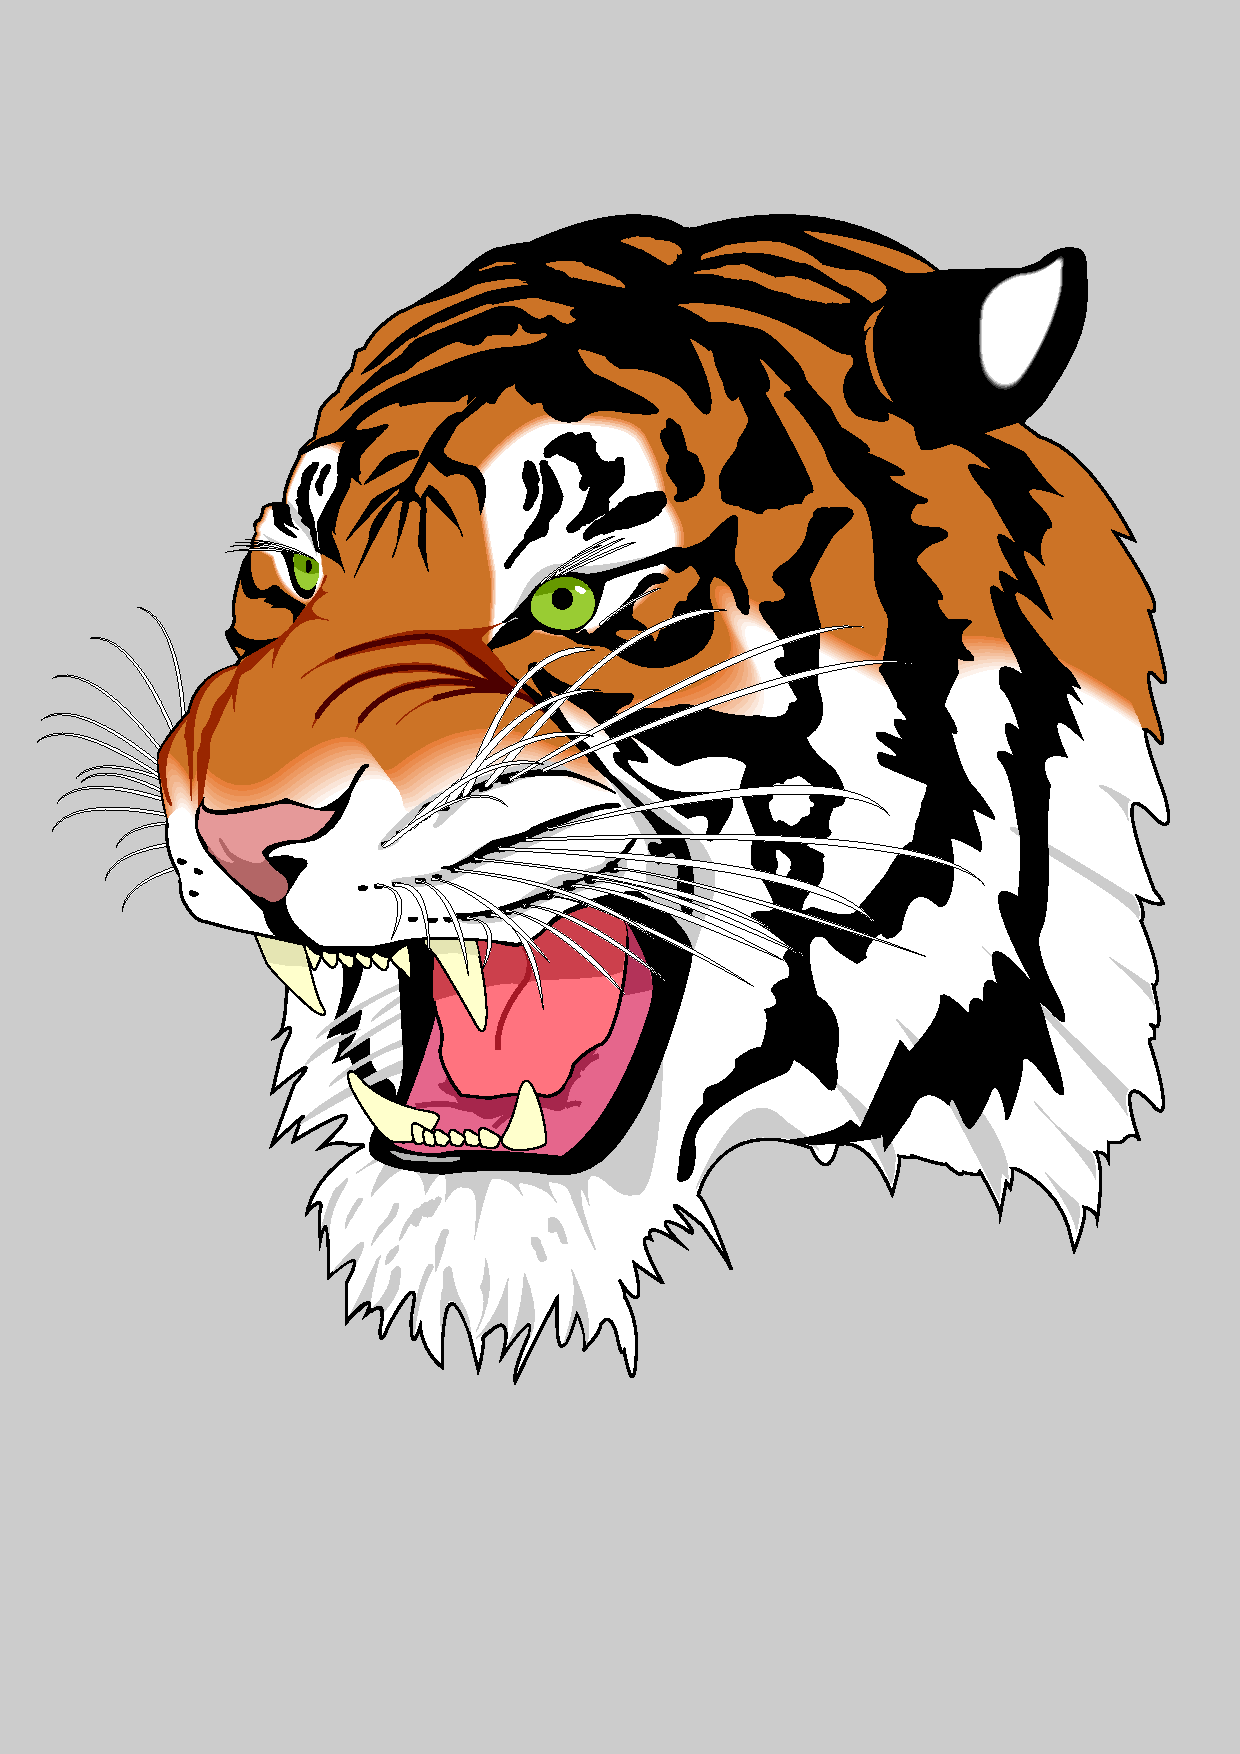
\includegraphics[width=4cm,clip]{tiger}
\end{wrapfigure}
在使用 \env{wrapfig} 环境进行图文绕排时需要注意下面几点:
\begin{itemize}
	\item 图文绕排通常需要多次手动定位。
	由于会受到修改其它排版格式的影响,因此应当在最后定稿前进行调整。
	\item \env{wrapfigure} 环境不能放置在跨页的地方。
	\item 从美学角度讲,图文混排只应当用于普通文本。
	章节标题、大块的公式与图形混排会很难看。
	图形放在列表的左边也很糟糕。(排版仍会允许,只是结果很差)
	如果是小型的公式则没有问题。
	\item 最好是在段落之间使用 \env{wrapfigure} 环境,
	如果想要在段落的内部使用,那么必须将 \env{wrapfigure} 环境放在可以自然断行的地方。
	\item 如果将 \env{wrapfigure} 放在 \cmd{parbox} 或小页环境等分组中,
	文本折行必须在这些分组前结束。
	\item 在折行的文本中,\cmd{linewidth} 并没有改变。
\end{itemize}

而浮动的绕排图形只会出现在以下之处:
\begin{itemize}
	\item 段落开始的地方;
	\item 当前页面有足够的空间,或者可以在下一页继续;
	\item 文本不是标题或列表;
	\item 文本没有环绕其它图形;
	\item 正文中的文本,而不是小页环境。
\end{itemize}

本节中的例子使用了如下命令:
\begin{lstlisting}
\begin{wrapfigure}{r}{4.5cm}
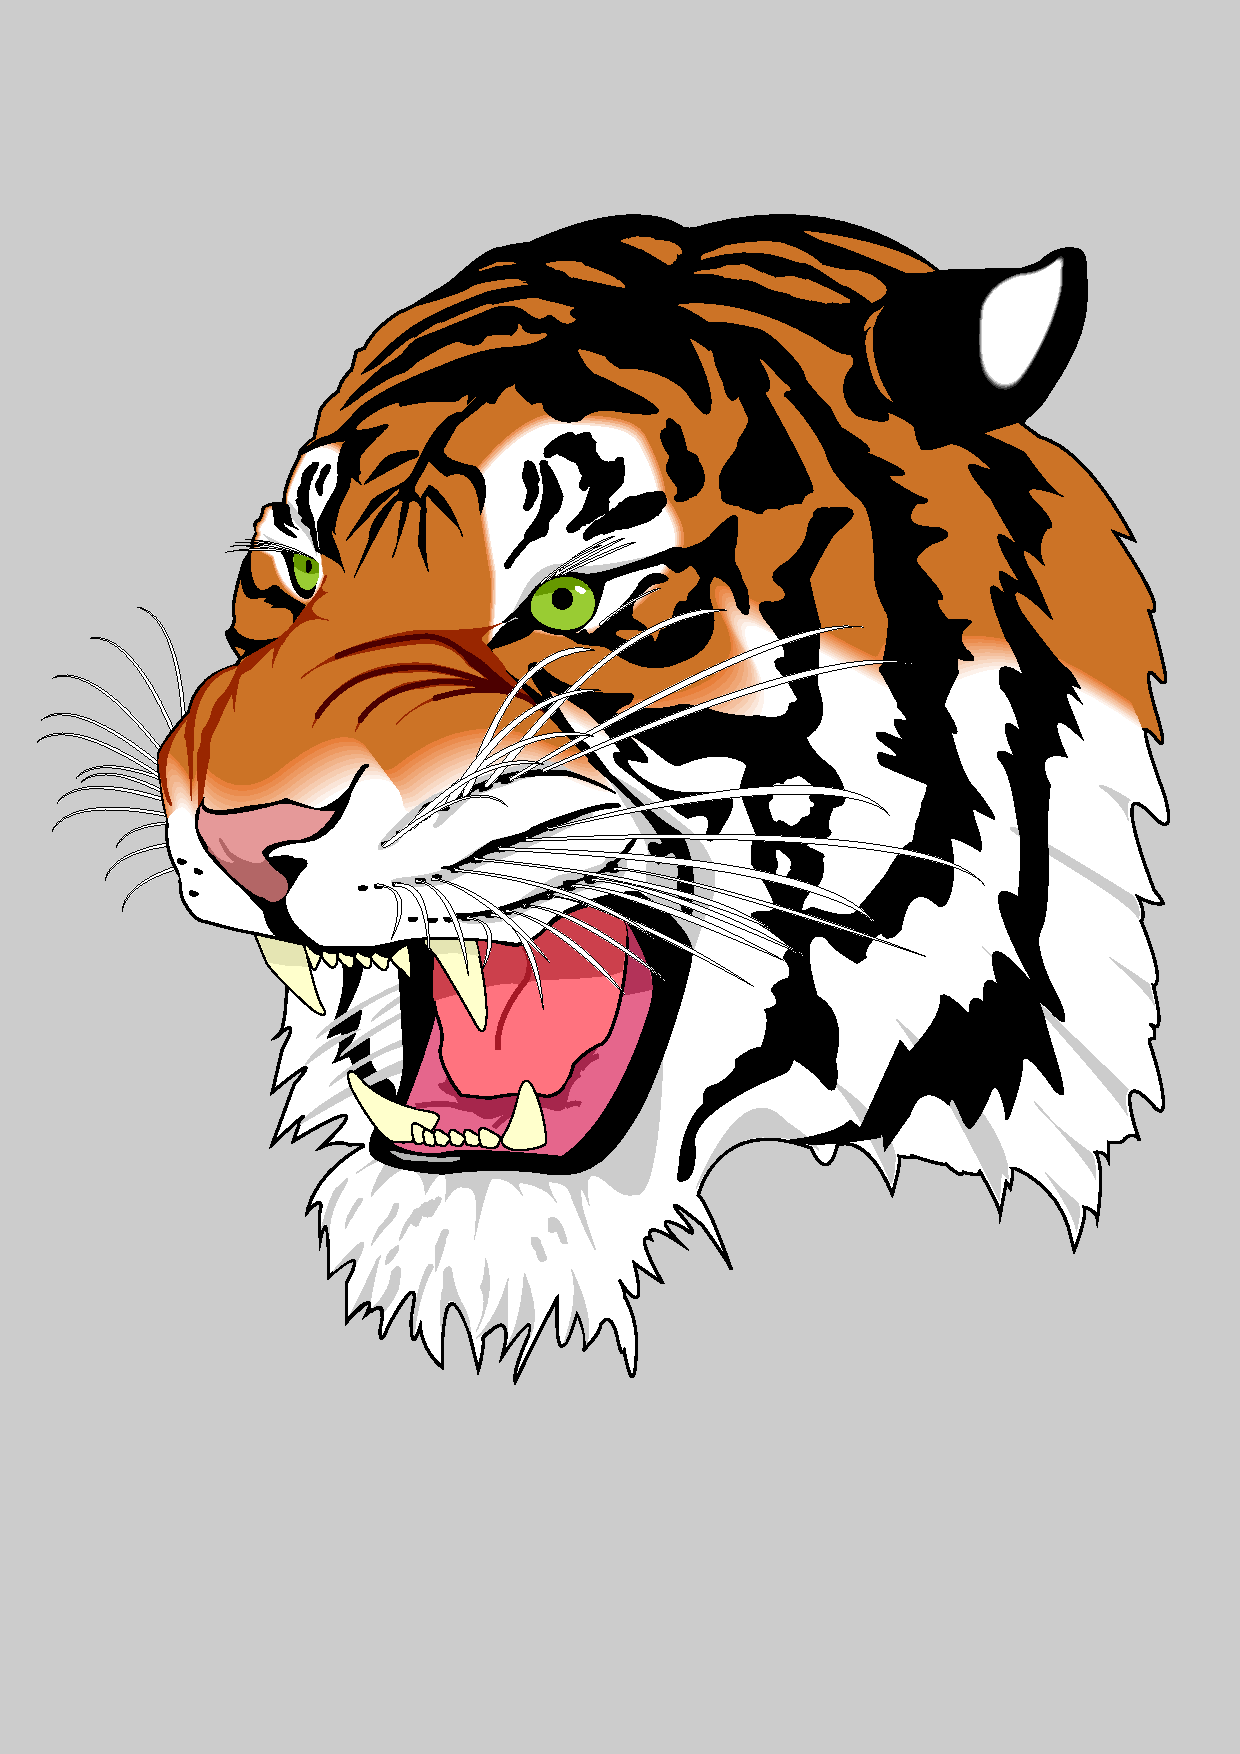
\includegraphics[width=4cm,clip]{tiger}
\end{wrapfigure}
在使用 \env{wrapfig} 环境进行图文绕排时需要注意下面几点:...
\end{lstlisting}


\subsection{Picinpar 宏包}\label{ssec:picinpar}

\pkgi{picinpar} 宏包定义了一个基本的环境 \envi{window},
以及两个变体环境 \envi{figwindow} 和 \envi{tabwindow}。
效果是在文本段落中打开一个“窗口”,在其中放入图形、文字和表格等。
这里我们主要讨论将图形放入文本段落的用法,其它的用法可参考 \pkg{picinpar} 的说明。

\begin{flushleft}
\cmdMO{begin}{window}{\metacmd{下降行数}, \metacmd{水平位置}, \metacmd{内容}, \metacmd{内容说明}}\\
\qquad\metacmd{绕排文字}\\
\cmdM{end}{window}
\end{flushleft}

\begin{flushleft}
	\cmdMO{begin}{figwindow}{\metacmd{下降行数}, \metacmd{水平位置}, \metacmd{图形}, \metacmd{图标题}}\\
	\qquad\metacmd{绕排文字}\\
	\cmdM{end}{figwindow}
\end{flushleft}

这里的\metacmd{下降行数}是指“窗口”开始前的行数。
\metacmd{水平位置}是指在段落中“窗口”的位置,缺省为 \opt{l},即居左。
另外两种是 \opt{c}(居中)和 \opt{r}(居右)。
第三个参数\metacmd{内容}是出现在“窗口”中的内容,
这在 \env{figwindow} 中就是要插入的图形。
第四个参数\metacmd{内容说明}则是对“窗口”内容的说明性文字,
这在 \env{figwindow} 中就是图形的标题。
下面是几个例子:

\CJKfamily{zhkai}
\begin{lstlisting}
\begin{window}[2,c,{\fcolorbox{morelight}{yellow}{%
	\shortstack{你在他乡 \\还 好 \\ 吗?}}},{}]
	可是哈卜拉姆再聪明...可是我偏不喜欢。」
\end{window}
\end{lstlisting}

\begin{window}[2,c,{\fcolorbox{morelight}{yellow}{%
		\shortstack{你在他乡 \\还好 \\ 吗?}}},{}]
	可是哈卜拉姆再聪明、再有学问,有一件事却是他不能解答的,因为包
    罗万象 的「可兰经」上也没有答案;如果你深深爱著的人,却深深的爱上了
	别人,有甚麽法子?白马带著她一步步的回到中原。白马已经老了,只能慢
	慢的走,但终是能回到中原的。江南有杨柳、桃花,有燕子、金鱼……汉人中
	有的是英俊勇武的少年,倜傥潇洒的少年……但这个美丽的姑娘就像古高昌国
	人那样固执:「那都是很好很好的,可是我偏不喜欢。」
\end{window}

\begin{lstlisting}
\begin{figwindow}[1,r,{\mbox{%
	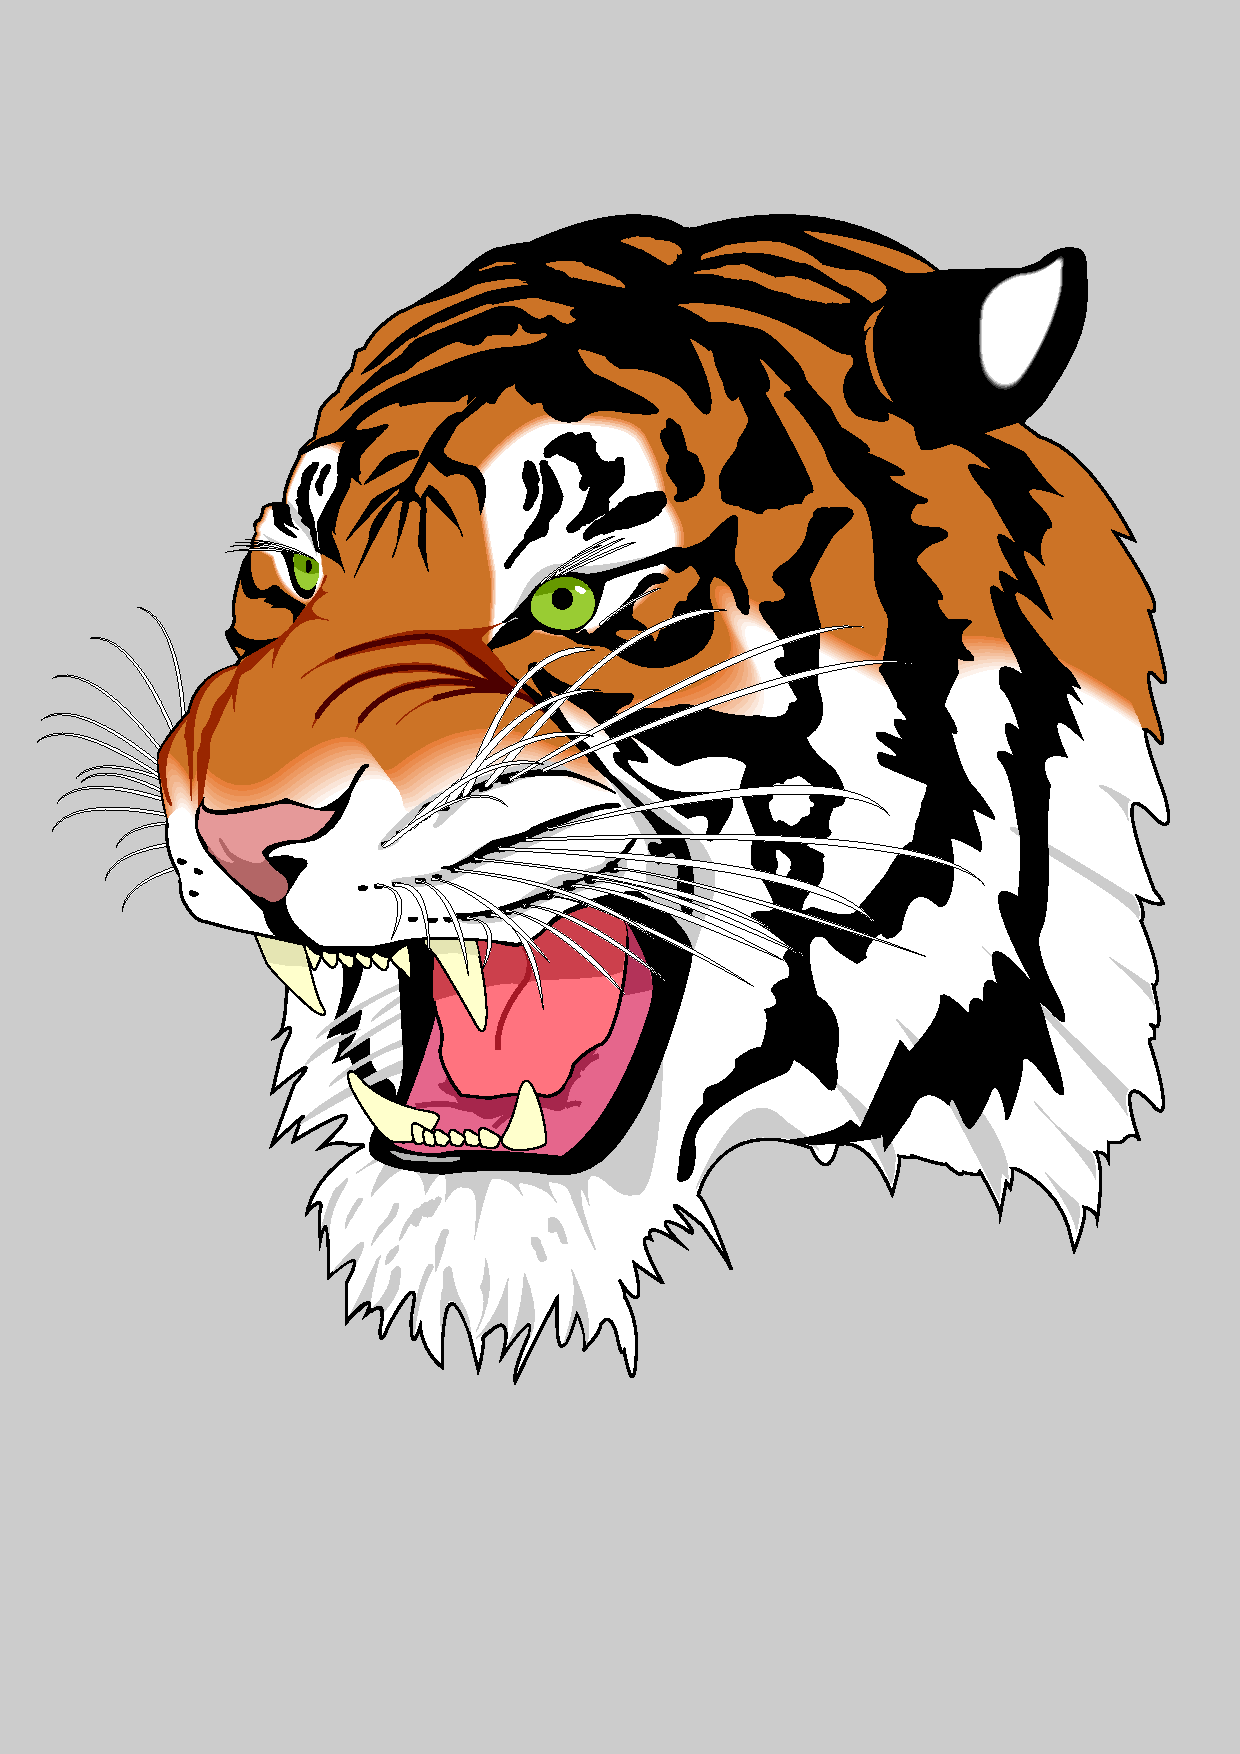
\includegraphics[width=2cm]{tiger}}},{Tiger}]
	可是哈卜拉姆再聪明...可是我偏不喜欢。」
\end{figwindow}
\end{lstlisting}

\begin{figwindow}[1,r,{\mbox{%
		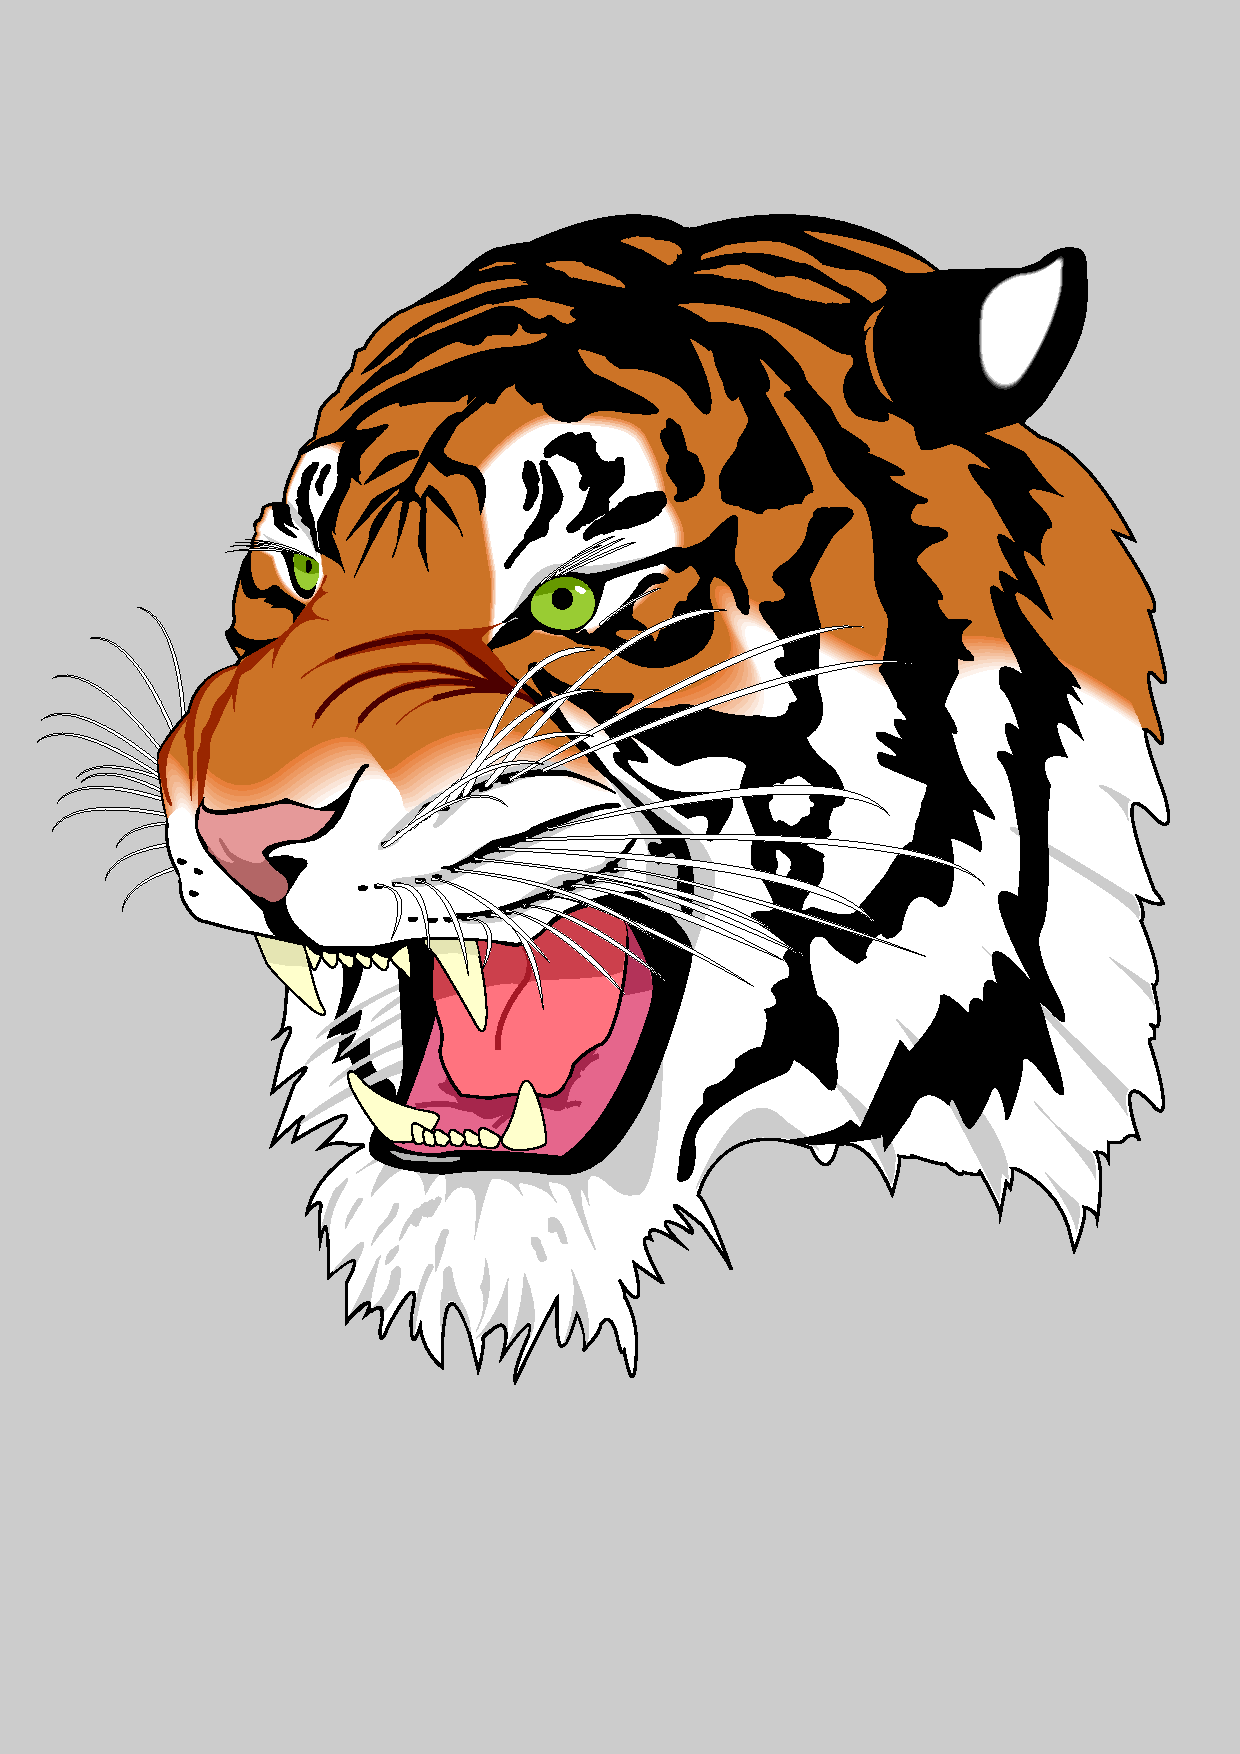
\includegraphics[width=2cm,clip]{tiger}}},{Tiger}]
	可是哈卜拉姆再聪明、再有学问,有一件事却是他不能解答的,因为包
	罗万象的「可兰经」上也没有答案;如果你深深爱著的人,却深深的爱上了
	别人,有甚麽法子?白马带著她一步步的回到中原。白马已经老了,只能慢
	慢的走,但终是能回到中原的。江南有杨柳、桃花,有燕子、金鱼……汉人中
	有的是英俊勇武的少年,倜傥潇洒的少年……但这个美丽的姑娘就像古高昌国
	人那样固执:「那都是很好很好的,可是我偏不喜欢。」
\end{figwindow}

\begin{lstlisting}
\begin{figwindow}[1,c,{\mbox{%
	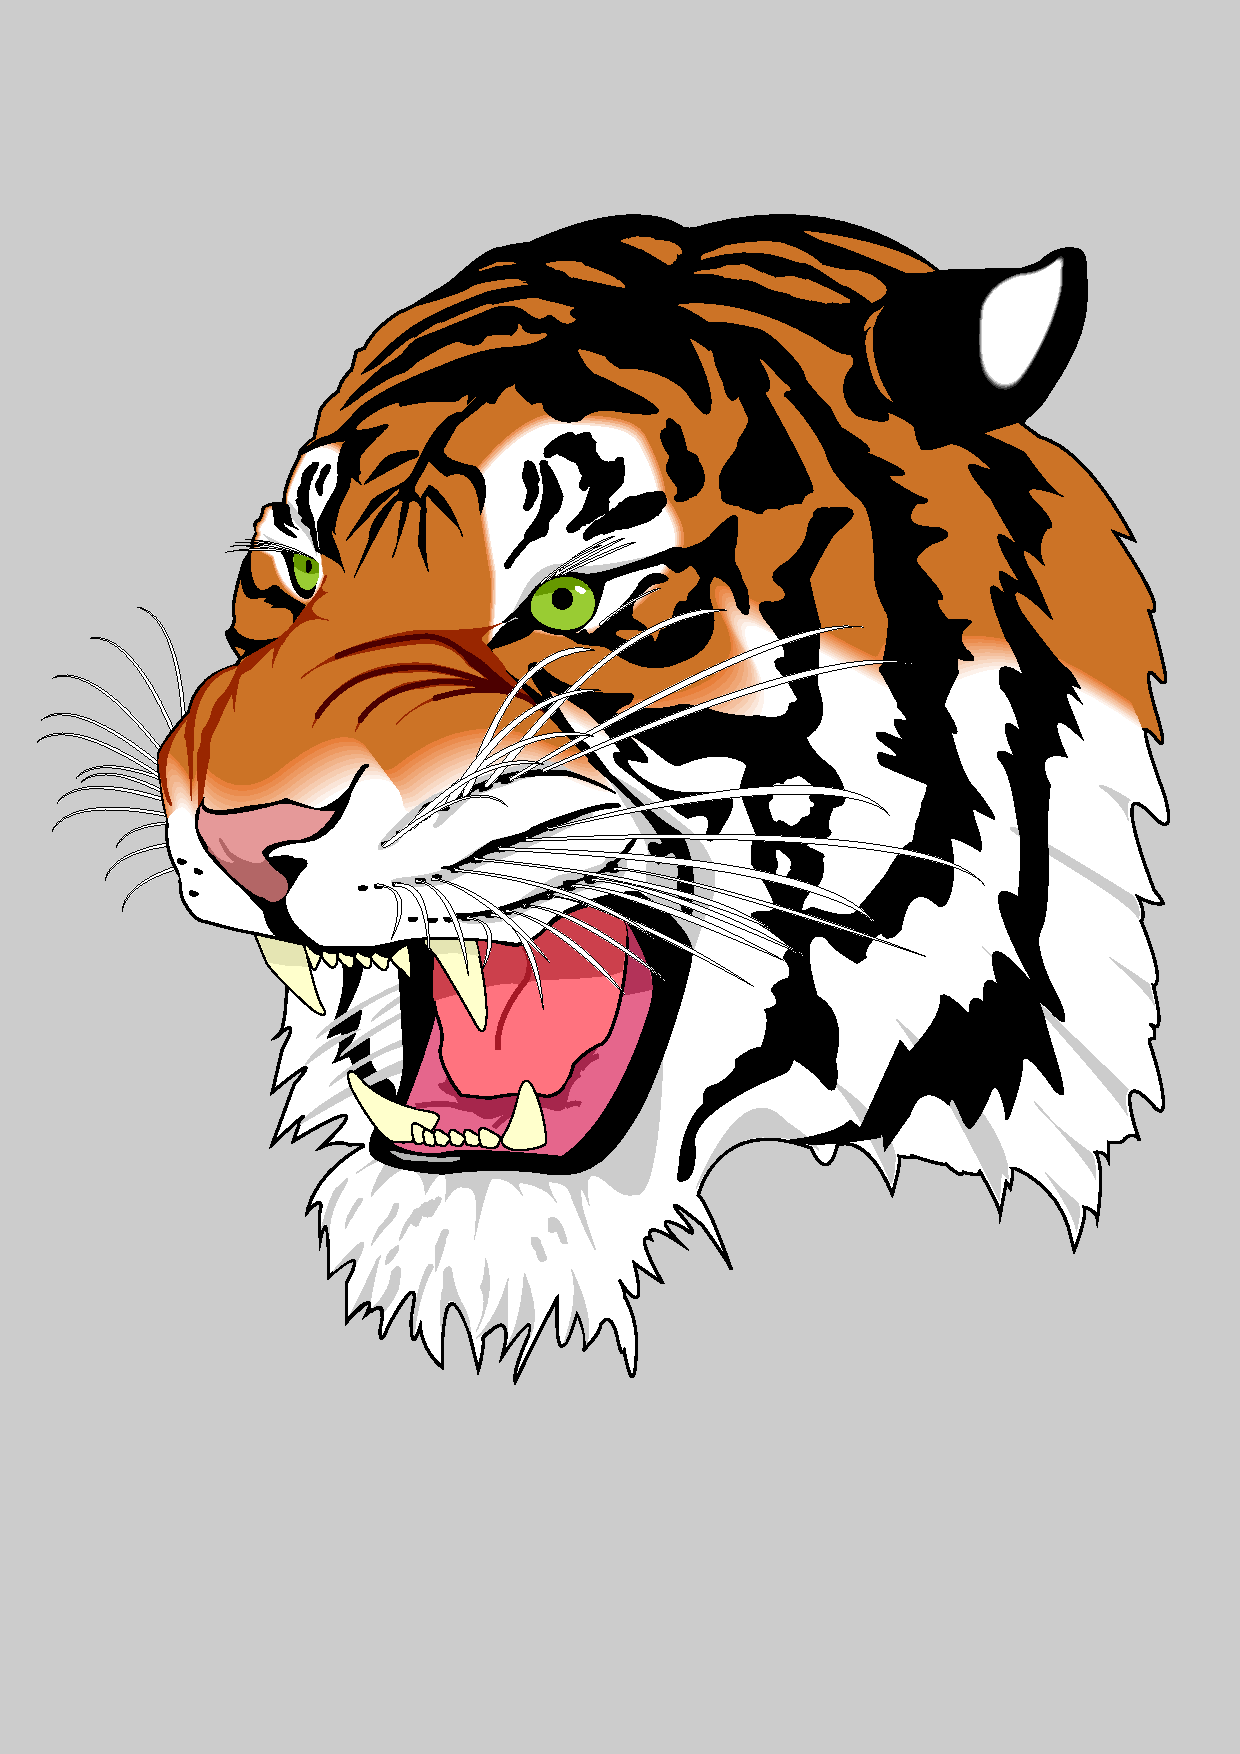
\includegraphics[width=2cm]{tiger}}},{Tiger}]
	可是哈卜拉姆再聪明...可是我偏不喜欢。」
\end{figwindow}
\end{lstlisting}

\begin{figwindow}[1,c,{\mbox{%
		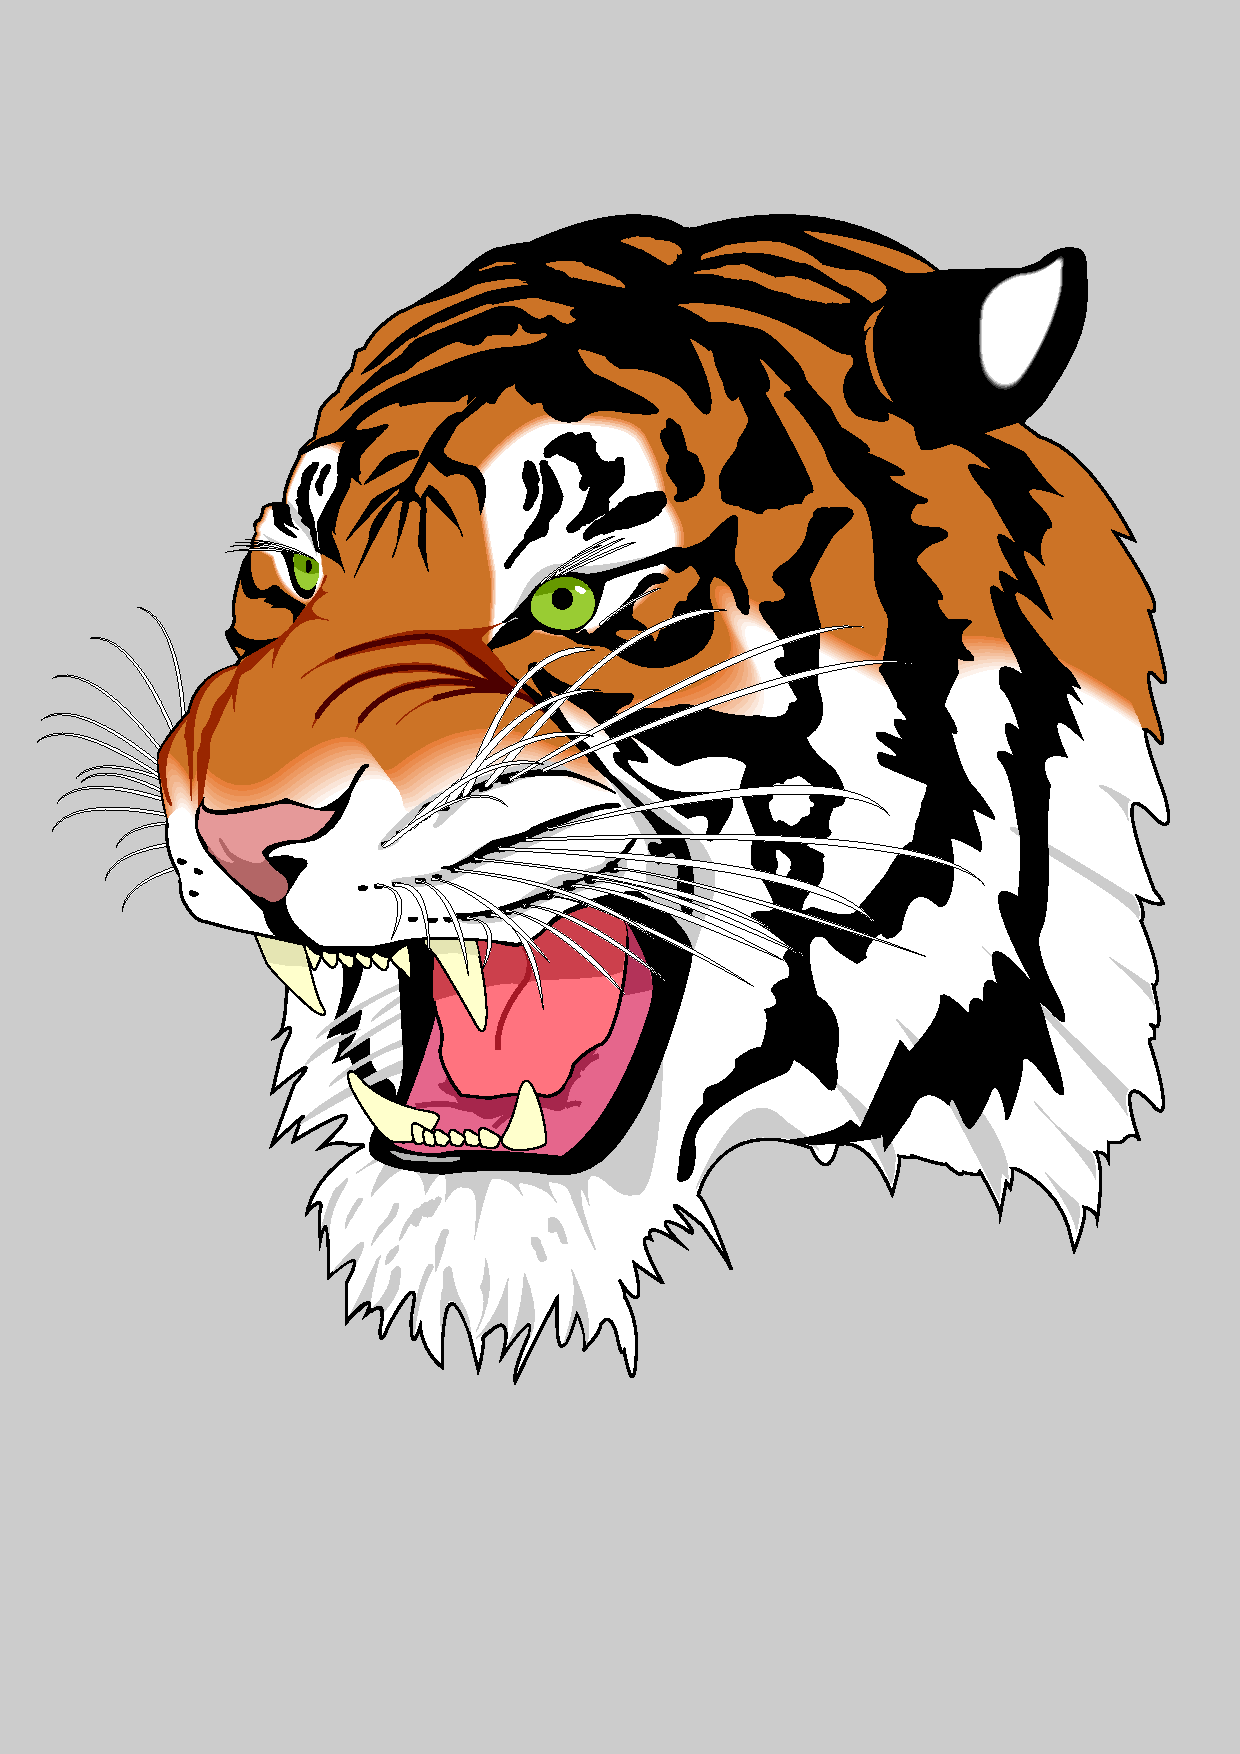
\includegraphics[width=2cm,clip]{tiger}}},{Tiger}]
	可是哈卜拉姆再聪明、再有学问,有一件事却是他不能解答的,因为包
	罗万象的「可兰经」上也没有答案;如果你深深爱著的人,却深深的爱上了
	别人,有甚麽法子?白马带著她一步步的回到中原。白马已经老了,只能慢
	慢的走,但终是能回到中原的。江南有杨柳、桃花,有燕子、金鱼……汉人中
	有的是英俊勇武的少年,倜傥潇洒的少年……但这个美丽的姑娘就像古高昌国
	人那样固执:「那都是很好很好的,可是我偏不喜欢。」
\end{figwindow}
\CJKfamily{zhsong}

在使用 \pkg{picinpar} 时要注意以下几点:
\begin{itemize}
	\item 不要在 \env{window} 环境中使用 \cmd{samepage}。
	\item 不要在 \env{window} 环境中使用 \cmd{footnote},
	代之用 \cmd{footnotemark} 标记角注,
	而将角注的内容在 \env{window} 环境外用 \cmd{footnotetext} 加入。
\end{itemize}

\endinput
